\PassOptionsToPackage{unicode=true}{hyperref} % options for packages loaded elsewhere
\PassOptionsToPackage{hyphens}{url}
%
\documentclass[10pt,xcolor=table,color={dvipsnames,usenames},ignorenonframetext,usepdftitle=false,french]{beamer}
\setbeamertemplate{caption}[numbered]
\setbeamertemplate{caption label separator}{: }
\setbeamercolor{caption name}{fg=normal text.fg}
\beamertemplatenavigationsymbolsempty
\usepackage{caption}
\captionsetup{skip=0pt,belowskip=0pt}
%\setlength\abovecaptionskip{-15pt}
\usepackage{lmodern}
\usepackage{amssymb,amsmath,mathtools,multirow}
\usepackage{float,hhline}
\usepackage{tikz}
\usepackage{mathtools}
\usepackage{ifxetex,ifluatex}
\usepackage{fixltx2e} % provides \textsubscript
\ifnum 0\ifxetex 1\fi\ifluatex 1\fi=0 % if pdftex
  \usepackage[T1]{fontenc}
  \usepackage[utf8]{inputenc}
  \usepackage{textcomp} % provides euro and other symbols
\else % if luatex or xelatex
  \usepackage{unicode-math}
  \defaultfontfeatures{Ligatures=TeX,Scale=MatchLowercase}
\fi
\usetheme[coding=utf8,language=english,
,titlepagelogo=img/SACElogo
]{TorinoTh}
% use upquote if available, for straight quotes in verbatim environments
\IfFileExists{upquote.sty}{\usepackage{upquote}}{}
% use microtype if available
\IfFileExists{microtype.sty}{%
\usepackage[]{microtype}
\UseMicrotypeSet[protrusion]{basicmath} % disable protrusion for tt fonts
}{}
\IfFileExists{parskip.sty}{%
\usepackage{parskip}
}{% else
\setlength{\parindent}{0pt}
\setlength{\parskip}{6pt plus 2pt minus 1pt}
}
\usepackage{hyperref}
\hypersetup{
            pdfauthor={Anna Smyk and Tanguy Barthelemy},
            pdfborder={0 0 0},
            breaklinks=true}
\urlstyle{same}  % don't use monospace font for urls
\newif\ifbibliography
\newlength{\cslhangindent}
\setlength{\cslhangindent}{1.5em}
\newlength{\csllabelwidth}
\setlength{\csllabelwidth}{3em}
\newenvironment{CSLReferences}[2] % #1 hanging-ident, #2 entry spacing
 {% don't indent paragraphs
  \setlength{\parindent}{0pt}
  % turn on hanging indent if param 1 is 1
  \ifodd #1 \everypar{\setlength{\hangindent}{\cslhangindent}}\ignorespaces\fi
  % set entry spacing
  \ifnum #2 > 0
  \setlength{\parskip}{#2\baselineskip}
  \fi
 }%
 {}
\usepackage{color}
\usepackage{fancyvrb}
\newcommand{\VerbBar}{|}
\newcommand{\VERB}{\Verb[commandchars=\\\{\}]}
\DefineVerbatimEnvironment{Highlighting}{Verbatim}{commandchars=\\\{\}}
% Add ',fontsize=\small' for more characters per line
\usepackage{framed}
\definecolor{shadecolor}{RGB}{248,248,248}
\newenvironment{Shaded}{\begin{snugshade}}{\end{snugshade}}
\newcommand{\AlertTok}[1]{\textcolor[rgb]{0.94,0.16,0.16}{#1}}
\newcommand{\AnnotationTok}[1]{\textcolor[rgb]{0.56,0.35,0.01}{\textbf{\textit{#1}}}}
\newcommand{\AttributeTok}[1]{\textcolor[rgb]{0.77,0.63,0.00}{#1}}
\newcommand{\BaseNTok}[1]{\textcolor[rgb]{0.00,0.00,0.81}{#1}}
\newcommand{\BuiltInTok}[1]{#1}
\newcommand{\CharTok}[1]{\textcolor[rgb]{0.31,0.60,0.02}{#1}}
\newcommand{\CommentTok}[1]{\textcolor[rgb]{0.56,0.35,0.01}{\textit{#1}}}
\newcommand{\CommentVarTok}[1]{\textcolor[rgb]{0.56,0.35,0.01}{\textbf{\textit{#1}}}}
\newcommand{\ConstantTok}[1]{\textcolor[rgb]{0.00,0.00,0.00}{#1}}
\newcommand{\ControlFlowTok}[1]{\textcolor[rgb]{0.13,0.29,0.53}{\textbf{#1}}}
\newcommand{\DataTypeTok}[1]{\textcolor[rgb]{0.13,0.29,0.53}{#1}}
\newcommand{\DecValTok}[1]{\textcolor[rgb]{0.00,0.00,0.81}{#1}}
\newcommand{\DocumentationTok}[1]{\textcolor[rgb]{0.56,0.35,0.01}{\textbf{\textit{#1}}}}
\newcommand{\ErrorTok}[1]{\textcolor[rgb]{0.64,0.00,0.00}{\textbf{#1}}}
\newcommand{\ExtensionTok}[1]{#1}
\newcommand{\FloatTok}[1]{\textcolor[rgb]{0.00,0.00,0.81}{#1}}
\newcommand{\FunctionTok}[1]{\textcolor[rgb]{0.00,0.00,0.00}{#1}}
\newcommand{\ImportTok}[1]{#1}
\newcommand{\InformationTok}[1]{\textcolor[rgb]{0.56,0.35,0.01}{\textbf{\textit{#1}}}}
\newcommand{\KeywordTok}[1]{\textcolor[rgb]{0.13,0.29,0.53}{\textbf{#1}}}
\newcommand{\NormalTok}[1]{#1}
\newcommand{\OperatorTok}[1]{\textcolor[rgb]{0.81,0.36,0.00}{\textbf{#1}}}
\newcommand{\OtherTok}[1]{\textcolor[rgb]{0.56,0.35,0.01}{#1}}
\newcommand{\PreprocessorTok}[1]{\textcolor[rgb]{0.56,0.35,0.01}{\textit{#1}}}
\newcommand{\RegionMarkerTok}[1]{#1}
\newcommand{\SpecialCharTok}[1]{\textcolor[rgb]{0.00,0.00,0.00}{#1}}
\newcommand{\SpecialStringTok}[1]{\textcolor[rgb]{0.31,0.60,0.02}{#1}}
\newcommand{\StringTok}[1]{\textcolor[rgb]{0.31,0.60,0.02}{#1}}
\newcommand{\VariableTok}[1]{\textcolor[rgb]{0.00,0.00,0.00}{#1}}
\newcommand{\VerbatimStringTok}[1]{\textcolor[rgb]{0.31,0.60,0.02}{#1}}
\newcommand{\WarningTok}[1]{\textcolor[rgb]{0.56,0.35,0.01}{\textbf{\textit{#1}}}}
% Prevent slide breaks in the middle of a paragraph:
\widowpenalties 1 10000
\raggedbottom
\AtBeginPart{
  \let\insertpartnumber\relax
  \let\partname\relax
  \frame{\partpage}
}
\AtBeginSection{
  \ifbibliography
  \else
    \begin{frame}[noframenumbering]{Contents}
    \tableofcontents[currentsection, hideothersubsections]
    \end{frame}
  \fi
}
\setlength{\emergencystretch}{3em}  % prevent overfull lines
\providecommand{\tightlist}{%
  %\setlength{\itemsep}{0pt}
  \setlength{\parskip}{0pt}
  }
\setcounter{secnumdepth}{0}

% set default figure placement to htbp
\makeatletter
\def\fps@figure{htbp}
\makeatother

\usepackage{dsfont}
\usepackage{stmaryrd}
\usepackage[normalem]{ulem}
\usepackage{fontawesome5}
\usepackage{tikz,pgfplots}
\pgfplotsset{compat=1.17}
\pgfplotsset{samples=100}
\usepackage{animate}
 \usepackage{booktabs}

\usepackage{colortbl}

\DeclareMathOperator{\Cov}{Cov}
\newcommand{\cov}[2]{\Cov\left( #1\,,\,#2 \right)}

\DeclareMathOperator{\e}{e}
\renewcommand{\P}{\mathds{P}} %Apparement \P existe déjà ?
\newcommand\N{\mathds{N}}
\newcommand\R{\mathds{R}}


\newcommand\1{\mathds{1}}
\newcommand{\E}[2][]{{\mathds{E}}_{#1}
  \def\temp{#2}\ifx\temp\empty
  \else
    \left[#2\right]
  \fi
}
\newcommand{\V}[2][]{{\mathds{V}}_{#1}
  \def\temp{#2}\ifx\temp\empty
  \else
    \left[#2\right]
  \fi
}
\newcommand\ud{\,\mathrm{d}}


% blocks
\usepackage{environ}
\usepackage[tikz]{bclogo}

\tikzstyle{titlestyle} =[draw=black!80,fill=black!20, text=black,
 right=10pt, rounded corners]
\mdfdefinestyle{symmaryboxstyle}{
	linecolor=black!80, backgroundcolor = black!5,
	skipabove=\baselineskip, innertopmargin=\baselineskip,
	innerbottommargin=\baselineskip,
	userdefinedwidth=\textwidth,
	middlelinewidth=1.2pt, roundcorner=5pt,
	skipabove={\dimexpr0.5\baselineskip+\topskip\relax},
	frametitleaboveskip=\dimexpr-\ht\strutbox\relax,
	innerlinewidth=0pt,
}
\NewEnviron{summary}{%
\begin{mdframed}[style=symmaryboxstyle]
\vspace{-0.5em}
\BODY
\end{mdframed}
}
\makeatletter
% Open `\noalign` and check for overlay specification:
\def\rowcolor{\noalign{\ifnum0=`}\fi\bmr@rowcolor}
\newcommand<>{\bmr@rowcolor}{%
    \alt#1%
        {\global\let\CT@do@color\CT@@do@color\@ifnextchar[\CT@rowa\CT@rowb}% Rest of original `\rowcolor`
        {\ifnum0=`{\fi}\@gooble@rowcolor}% End `\noalign` and gobble all arguments of `\rowcolor`.
}
% Gobble all normal arguments of `\rowcolor`:
\newcommand{\@gooble@rowcolor}[2][]{\@gooble@rowcolor@}
\newcommand{\@gooble@rowcolor@}[1][]{\@gooble@rowcolor@@}
\newcommand{\@gooble@rowcolor@@}[1][]{\ignorespaces}

\newcommand{\rowc}[1]{\only<#1>{\\\rowcolor{processblue!40}}}
%\newcommand{\rowc}[1]{{\rowcolor<#1>{processblue!30}}
\newcommand{\cellc}[1]{\only<#1>{\cellcolor{processblue!40}}}
\newcommand{\supsp}[1]{\visible<#1>{\\}}

\title{Using JDemetra+ in R: from version 2 to version 3\\
Presentation 2: Seasonal adjustment in R}
\ateneo{TSACE Webinar, Wednesday December 14th 2022}
\author{Anna Smyk and Tanguy Barthelemy}
\date{}


\setrellabel{}

\setcandidatelabel{}

\rel{}
\division{With the collaboration of Alain Quartier-la-tente\\}

\departement{}
\makeatletter
\let\@@magyar@captionfix\relax
\makeatother


\begin{document}
\begin{frame}[plain,noframenumbering]
\titlepage
\end{frame}

\hypertarget{introduction}{%
\section{Introduction}\label{introduction}}

\begin{frame}{Outline table}
\protect\hypertarget{outline-table}{}
\end{frame}

\begin{frame}{Data formats}
\protect\hypertarget{data-formats}{}
here, no workspace structure - assets - shortcomings
\end{frame}

\begin{frame}{SA process}
\protect\hypertarget{sa-process}{}
\begin{itemize}
\tightlist
\item
  testing for seasonality
\item
  pre treatement
\item
  create customisezd variables for pretratement
\item
  decomposition
\item
  output series
\item
  diagnostics
\item
  customize parameters
\item
  repeat..
\end{itemize}
\end{frame}

\begin{frame}{rjd3 suite of packages for SA}
\protect\hypertarget{rjd3-suite-of-packages-for-sa}{}
in v2 :

in v3: more tools (tests,\ldots)
\end{frame}

\hypertarget{x13-and-some-tramo-seats}{%
\section{X13 (\ldots and some
Tramo-seats)}\label{x13-and-some-tramo-seats}}

\hypertarget{quick-launch-with-default-specifications}{%
\subsection{Quick Launch with default
specifications}\label{quick-launch-with-default-specifications}}

\begin{frame}[fragile]{Quick Launch with default specifications (1)}
\protect\hypertarget{quick-launch-with-default-specifications-1}{}
specifications - x13 - regarima - x11 (one less spec in default x13)

\begin{itemize}
\tightlist
\item
  Specification: created with \texttt{spec\_x11\_default()},
  \texttt{spec\_x13\_default()}, \texttt{spec\_regarima\_default()}
\end{itemize}

spec\_regarima\_default(name = c(``rg4'', ``rg0'', ``rg1'', ``rg2c'',
``rg3'', ``rg5c''))

spec\_x13\_default(name = c(``rsa4'', ``rsa0'', ``rsa1'', ``rsa2c'',
``rsa3'', ``rsa5c''))

spec\_x11\_default()
\end{frame}

\begin{frame}[fragile]{Quick Launch with default specifications (2)}
\protect\hypertarget{quick-launch-with-default-specifications-2}{}
\begin{itemize}
\tightlist
\item
  Apply model with \texttt{x11()}, \texttt{x13()}, \texttt{fast.x13()},
  \texttt{regarima()}, \texttt{fast.regarima()}
\end{itemize}
\end{frame}

\begin{frame}[fragile,allowframebreaks]{Running SA estimation process}
\protect\hypertarget{running-sa-estimation-process}{}
In version 2 \footnotesize

\begin{Shaded}
\begin{Highlighting}[]
\CommentTok{\# X13}
\NormalTok{sa\_x13\_v2}\OtherTok{\textless{}{-}}\NormalTok{RJDemetra}\SpecialCharTok{::}\FunctionTok{x13}\NormalTok{(y\_raw, }\AttributeTok{spec =}\StringTok{"RSA5c"}\NormalTok{)}

\CommentTok{\#Tramo{-}Seats}
\NormalTok{sa\_ts\_v2}\OtherTok{\textless{}{-}}\NormalTok{RJDemetra}\SpecialCharTok{::}\FunctionTok{tramoseats}\NormalTok{(y\_raw, }\AttributeTok{spec =}\StringTok{"RSAfull"}\NormalTok{)}
\end{Highlighting}
\end{Shaded}

In version 3 \footnotesize

\begin{Shaded}
\begin{Highlighting}[]
\CommentTok{\#X13}
\NormalTok{sa\_x13\_v3 }\OtherTok{\textless{}{-}}\NormalTok{ rjd3x13}\SpecialCharTok{::}\FunctionTok{x13}\NormalTok{(y\_raw, }\AttributeTok{spec=} \StringTok{"RSA5"}\NormalTok{)}
\NormalTok{sa\_x13\_v3}
\end{Highlighting}
\end{Shaded}

\begin{verbatim}
## RegARIMA
## Log-transformation: yes 
## SARIMA model:  (0,1,1) (0,1,1) 
## 
## Coefficients
##           Estimate Std. Error T-stat
## theta(1)  -0.72466    0.03740 -19.38
## btheta(1) -0.56372    0.04992 -11.29
## 
## Regression model:
##            Estimate Std. Error T-stat
## monday     0.016430   0.008647  1.900
## tuesday    0.012493   0.008603  1.452
## wednesday  0.006496   0.008621  0.754
## thursday  -0.003046   0.008598 -0.354
## friday     0.019581   0.008638  2.267
## saturday  -0.020445   0.008608 -2.375
## easter    -0.045446   0.017158 -2.649
## Number of observations:  354 
## Number of effective observations:  341 
## Number of parameters:  10 
## 
## Loglikelihood:  374.7681 
## Adjusted loglikelihood:  -1077.716 
## 
## Standard error of the regression (ML estimate):  0.07999264 
## AIC:  2175.432 
## AICC:  2176.099 
## BIC:  2213.751 
## 
## 
## Decomposition
## Monitoring and Quality Assessment Statistics: 
##     M stats
## m1    0.986
## m2    0.660
## m3    1.888
## m4    0.262
## m5    1.877
## m6    0.140
## m7    0.374
## m8    0.823
## m9    0.441
## m10   0.557
## m11   0.484
## q     0.799
## qm2   0.816
## 
## Final filters: 
## Seasonal filter:  
## Trend filter: 23 terms Henderson moving average
## 
## Diagnostics
## Relative contribution of the components to the stationary
## portion of the variance in the original series,
## after the removal of the long term trend (in %)
## 
##            Component
##  cycle        35.745
##  seasonal     49.917
##  irregular     6.601
##  calendar      2.726
##  others        0.000
##  total        94.989
## 
## Residual seasonality tests
##                 P.value
##  seas.ftest.i     0.977
##  seas.ftest.sa    0.992
##  seas.qstest.i    1.000
##  seas.qstest.sa   1.000
##  td.ftest.i       0.999
##  td.ftest.sa      0.999
## 
## 
## Final
## Last values
##             series       sa    trend seas       irr
## Jul 2018 108.12963 125.7729 112.5273    1 1.1177102
## Aug 2018  90.03625 116.6883 113.3824    1 1.0291574
## Sep 2018 116.46355 112.2071 113.8818    1 0.9852950
## Oct 2018 124.07923 109.5869 113.9926    1 0.9613510
## Nov 2018 136.04300 119.6826 113.7513    1 1.0521420
## Dec 2018 113.17850 124.2718 113.2503    1 1.0973202
## Jan 2019 108.28574 108.9028 112.6145    1 0.9670404
## Feb 2019 110.21151 114.3220 111.9838    1 1.0208800
## Mar 2019 122.43580 111.6401 111.4757    1 1.0014743
## Apr 2019 108.64593 108.2331 111.1456    1 0.9737949
## May 2019 111.25296 111.2931 110.9967    1 1.0026702
## Jun 2019 109.35264 105.3926 111.0227    1 0.9492889
\end{verbatim}

\begin{Shaded}
\begin{Highlighting}[]
\CommentTok{\#Tramo seats}
\NormalTok{sa\_ts\_v3 }\OtherTok{\textless{}{-}}\NormalTok{ rjd3tramoseats}\SpecialCharTok{::}\FunctionTok{tramoseats}\NormalTok{(y\_raw, }\AttributeTok{spec=} \StringTok{"RSAfull"}\NormalTok{)}
\end{Highlighting}
\end{Shaded}
\end{frame}

\begin{frame}[fragile]{Running only pre-adjustment}
\protect\hypertarget{running-only-pre-adjustment}{}
In version 2 \footnotesize

\begin{Shaded}
\begin{Highlighting}[]
\CommentTok{\# Reg{-}Arima part from X13 only (different default spec names, cf help pages)}
\NormalTok{regA\_v2}\OtherTok{\textless{}{-}}\NormalTok{RJDemetra}\SpecialCharTok{::}\FunctionTok{regarima\_x13}\NormalTok{(y\_raw, }\AttributeTok{spec =}\StringTok{"RG5c"}\NormalTok{)}

\CommentTok{\# Tramo only }
\NormalTok{tramo\_v2}\OtherTok{\textless{}{-}}\NormalTok{RJDemetra}\SpecialCharTok{::}\FunctionTok{regarima\_tramoseats}\NormalTok{(y\_raw,}
  \AttributeTok{spec =} \StringTok{"TRfull"}\NormalTok{)}
\end{Highlighting}
\end{Shaded}

In version 3 \footnotesize

\begin{Shaded}
\begin{Highlighting}[]
\CommentTok{\#X13}
\NormalTok{sa\_regarima\_v3 }\OtherTok{\textless{}{-}}\NormalTok{ rjd3x13}\SpecialCharTok{::}\FunctionTok{regarima}\NormalTok{(y\_raw)}

\CommentTok{\#Tramo seats }
\NormalTok{sa\_tramo\_v3 }\OtherTok{\textless{}{-}}\NormalTok{ rjd3tramoseats}\SpecialCharTok{::}\FunctionTok{tramo}\NormalTok{(y\_raw)}

\CommentTok{\# "fast." versions...(cf output structure)}
\end{Highlighting}
\end{Shaded}
\end{frame}

\begin{frame}[fragile]{Running only decomposition}
\protect\hypertarget{running-only-decomposition}{}
In version 2 \footnotesize

\begin{Shaded}
\begin{Highlighting}[]
\CommentTok{\# X11 (spec option)}
\NormalTok{X11\_v2}\OtherTok{\textless{}{-}}\NormalTok{RJDemetra}\SpecialCharTok{::}\FunctionTok{x13}\NormalTok{(y\_raw, }\AttributeTok{spec =}\StringTok{"X11"}\NormalTok{)}

\CommentTok{\#Tramo{-}Seats ? you }
\CommentTok{\#sa\_ts\_v2\textless{}{-}RJDemetra::tramoseats(y\_raw, spec ="RSAfull")}
\end{Highlighting}
\end{Shaded}

In version 3 \footnotesize

\begin{Shaded}
\begin{Highlighting}[]
\CommentTok{\#X11}
\NormalTok{x11\_v3 }\OtherTok{\textless{}{-}}\NormalTok{ rjd3x13}\SpecialCharTok{::}\FunctionTok{x11}\NormalTok{(y\_raw)}

\CommentTok{\#Tramo seats}
\CommentTok{\#sa\_ts\_v3 \textless{}{-} rjd3tramoseats::seats.decompose(y\_raw)}
\end{Highlighting}
\end{Shaded}
\end{frame}

\hypertarget{rerieving-output-and-data-visualization}{%
\subsection{Rerieving output and data
visualization}\label{rerieving-output-and-data-visualization}}

\begin{frame}{Output structure v2}
\protect\hypertarget{output-structure-v2}{}
show the list of lists do a new version
\end{frame}

\begin{frame}{Output structure v3 (cf txt file)}
\protect\hypertarget{output-structure-v3-cf-txt-file}{}
show the NEW list of lists
\end{frame}

\begin{frame}{Differences from version 2 to version 3}
\protect\hypertarget{differences-from-version-2-to-version-3}{}
Differences: - specs - results: more specific () - specs direct
accessible + 2 concepts (spec in v12 was point spec;, more about this in
refresh section)
\end{frame}

\begin{frame}[fragile]{Retrieve output series}
\protect\hypertarget{retrieve-output-series}{}
Input and output = TS in R objects (not when using specific extensions
for HF data) - final series : different \footnotesize

\begin{Shaded}
\begin{Highlighting}[]
\CommentTok{\# Version 2 (affichage main, d tables in user def output)}
\NormalTok{sa\_x13\_v2}\SpecialCharTok{$}\NormalTok{final}\SpecialCharTok{$}\NormalTok{series}
\end{Highlighting}
\end{Shaded}

\begin{verbatim}
##                  y        sa         t         s         i
## Jan 1990  74.93056  60.11430  58.51831 1.2464681 1.0272733
## Feb 1990  67.27349  58.94740  58.61627 1.1412462 1.0056490
## Mar 1990  71.60221  57.49983  58.74645 1.2452595 0.9787797
## Apr 1990  54.76262  58.27019  58.85384 0.9398051 0.9900831
## May 1990  50.01400  57.65493  58.98080 0.8674714 0.9775203
## Jun 1990  56.43779  59.44801  59.14528 0.9493639 1.0051185
## Jul 1990  58.72544  61.02377  59.34659 0.9623372 1.0282607
## Aug 1990  60.09017  58.91973  59.54885 1.0198650 0.9894351
## Sep 1990  56.82430  59.69652  59.72004 0.9518864 0.9996061
## Oct 1990  57.86107  59.44146  59.80266 0.9734127 0.9939601
## Nov 1990  54.82622  60.01217  59.73370 0.9135851 1.0046617
## Dec 1990  49.32696  60.92179  59.49030 0.8096769 1.0240625
## Jan 1991  72.89074  59.85221  59.07795 1.2178454 1.0131058
## Feb 1991  66.49095  58.21011  58.53903 1.1422577 0.9943811
## Mar 1991  72.67958  62.63086  57.93082 1.1604436 1.0811320
## Apr 1991  53.15141  51.63756  57.30265 1.0293167 0.9011374
## May 1991  44.32874  50.61268  56.69274 0.8758425 0.8927542
## Jun 1991  54.43052  60.04967  56.13286 0.9064251 1.0697774
## Jul 1991  54.54263  54.70786  55.64173 0.9969798 0.9832164
## Aug 1991  53.37016  53.73571  55.22861 0.9931973 0.9729687
## Sep 1991  55.76572  56.47937  54.88226 0.9873645 1.0291007
## Oct 1991  51.45019  54.00157  54.58552 0.9527535 0.9893022
## Nov 1991  49.31902  55.47124  54.30868 0.8890916 1.0214066
## Dec 1991  45.07710  54.36944  54.01718 0.8290890 1.0065213
## Jan 1992  64.91898  53.16026  53.69714 1.2211938 0.9900017
## Feb 1992  61.63020  53.08442  53.37103 1.1609847 0.9946300
## Mar 1992  67.91437  53.69754  53.05761 1.2647576 1.0120610
## Apr 1992  51.10396  52.84957  52.77420 0.9669703 1.0014281
## May 1992  43.36656  52.13756  52.52601 0.8317719 0.9926047
## Jun 1992  50.54809  51.08941  52.29321 0.9894044 0.9769797
## Jul 1992  50.63566  51.58017  52.06496 0.9816884 0.9906888
## Aug 1992  51.33584  53.55432  51.81999 0.9585751 1.0334684
## Sep 1992  50.74699  49.82517  51.52861 1.0185013 0.9669417
## Oct 1992  48.46825  51.99288  51.16639 0.9322095 1.0161530
## Nov 1992  46.17912  53.31414  50.73846 0.8661703 1.0507638
## Dec 1992  42.97211  51.53260  50.26277 0.8338821 1.0252638
## Jan 1993  55.67262  48.13336  49.76829 1.1566328 0.9671490
## Feb 1993  56.22163  49.30233  49.27422 1.1403442 1.0005706
## Mar 1993  62.32586  47.05550  48.78154 1.3245180 0.9646169
## Apr 1993  47.02969  47.48501  48.29429 0.9904112 0.9832427
## May 1993  41.50061  49.81287  47.83678 0.8331304 1.0413090
## Jun 1993  45.83156  46.07889  47.43491 0.9946324 0.9714132
## Jul 1993  45.65663  47.88608  47.09517 0.9534427 1.0167939
## Aug 1993  53.01943  53.78680  46.82037 0.9857331 1.1487906
## Sep 1993  47.07090  47.37864  46.59259 0.9935047 1.0168705
## Oct 1993  42.19033  46.51997  46.39065 0.9069294 1.0027875
## Nov 1993  39.61492  44.23108  46.18292 0.8956355 0.9577366
## Dec 1993  37.21505  44.78222  45.96194 0.8310229 0.9743327
## Jan 1994  52.42075  45.15844  45.73155 1.1608184 0.9874680
## Feb 1994  53.15633  47.21215  45.48588 1.1259037 1.0379516
## Mar 1994  59.43613  47.20325  45.19958 1.2591534 1.0443292
## Apr 1994  45.57179  44.99754  44.86337 1.0127619 1.0029906
## May 1994  37.99161  43.92483  44.48249 0.8649234 0.9874633
## Jun 1994  45.09125  45.00494  44.10785 1.0019179 1.0203384
## Jul 1994  38.75880  41.65708  43.81645 0.9304252 0.9507178
## Aug 1994  44.90790  44.27954  43.64256 1.0141907 1.0145955
## Sep 1994  44.21023  44.19317  43.62716 1.0003859 1.0129738
## Oct 1994  38.96957  42.92563  43.78743 0.9078392 0.9803186
## Nov 1994  37.31414  42.40894  44.11190 0.8798651 0.9613944
## Dec 1994  34.23535  42.94599  44.55029 0.7971722 0.9639889
## Jan 1995  54.58171  44.83700  45.01536 1.2173362 0.9960379
## Feb 1995  55.52517  50.25042  45.42016 1.1049694 1.1063461
## Mar 1995  63.15255  48.28960  45.71314 1.3077880 1.0563615
## Apr 1995  46.48082  49.87389  45.89283 0.9319671 1.0867469
## May 1995  40.19786  44.81772  45.96520 0.8969188 0.9750359
## Jun 1995  45.87877  43.79782  45.93310 1.0475128 0.9535132
## Jul 1995  44.06439  47.41687  45.82815 0.9292977 1.0346669
## Aug 1995  43.44864  44.21220  45.71212 0.9827296 0.9671877
## Sep 1995  44.03415  44.97684  45.64118 0.9790404 0.9854442
## Oct 1995  42.40829  45.05742  45.69388 0.9412055 0.9860711
## Nov 1995  40.09512  46.09814  45.91159 0.8697775 1.0040631
## Dec 1995  36.49106  47.45490  46.29808 0.7689630 1.0249863
## Jan 1996  61.70222  48.16065  46.80328 1.2811749 1.0290016
## Feb 1996  51.53387  46.19967  47.36095 1.1154598 0.9754802
## Mar 1996  53.77745  44.24234  47.93108 1.2155199 0.9230408
## Apr 1996  49.83034  48.70245  48.47880 1.0231588 1.0046134
## May 1996  46.08654  52.60088  49.00283 0.8761552 1.0734254
## Jun 1996  50.85238  50.43152  49.49459 1.0083453 1.0189299
## Jul 1996  50.20652  50.19955  49.92471 1.0001387 1.0055052
## Aug 1996  48.19095  50.93953  50.28556 0.9460422 1.0130052
## Sep 1996  46.91827  48.40012  50.61186 0.9693833 0.9563000
## Oct 1996  49.85454  51.59506  50.94220 0.9662657 1.0128157
## Nov 1996  44.25902  50.21117  51.33071 0.8814576 0.9781897
## Dec 1996  42.20298  53.76676  51.84449 0.7849269 1.0370777
## Jan 1997  68.13927  53.43264  52.55460 1.2752368 1.0167072
## Feb 1997  52.80752  49.98906  53.47540 1.0563815 0.9348048
## Mar 1997  63.98410  55.13534  54.58242 1.1604915 1.0101301
## Apr 1997  54.71174  52.30718  55.80649 1.0459700 0.9372957
## May 1997  48.17166  56.78403  57.03821 0.8483311 0.9955438
## Jun 1997  64.35373  60.17697  58.19542 1.0694079 1.0340500
## Jul 1997  59.21231  60.36183  59.20391 0.9809562 1.0195581
## Aug 1997  55.54505  61.38461  60.00930 0.9048692 1.0229184
## Sep 1997  62.96553  62.15501  60.57838 1.0130404 1.0260262
## Oct 1997  61.18565  62.26067  60.89674 0.9827336 1.0223973
## Nov 1997  51.56836  59.85054  60.98143 0.8616189 0.9814552
## Dec 1997  44.47035  54.65823  60.86309 0.8136077 0.8980521
## Jan 1998  79.63744  64.24067  60.57861 1.2396732 1.0604514
## Feb 1998  63.19343  60.87942  60.22651 1.0380099 1.0108408
## Mar 1998  61.12479  48.81827  59.90589 1.2520883 0.8149160
## Apr 1998  59.28689  60.85491  59.69027 0.9742334 1.0195115
## May 1998  47.64924  57.89150  59.61126 0.8230784 0.9711504
## Jun 1998  68.84016  61.07995  59.68556 1.1270501 1.0233623
## Jul 1998  58.05747  58.88496  59.89236 0.9859473 0.9831798
## Aug 1998  52.79779  59.41617  60.22170 0.8886099 0.9866239
## Sep 1998  68.72353  68.20260  60.66095 1.0076380 1.1243246
## Oct 1998  55.54603  56.99453  61.18113 0.9745853 0.9315704
## Nov 1998  58.07196  63.42637  61.75784 0.9155808 1.0270173
## Dec 1998  52.55939  66.11469  62.36527 0.7949729 1.0601204
## Jan 1999  65.46918  54.93618  62.98009 1.1917315 0.8722785
## Feb 1999  65.28168  63.17149  63.54053 1.0334042 0.9941920
## Mar 1999  78.38345  61.92359  64.00827 1.2658092 0.9674311
## Apr 1999  68.27297  67.67629  64.33555 1.0088167 1.0519269
## May 1999  49.46558  59.97088  64.50012 0.8248266 0.9297793
## Jun 1999  75.66323  67.76371  64.48330 1.1165746 1.0508722
## Jul 1999  60.55329  64.04659  64.30302 0.9454569 0.9960122
## Aug 1999  57.09028  63.04491  63.98142 0.9055493 0.9853629
## Sep 1999  65.52655  65.88935  63.56080 0.9944938 1.0366350
## Oct 1999  62.12591  64.35526  63.11444 0.9653586 1.0196599
## Nov 1999  62.07615  63.48171  62.70564 0.9778589 1.0123763
## Dec 1999  46.50130  57.61191  62.34574 0.8071474 0.9240712
## Jan 2000  71.78612  61.74266  62.08141 1.1626665 0.9945434
## Feb 2000  66.56805  61.41372  61.93934 1.0839280 0.9915139
## Mar 2000  81.72125  63.15063  61.92325 1.2940686 1.0198210
## Apr 2000  54.94480  59.94421  62.01586 0.9165989 0.9665949
## May 2000  58.52919  65.40322  62.22212 0.8948976 1.0511249
## Jun 2000  66.04696  59.79468  62.54020 1.1045624 0.9560998
## Jul 2000  60.20694  67.24245  62.93026 0.8953710 1.0685234
## Aug 2000  57.48693  63.70897  63.36273 0.9023365 1.0054643
## Sep 2000  60.30079  60.43244  63.78435 0.9978214 0.9474495
## Oct 2000  63.62471  62.02954  64.16578 1.0257163 0.9667075
## Nov 2000  64.42925  66.35639  64.51035 0.9709577 1.0286163
## Dec 2000  49.28773  63.16395  64.84877 0.7803143 0.9740193
## Jan 2001  82.48209  68.17216  65.18804 1.2099087 1.0457770
## Feb 2001  67.81013  65.78499  65.50271 1.0307843 1.0043094
## Mar 2001  86.43424  69.03739  65.77409 1.2519917 1.0496136
## Apr 2001  58.42091  61.06369  66.00612 0.9567210 0.9251217
## May 2001  59.36968  66.31815  66.20241 0.8952251 1.0017483
## Jun 2001  68.94973  63.74104  66.36729 1.0817164 0.9604286
## Jul 2001  60.50690  67.31325  66.50196 0.8988853 1.0121996
## Aug 2001  60.69517  68.37174  66.59874 0.8877230 1.0266222
## Sep 2001  63.41391  66.41566  66.65317 0.9548036 0.9964366
## Oct 2001  74.71955  67.84702  66.63248 1.1012946 1.0182275
## Nov 2001  63.86371  63.67910  66.47142 1.0028990 0.9579923
## Dec 2001  54.04396  66.92594  66.10860 0.8075188 1.0123636
## Jan 2002  75.12651  65.87718  65.52278 1.1404027 1.0054089
## Feb 2002  68.99263  67.56052  64.68967 1.0211975 1.0443788
## Mar 2002  71.66244  62.65808  63.64242 1.1437062 0.9845333
## Apr 2002  66.87470  63.78914  62.41610 1.0483713 1.0219982
## May 2002  50.45151  54.54495  61.08751 0.9249529 0.8928986
## Jun 2002  63.84086  61.93459  59.71719 1.0307788 1.0371317
## Jul 2002  48.13490  52.83909  58.41758 0.9109715 0.9045066
## Aug 2002  53.47970  63.36619  57.27595 0.8439785 1.1063315
## Sep 2002  55.76837  55.50853  56.38592 1.0046811 0.9844396
## Oct 2002  61.45249  55.16196  55.78603 1.1140374 0.9888131
## Nov 2002  55.35960  55.28432  55.46082 1.0013616 0.9968176
## Dec 2002  45.80864  52.84506  55.37744 0.8668482 0.9542705
## Jan 2003  60.93821  55.48579  55.45241 1.0982669 1.0006020
## Feb 2003  54.96743  54.35300  55.64146 1.0113046 0.9768434
## Mar 2003  68.25512  58.95516  55.91208 1.1577463 1.0544262
## Apr 2003  63.74738  63.94958  56.24264 0.9968381 1.1370303
## May 2003  54.71229  59.15560  56.57476 0.9248877 1.0456182
## Jun 2003  55.37125  51.22863  56.88675 1.0808654 0.9005370
## Jul 2003  49.58059  56.35507  57.11912 0.8797893 0.9866235
## Aug 2003  42.18789  52.46748  57.28145 0.8040770 0.9159593
## Sep 2003  62.24876  58.53547  57.36492 1.0634367 1.0204052
## Oct 2003  67.96940  59.33445  57.37980 1.1455302 1.0340651
## Nov 2003  55.62774  57.62457  57.33317 0.9653476 1.0050826
## Dec 2003  56.85952  61.14289  57.25528 0.9299450 1.0678995
## Jan 2004  57.35992  56.10490  57.18445 1.0223691 0.9811217
## Feb 2004  55.73255  55.48900  57.17903 1.0043893 0.9704431
## Mar 2004  66.83550  55.52855  57.28366 1.2036241 0.9693611
## Apr 2004  58.93486  59.32168  57.54174 0.9934793 1.0309330
## May 2004  50.10649  54.37226  57.98170 0.9215450 0.9377487
## Jun 2004  70.68928  62.39463  58.58309 1.1329385 1.0650621
## Jul 2004  47.64141  55.03101  59.31974 0.8657193 0.9277016
## Aug 2004  48.43872  59.34935  60.13092 0.8161627 0.9870022
## Sep 2004  65.72354  62.81738  60.96536 1.0462637 1.0303782
## Oct 2004  70.42001  64.34773  61.76394 1.0943666 1.0418333
## Nov 2004  67.61408  64.05476  62.52478 1.0555668 1.0244700
## Dec 2004  62.04353  65.72774  63.24088 0.9439473 1.0393237
## Jan 2005  57.39455  60.38407  63.93901 0.9504914 0.9444012
## Feb 2005  64.43532  64.80595  64.66212 0.9942809 1.0022244
## Mar 2005  66.97773  60.94407  65.43278 1.0990033 0.9313996
## Apr 2005  66.61730  65.39683  66.26538 1.0186625 0.9868928
## May 2005  71.67735  74.04780  67.16488 0.9679876 1.1024780
## Jun 2005  77.70582  69.05813  68.12245 1.1252234 1.0137353
## Jul 2005  60.27185  70.40643  69.14483 0.8560561 1.0182458
## Aug 2005  59.07731  69.96138  70.23289 0.8444275 0.9961342
## Sep 2005  75.95802  71.60899  71.34784 1.0607330 1.0036603
## Oct 2005  75.65340  69.01719  72.45326 1.0961530 0.9525753
## Nov 2005  79.75447  75.90899  73.51666 1.0506590 1.0325414
## Dec 2005  67.66536  72.17207  74.53775 0.9375560 0.9682621
## Jan 2006  72.82446  76.26540  75.51346 0.9548820 1.0099577
## Feb 2006  75.24762  76.02392  76.41084 0.9897887 0.9949364
## Mar 2006  87.85477  76.88726  77.14917 1.1426441 0.9966051
## Apr 2006  71.52958  78.43681  77.67244 0.9119389 1.0098410
## May 2006  84.21833  83.14016  77.94833 1.0129681 1.0666061
## Jun 2006  85.15605  74.28886  77.96762 1.1462829 0.9528167
## Jul 2006  69.86062  80.33019  77.75899 0.8696682 1.0330663
## Aug 2006  57.07732  68.76570  77.38705 0.8300259 0.8885945
## Sep 2006  89.74140  86.26817  76.95255 1.0402609 1.1210566
## Oct 2006  89.08076  78.56849  76.59519 1.1337976 1.0257626
## Nov 2006  76.30952  73.49898  76.44177 1.0382392 0.9615028
## Dec 2006  67.94413  73.65502  76.54064 0.9224644 0.9622994
## Jan 2007  76.00949  77.39513  76.87914 0.9820966 1.0067117
## Feb 2007  77.92863  79.18463  77.41470 0.9841384 1.0228629
## Mar 2007  85.85939  78.35839  78.04428 1.0957267 1.0040249
## Apr 2007  70.01316  73.69573  78.63776 0.9500300 0.9371546
## May 2007  79.32355  80.04691  79.08400 0.9909634 1.0121757
## Jun 2007  94.15017  83.39796  79.36212 1.1289265 1.0508535
## Jul 2007  80.64764  89.25167  79.50484 0.9035981 1.1225942
## Aug 2007  69.31148  82.96530  79.48853 0.8354274 1.0437392
## Sep 2007  75.56257  76.34584  79.34620 0.9897405 0.9621864
## Oct 2007  88.73344  75.15219  79.14793 1.1807165 0.9495156
## Nov 2007  81.21673  77.39322  78.97797 1.0494037 0.9799343
## Dec 2007  76.34751  82.36539  78.92364 0.9269369 1.0436085
## Jan 2008  69.84951  72.15714  79.02051 0.9680194 0.9131444
## Feb 2008  84.82202  81.91886  79.28482 1.0354394 1.0332225
## Mar 2008  83.80921  82.40025  79.72829 1.0170990 1.0335133
## Apr 2008  85.39692  83.41860  80.30417 1.0237156 1.0387829
## May 2008  73.63434  76.04281  80.94151 0.9683274 0.9394786
## Jun 2008  85.71496  77.17677  81.50329 1.1106315 0.9469161
## Jul 2008  78.12474  85.46409  81.85558 0.9141235 1.0440839
## Aug 2008  66.13141  84.74802  81.94623 0.7803299 1.0341906
## Sep 2008  86.52707  79.94087  81.76452 1.0823884 0.9776963
## Oct 2008  97.25883  83.22982  81.34598 1.1685575 1.0231584
## Nov 2008  80.02568  81.82893  80.71376 0.9779632 1.0138163
## Dec 2008  94.25825  93.48887  79.92137 1.0082296 1.1697607
## Jan 2009  75.85788  79.13881  79.11609 0.9585421 1.0002872
## Feb 2009  73.92263  75.96537  78.42775 0.9731096 0.9686032
## Mar 2009  87.88800  79.71654  77.97569 1.1025065 1.0223256
## Apr 2009  69.59903  71.32051  77.90035 0.9758628 0.9155352
## May 2009  70.45035  75.77830  78.21607 0.9296904 0.9688328
## Jun 2009  94.73811  82.23822  78.87121 1.1519960 1.0426901
## Jul 2009  69.84305  77.13009  79.73716 0.9055227 0.9673043
## Aug 2009  61.99780  81.00567  80.70417 0.7653513 1.0037359
## Sep 2009  88.71981  81.75068  81.68658 1.0852486 1.0007846
## Oct 2009  98.28858  86.26839  82.56522 1.1393348 1.0448515
## Nov 2009  89.25694  87.59696  83.23347 1.0189502 1.0524248
## Dec 2009  76.01326  75.92149  83.65279 1.0012089 0.9075787
## Jan 2010  83.43819  89.20194  83.77993 0.9353854 1.0647173
## Feb 2010  76.09174  78.22681  83.62335 0.9727066 0.9354661
## Mar 2010  85.04090  76.20266  83.21353 1.1159834 0.9157484
## Apr 2010  91.12331  89.18559  82.64431 1.0217268 1.0791499
## May 2010  78.91505  86.05499  82.03115 0.9170305 1.0490526
## Jun 2010  95.63820  83.94479  81.42981 1.1392988 1.0308853
## Jul 2010  66.82408  77.01599  80.94025 0.8676650 0.9515166
## Aug 2010  61.05520  78.55720  80.63009 0.7772069 0.9742913
## Sep 2010  89.36207  82.54535  80.52028 1.0825814 1.0251498
## Oct 2010  86.26335  78.08875  80.56616 1.1046834 0.9692500
## Nov 2010  76.33573  70.80618  80.71361 1.0780941 0.8772521
## Dec 2010  84.52750  84.04166  80.96914 1.0057810 1.0379467
## Jan 2011  77.06476  82.61552  81.32037 0.9328121 1.0159266
## Feb 2011  84.22726  86.58508  81.73820 0.9727688 1.0592975
## Mar 2011  90.68196  80.14247  82.27123 1.1315093 0.9741251
## Apr 2011  82.19477  83.31212  82.84270 0.9865883 1.0056665
## May 2011  87.86177  93.33685  83.40882 0.9413407 1.1190285
## Jun 2011  86.46255  76.92590  84.02937 1.1239719 0.9154644
## Jul 2011  71.09415  85.14098  84.75132 0.8350168 1.0045977
## Aug 2011  61.99989  78.23810  85.56861 0.7924514 0.9143318
## Sep 2011  99.53047  90.11934  86.38867 1.1044297 1.0431847
## Oct 2011  98.75057  90.15906  87.16318 1.0952928 1.0343710
## Nov 2011  91.89871  85.56872  87.87302 1.0739756 0.9737768
## Dec 2011  98.90646 101.62101  88.41737 0.9732875 1.1493331
## Jan 2012  86.39483  90.09962  88.72852 0.9588811 1.0154527
## Feb 2012  85.85102  83.38369  88.85164 1.0295901 0.9384598
## Mar 2012 106.24167  95.41676  88.81850 1.1134487 1.0742893
## Apr 2012  85.64757  87.74020  88.72989 0.9761498 0.9888460
## May 2012  81.08225  85.14791  88.67850 0.9522518 0.9601866
## Jun 2012  96.72799  85.80628  88.76791 1.1272834 0.9666362
## Jul 2012  76.46976  89.11334  89.06660 0.8581179 1.0005248
## Aug 2012  73.44790  95.33646  89.59093 0.7704072 1.0641308
## Sep 2012  91.00805  87.74136  90.36345 1.0372309 0.9709829
## Oct 2012 101.82235  87.03511  91.37981 1.1698998 0.9524545
## Nov 2012 106.98178  99.81008  92.66306 1.0718534 1.0771292
## Dec 2012  87.24834  93.65632  94.18299 0.9315798 0.9944080
## Jan 2013  87.56983  90.04615  95.91332 0.9724994 0.9388285
## Feb 2013 101.64096 101.92098  97.81622 0.9972526 1.0419640
## Mar 2013 102.84872  97.43200  99.78057 1.0555949 0.9764627
## Apr 2013 105.73416  99.30361 101.65239 1.0647565 0.9768940
## May 2013  97.47653 102.41295 103.31645 0.9517988 0.9912550
## Jun 2013 117.91527 109.24972 104.66047 1.0793187 1.0438490
## Jul 2013  95.68509 107.45176 105.56924 0.8904935 1.0178321
## Aug 2013  80.35515 108.33137 105.98640 0.7417533 1.0221252
## Sep 2013 113.33356 105.39292 105.96334 1.0753432 0.9946168
## Oct 2013 120.67972 105.67624 105.60434 1.1419760 1.0006808
## Nov 2013 115.10203 109.37601 104.96453 1.0523517 1.0420283
## Dec 2013  91.74682  96.46804 104.15065 0.9510592 0.9262355
## Jan 2014  98.82395 100.84257 103.28906 0.9799824 0.9763142
## Feb 2014 103.11857 102.56571 102.48520 1.0053903 1.0007855
## Mar 2014 112.71606 101.03483 101.78374 1.1156159 0.9926422
## Apr 2014 105.30540 105.05507 101.26258 1.0023828 1.0374521
## May 2014  91.82657  99.13823 100.97081 0.9262479 0.9818504
## Jun 2014 116.59895 103.54682 100.90307 1.1260505 1.0262009
## Jul 2014  98.42450 113.04581 101.00113 0.8706603 1.1192529
## Aug 2014  68.67177  95.96812 101.20413 0.7155685 0.9482629
## Sep 2014 111.89919  99.39310 101.42734 1.1258246 0.9799439
## Oct 2014 120.32418 104.63363 101.58430 1.1499571 1.0300178
## Nov 2014  97.81704  97.50475 101.62497 1.0032027 0.9594566
## Dec 2014 103.55559 106.76916 101.55956 0.9699017 1.0512960
## Jan 2015  97.25236 100.85038 101.42056 0.9643232 0.9943780
## Feb 2015 107.51434 107.80596 101.14873 0.9972950 1.0658163
## Mar 2015 116.43297 103.16481 100.74315 1.1286113 1.0240379
## Apr 2015  95.09654  93.74647 100.24451 1.0144013 0.9351781
## May 2015  87.56769  96.29625  99.69940 0.9093572 0.9658658
## Jun 2015 116.94296  99.03513  99.21242 1.1808230 0.9982130
## Jul 2015  86.12619  98.74308  98.87949 0.8722251 0.9986204
## Aug 2015  70.87369  99.82558  98.83919 0.7099752 1.0099798
## Sep 2015 118.27625 106.25368  99.17440 1.1131497 1.0713821
## Oct 2015 110.40581  99.16049  99.83900 1.1134053 0.9932040
## Nov 2015 100.67197  96.13853 100.72189 1.0471554 0.9544948
## Dec 2015  92.83922  98.07815 101.71310 0.9465841 0.9642627
## Jan 2016 101.11293 106.78188 102.65731 0.9469110 1.0401780
## Feb 2016 106.56146 102.04500 103.43967 1.0442594 0.9865171
## Mar 2016 116.20904 103.71440 103.99260 1.1204716 0.9973248
## Apr 2016 112.93359 109.62201 104.30694 1.0302091 1.0509560
## May 2016 101.59441 106.88957 104.42205 0.9504614 1.0236303
## Jun 2016 122.22948 107.46407 104.35483 1.1373986 1.0297948
## Jul 2016  83.16671 100.70600 104.18991 0.8258367 0.9665619
## Aug 2016  75.15055  98.29212 104.02450 0.7645633 0.9448939
## Sep 2016 115.32988 103.52602 103.94027 1.1140183 0.9960145
## Oct 2016 113.40523 105.82165 104.01278 1.0716638 1.0173908
## Nov 2016 111.39056 101.54445 104.29918 1.0969636 0.9735882
## Dec 2016  96.29495 103.61376 104.77693 0.9293646 0.9888986
## Jan 2017 106.62226 108.52653 105.37110 0.9824534 1.0299459
## Feb 2017 101.68022 103.94475 105.98502 0.9782141 0.9807495
## Mar 2017 129.92957 110.65980 106.56093 1.1741352 1.0384650
## Apr 2017  99.18598 106.11787 107.02166 0.9346774 0.9915551
## May 2017 110.46606 110.52171 107.28557 0.9994964 1.0301638
## Jun 2017 117.20118 103.13172 107.34388 1.1364223 0.9607601
## Jul 2017  87.98329 106.52650 107.20697 0.8259286 0.9936528
## Aug 2017  91.71555 121.20683 106.94554 0.7566863 1.1333509
## Sep 2017 117.06226 107.11112 106.61732 1.0929048 1.0046315
## Oct 2017 117.40070 106.99564 106.31705 1.0972476 1.0063826
## Nov 2017 128.69757 116.87931 106.17824 1.1011151 1.1007840
## Dec 2017  96.05995 105.59758 106.26441 0.9096795 0.9937247
## Jan 2018 108.87455 106.82886 106.59778 1.0191492 1.0021678
## Feb 2018 100.71386 103.79308 107.20441 0.9703331 0.9681792
## Mar 2018 111.03404 102.19980 108.06253 1.0864408 0.9457470
## Apr 2018 111.24915 110.39471 109.09921 1.0077399 1.0118746
## May 2018 108.22848 109.43019 110.25920 0.9890185 0.9924813
## Jun 2018 127.05518 115.59082 111.43054 1.0991806 1.0373351
## Jul 2018 108.12963 125.77288 112.52727 0.8597214 1.1177102
## Aug 2018  90.03625 116.68835 113.38241 0.7715959 1.0291574
## Sep 2018 116.46355 112.20714 113.88177 1.0379335 0.9852950
## Oct 2018 124.07923 109.58691 113.99261 1.1322450 0.9613510
## Nov 2018 136.04300 119.68258 113.75135 1.1366985 1.0521420
## Dec 2018 113.17850 124.27184 113.25030 0.9107332 1.0973202
## Jan 2019 108.28574 108.90278 112.61451 0.9943340 0.9670404
## Feb 2019 110.21151 114.32204 111.98383 0.9640443 1.0208800
## Mar 2019 122.43580 111.64009 111.47573 1.0967010 1.0014743
## Apr 2019 108.64593 108.23307 111.14564 1.0038146 0.9737949
## May 2019 111.25296 111.29309 110.99670 0.9996394 1.0026703
## Jun 2019 109.35264 105.39263 111.02271 1.0375738 0.9492890
\end{verbatim}

\begin{Shaded}
\begin{Highlighting}[]
\NormalTok{sa\_x13\_v2}\SpecialCharTok{$}\NormalTok{final}\SpecialCharTok{$}\NormalTok{forecasts}
\end{Highlighting}
\end{Shaded}

\begin{verbatim}
##                y_f     sa_f      t_f       s_f       i_f
## Jul 2019 103.39318 115.2278 111.1797 0.8972936 1.0364107
## Aug 2019  85.70912 113.4187 111.4336 0.7556877 1.0178143
## Sep 2019 119.75786 111.4351 111.7305 1.0746867 0.9973567
## Oct 2019 123.21931 111.2619 112.0352 1.1074706 0.9930979
## Nov 2019 126.76102 112.2129 112.2231 1.1296472 0.9999090
## Dec 2019 108.39916 114.5520 112.2951 0.9462877 1.0200983
## Jan 2020 110.67069 111.0804 112.3191 0.9963120 0.9889713
## Feb 2020 110.03556 112.5478 112.2536 0.9776782 1.0026213
## Mar 2020 125.92260 111.8949 112.1936 1.1253645 0.9973376
## Apr 2020 108.86107 111.7515 112.1220 0.9741351 0.9966958
## May 2020 105.36675 111.4603 112.1204 0.9453299 0.9941129
## Jun 2020 125.79651 112.1368 111.6277 1.1218132 1.0045602
\end{verbatim}

\begin{Shaded}
\begin{Highlighting}[]
\CommentTok{\# Version 3 }
\CommentTok{\# final seasonally adjusted series}
\NormalTok{sa\_x13\_v3}\SpecialCharTok{$}\NormalTok{result}\SpecialCharTok{$}\NormalTok{final}\SpecialCharTok{$}\NormalTok{d11final}
\end{Highlighting}
\end{Shaded}

\begin{verbatim}
##            Jan       Feb       Mar       Apr       May
## 1990  60.11430  58.94740  57.49983  58.27019  57.65493
## 1991  59.85221  58.21011  62.63086  51.63756  50.61268
## 1992  53.16026  53.08442  53.69754  52.84957  52.13756
## 1993  48.13335  49.30233  47.05550  47.48501  49.81287
## 1994  45.15844  47.21215  47.20325  44.99754  43.92483
## 1995  44.83700  50.25042  48.28960  49.87389  44.81772
## 1996  48.16065  46.19967  44.24234  48.70245  52.60088
## 1997  53.43264  49.98906  55.13534  52.30718  56.78403
## 1998  64.24067  60.87942  48.81827  60.85491  57.89150
## 1999  54.93618  63.17149  61.92359  67.67629  59.97088
## 2000  61.74266  61.41372  63.15063  59.94421  65.40322
## 2001  68.17216  65.78499  69.03739  61.06369  66.31815
## 2002  65.87718  67.56052  62.65808  63.78914  54.54495
## 2003  55.48579  54.35300  58.95516  63.94958  59.15560
## 2004  56.10490  55.48900  55.52855  59.32168  54.37226
## 2005  60.38407  64.80595  60.94407  65.39683  74.04780
## 2006  76.26540  76.02392  76.88726  78.43681  83.14016
## 2007  77.39513  79.18463  78.35839  73.69573  80.04691
## 2008  72.15714  81.91886  82.40025  83.41860  76.04282
## 2009  79.13881  75.96537  79.71654  71.32051  75.77830
## 2010  89.20194  78.22681  76.20266  89.18559  86.05499
## 2011  82.61552  86.58508  80.14247  83.31212  93.33685
## 2012  90.09962  83.38369  95.41676  87.74020  85.14791
## 2013  90.04615 101.92098  97.43200  99.30361 102.41295
## 2014 100.84257 102.56571 101.03483 105.05507  99.13823
## 2015 100.85038 107.80596 103.16481  93.74647  96.29625
## 2016 106.78188 102.04501 103.71440 109.62201 106.88958
## 2017 108.52653 103.94475 110.65980 106.11787 110.52171
## 2018 106.82886 103.79308 102.19981 110.39472 109.43019
## 2019 108.90278 114.32205 111.64009 108.23307 111.29309
##            Jun       Jul       Aug       Sep       Oct
## 1990  59.44801  61.02377  58.91973  59.69652  59.44146
## 1991  60.04966  54.70786  53.73571  56.47937  54.00157
## 1992  51.08941  51.58017  53.55432  49.82517  51.99288
## 1993  46.07889  47.88608  53.78680  47.37864  46.51997
## 1994  45.00494  41.65708  44.27954  44.19317  42.92563
## 1995  43.79782  47.41687  44.21220  44.97684  45.05742
## 1996  50.43152  50.19955  50.93953  48.40012  51.59506
## 1997  60.17697  60.36183  61.38461  62.15501  62.26067
## 1998  61.07995  58.88496  59.41617  68.20260  56.99453
## 1999  67.76371  64.04659  63.04491  65.88935  64.35526
## 2000  59.79468  67.24245  63.70897  60.43244  62.02954
## 2001  63.74104  67.31325  68.37175  66.41566  67.84702
## 2002  61.93459  52.83909  63.36619  55.50853  55.16196
## 2003  51.22863  56.35507  52.46748  58.53547  59.33445
## 2004  62.39463  55.03101  59.34935  62.81738  64.34773
## 2005  69.05813  70.40643  69.96138  71.60899  69.01719
## 2006  74.28886  80.33020  68.76570  86.26817  78.56849
## 2007  83.39796  89.25167  82.96530  76.34584  75.15219
## 2008  77.17678  85.46409  84.74802  79.94087  83.22982
## 2009  82.23822  77.13009  81.00567  81.75067  86.26839
## 2010  83.94479  77.01599  78.55720  82.54535  78.08875
## 2011  76.92590  85.14098  78.23810  90.11934  90.15906
## 2012  85.80628  89.11334  95.33646  87.74136  87.03511
## 2013 109.24972 107.45176 108.33137 105.39292 105.67623
## 2014 103.54682 113.04581  95.96812  99.39310 104.63363
## 2015  99.03513  98.74308  99.82558 106.25368  99.16049
## 2016 107.46407 100.70600  98.29211 103.52602 105.82165
## 2017 103.13172 106.52650 121.20683 107.11112 106.99564
## 2018 115.59082 125.77287 116.68834 112.20714 109.58691
## 2019 105.39264                                        
##            Nov       Dec
## 1990  60.01217  60.92179
## 1991  55.47124  54.36944
## 1992  53.31414  51.53260
## 1993  44.23108  44.78222
## 1994  42.40893  42.94599
## 1995  46.09814  47.45490
## 1996  50.21117  53.76676
## 1997  59.85054  54.65823
## 1998  63.42637  66.11469
## 1999  63.48171  57.61191
## 2000  66.35639  63.16395
## 2001  63.67910  66.92594
## 2002  55.28432  52.84506
## 2003  57.62457  61.14289
## 2004  64.05476  65.72774
## 2005  75.90899  72.17207
## 2006  73.49898  73.65501
## 2007  77.39322  82.36539
## 2008  81.82893  93.48887
## 2009  87.59696  75.92148
## 2010  70.80618  84.04166
## 2011  85.56872 101.62101
## 2012  99.81009  93.65632
## 2013 109.37601  96.46804
## 2014  97.50475 106.76916
## 2015  96.13852  98.07815
## 2016 101.54444 103.61376
## 2017 116.87930 105.59757
## 2018 119.68257 124.27184
## 2019
\end{verbatim}

In version 3 much more series are available without using the
user-defined output option.
\end{frame}

\begin{frame}[fragile]{Series from preadjustement}
\protect\hypertarget{series-from-preadjustement}{}
\begin{Shaded}
\begin{Highlighting}[]
\CommentTok{\# Version 2 (affichage main, d tables in user def output)}
\NormalTok{sa\_x13\_v2}\SpecialCharTok{$}\NormalTok{regarima}\SpecialCharTok{$}\NormalTok{model}\SpecialCharTok{$}\NormalTok{effects }\CommentTok{\# data frame}
\end{Highlighting}
\end{Shaded}

\begin{verbatim}
##             y_lin           tde           ee omhe out_t
## Jan 1990 4.281143  0.0354192655  0.000000000    0     0
## Feb 1990 4.217655 -0.0088889474  0.000000000    0     0
## Mar 1990 4.257676 -0.0039103497  0.017360471    0     0
## Apr 1990 4.035447 -0.0150790633 -0.017360471    0     0
## May 1990 3.896360  0.0159430184  0.000000000    0     0
## Jun 1990 4.034003 -0.0008639551  0.000000000    0     0
## Jul 1990 4.075459 -0.0025860708  0.000000000    0     0
## Aug 1990 4.072815  0.0230308669  0.000000000    0     0
## Sep 1990 4.091918 -0.0519537119  0.000000000    0     0
## Oct 1990 4.022626  0.0354192655  0.000000000    0     0
## Nov 1990 3.987634  0.0165344464  0.000000000    0     0
## Dec 1990 3.933995 -0.0355238594  0.000000000    0     0
## Jan 1991 4.273019  0.0159430184  0.000000000    0     0
## Feb 1991 4.205955 -0.0088889474  0.000000000    0     0
## Mar 1991 4.346519 -0.0323728709 -0.028085787    0     0
## Apr 1991 3.916136  0.0289228449  0.028085787    0     0
## May 1991 3.768602  0.0230308669  0.000000000    0     0
## Jun 1991 4.048879 -0.0519537119  0.000000000    0     0
## Jul 1991 3.963563  0.0354192655  0.000000000    0     0
## Aug 1991 3.981162 -0.0039103497  0.000000000    0     0
## Sep 1991 4.036238 -0.0150790633  0.000000000    0     0
## Oct 1991 3.924671  0.0159430184  0.000000000    0     0
## Nov 1991 3.899174 -0.0008639551  0.000000000    0     0
## Dec 1991 3.810960 -0.0025860708  0.000000000    0     0
## Jan 1992 4.150109  0.0230308669  0.000000000    0     0
## Feb 1992 4.115394  0.0057575763  0.000000000    0     0
## Mar 1992 4.203473 -0.0025860708  0.017360471    0     0
## Apr 1992 3.947772  0.0034500259 -0.017360471    0     0
## May 1992 3.802061 -0.0323728709  0.000000000    0     0
## Jun 1992 3.894002  0.0289228449  0.000000000    0     0
## Jul 1992 3.901625  0.0230308669  0.000000000    0     0
## Aug 1992 3.973913 -0.0355238594  0.000000000    0     0
## Sep 1992 3.907863  0.0189894130  0.000000000    0     0
## Oct 1992 3.884819 -0.0039103497  0.000000000    0     0
## Nov 1992 3.847607 -0.0150790633  0.000000000    0     0
## Dec 1992 3.744608  0.0159430184  0.000000000    0     0
## Jan 1993 4.051861 -0.0323728709  0.000000000    0     0
## Feb 1993 4.038190 -0.0088889474  0.000000000    0     0
## Mar 1993 4.079597  0.0354192655  0.017360471    0     0
## Apr 1993 3.851605  0.0165344464 -0.017360471    0     0
## May 1993 3.761232 -0.0355238594  0.000000000    0     0
## Jun 1993 3.805984  0.0189894130  0.000000000    0     0
## Jul 1993 3.825059 -0.0039103497  0.000000000    0     0
## Aug 1993 3.973244 -0.0025860708  0.000000000    0     0
## Sep 1993 3.848205  0.0034500259  0.000000000    0     0
## Oct 1993 3.774564 -0.0323728709  0.000000000    0     0
## Nov 1993 3.650283  0.0289228449  0.000000000    0     0
## Dec 1993 3.593682  0.0230308669  0.000000000    0     0
## Jan 1994 3.994826 -0.0355238594  0.000000000    0     0
## Feb 1994 3.982126 -0.0088889474  0.000000000    0     0
## Mar 1994 4.085683  0.0159430184 -0.016724223    0     0
## Apr 1994 3.803429 -0.0008639551  0.016724223    0     0
## May 1994 3.639951 -0.0025860708  0.000000000    0     0
## Jun 1994 3.805238  0.0034500259  0.000000000    0     0
## Jul 1994 3.689731 -0.0323728709  0.000000000    0     0
## Aug 1994 3.769194  0.0354192655  0.000000000    0     0
## Sep 1994 3.772422  0.0165344464  0.000000000    0     0
## Oct 1994 3.698305 -0.0355238594  0.000000000    0     0
## Nov 1994 3.600383  0.0189894130  0.000000000    0     0
## Dec 1994 3.537169 -0.0039103497  0.000000000    0     0
## Jan 1995 4.002285 -0.0025860708  0.000000000    0     0
## Feb 1995 4.025725 -0.0088889474  0.000000000    0     0
## Mar 1995 4.105162  0.0230308669  0.017360471    0     0
## Apr 1995 3.908354 -0.0519537119 -0.017360471    0     0
## May 1995 3.658394  0.0354192655  0.000000000    0     0
## Jun 1995 3.809468  0.0165344464  0.000000000    0     0
## Jul 1995 3.821176 -0.0355238594  0.000000000    0     0
## Aug 1995 3.755637  0.0159430184  0.000000000    0     0
## Sep 1995 3.785829 -0.0008639551  0.000000000    0     0
## Oct 1995 3.749930 -0.0025860708  0.000000000    0     0
## Nov 1995 3.687805  0.0034500259  0.000000000    0     0
## Dec 1995 3.629440 -0.0323728709  0.000000000    0     0
## Jan 1996 4.086901  0.0354192655  0.000000000    0     0
## Feb 1996 3.919083  0.0231559778  0.000000000    0     0
## Mar 1996 4.011228 -0.0323728709  0.005998906    0     0
## Apr 1996 3.885700  0.0289228449 -0.005998906    0     0
## May 1996 3.807490  0.0230308669  0.000000000    0     0
## Jun 1996 3.980881 -0.0519537119  0.000000000    0     0
## Jul 1996 3.880726  0.0354192655  0.000000000    0     0
## Aug 1996 3.879082 -0.0039103497  0.000000000    0     0
## Sep 1996 3.863486 -0.0150790633  0.000000000    0     0
## Oct 1996 3.893167  0.0159430184  0.000000000    0     0
## Nov 1996 3.790923 -0.0008639551  0.000000000    0     0
## Dec 1996 3.745077 -0.0025860708  0.000000000    0     0
## Jan 1997 4.198523  0.0230308669  0.000000000    0     0
## Feb 1997 3.975542 -0.0088889474  0.000000000    0     0
## Mar 1997 4.222244 -0.0355238594 -0.028085787    0     0
## Apr 1997 3.955003  0.0189894130  0.028085787    0     0
## May 1997 3.878681 -0.0039103497  0.000000000    0     0
## Jun 1997 4.179474 -0.0150790633  0.000000000    0     0
## Jul 1997 4.065186  0.0159430184  0.000000000    0     0
## Aug 1997 4.049567 -0.0323728709  0.000000000    0     0
## Sep 1997 4.113665  0.0289228449  0.000000000    0     0
## Oct 1997 4.090882  0.0230308669  0.000000000    0     0
## Nov 1997 3.994862 -0.0519537119  0.000000000    0     0
## Dec 1997 3.759403  0.0354192655  0.000000000    0     0
## Jan 1998 4.381395 -0.0039103497  0.000000000    0     0
## Feb 1998 4.155089 -0.0088889474  0.000000000    0     0
## Mar 1998 4.098143 -0.0025860708  0.017360471    0     0
## Apr 1998 4.096299  0.0034500259 -0.017360471    0     0
## May 1998 3.896240 -0.0323728709  0.000000000    0     0
## Jun 1998 4.202865  0.0289228449  0.000000000    0     0
## Jul 1998 4.038402  0.0230308669  0.000000000    0     0
## Aug 1998 4.001993 -0.0355238594  0.000000000    0     0
## Sep 1998 4.211102  0.0189894130  0.000000000    0     0
## Oct 1998 4.021122 -0.0039103497  0.000000000    0     0
## Nov 1998 4.076762 -0.0150790633  0.000000000    0     0
## Dec 1998 3.946001  0.0159430184  0.000000000    0     0
## Jan 1999 4.213952 -0.0323728709  0.000000000    0     0
## Feb 1999 4.187600 -0.0088889474  0.000000000    0     0
## Mar 1999 4.337237  0.0354192655 -0.011043441    0     0
## Apr 1999 4.195936  0.0165344464  0.011043441    0     0
## May 1999 3.936801 -0.0355238594  0.000000000    0     0
## Jun 1999 4.307303  0.0189894130  0.000000000    0     0
## Jul 1999 4.107434 -0.0039103497  0.000000000    0     0
## Aug 1999 4.047220 -0.0025860708  0.000000000    0     0
## Sep 1999 4.179005  0.0034500259  0.000000000    0     0
## Oct 1999 4.161536 -0.0323728709  0.000000000    0     0
## Nov 1999 4.099439  0.0289228449  0.000000000    0     0
## Dec 1999 3.816449  0.0230308669  0.000000000    0     0
## Jan 2000 4.309215 -0.0355238594  0.000000000    0     0
## Feb 2000 4.159529  0.0386953649  0.000000000    0     0
## Mar 2000 4.362923  0.0230308669  0.017360471    0     0
## Apr 2000 4.075643 -0.0519537119 -0.017360471    0     0
## May 2000 4.034106  0.0354192655  0.000000000    0     0
## Jun 2000 4.173831  0.0165344464  0.000000000    0     0
## Jul 2000 4.133311 -0.0355238594  0.000000000    0     0
## Aug 2000 4.035615  0.0159430184  0.000000000    0     0
## Sep 2000 4.100209 -0.0008639551  0.000000000    0     0
## Oct 2000 4.155588 -0.0025860708  0.000000000    0     0
## Nov 2000 4.162118  0.0034500259  0.000000000    0     0
## Dec 2000 3.930048 -0.0323728709  0.000000000    0     0
## Jan 2001 4.377162  0.0354192655  0.000000000    0     0
## Feb 2001 4.225601 -0.0088889474  0.000000000    0     0
## Mar 2001 4.445934 -0.0039103497  0.017360471    0     0
## Apr 2001 4.100113 -0.0150790633 -0.017360471    0     0
## May 2001 4.067841  0.0159430184  0.000000000    0     0
## Jun 2001 4.234242 -0.0008639551  0.000000000    0     0
## Jul 2001 4.105343 -0.0025860708  0.000000000    0     0
## Aug 2001 4.082833  0.0230308669  0.000000000    0     0
## Sep 2001 4.201637 -0.0519537119  0.000000000    0     0
## Oct 2001 4.278323  0.0354192655  0.000000000    0     0
## Nov 2001 4.140217  0.0165344464  0.000000000    0     0
## Dec 2001 4.025322 -0.0355238594  0.000000000    0     0
## Jan 2002 4.303230  0.0159430184  0.000000000    0     0
## Feb 2002 4.242889 -0.0088889474  0.000000000    0     0
## Mar 2002 4.332425 -0.0323728709 -0.028085787    0     0
## Apr 2002 4.145812  0.0289228449  0.028085787    0     0
## May 2002 3.897982  0.0230308669  0.000000000    0     0
## Jun 2002 4.208347 -0.0519537119  0.000000000    0     0
## Jul 2002 3.838588  0.0354192655  0.000000000    0     0
## Aug 2002 3.983213 -0.0039103497  0.000000000    0     0
## Sep 2002 4.036286 -0.0150790633  0.000000000    0     0
## Oct 2002 4.102321  0.0159430184  0.000000000    0     0
## Nov 2002 4.014714 -0.0008639551  0.000000000    0     0
## Dec 2002 3.827059 -0.0025860708  0.000000000    0     0
## Jan 2003 4.086829  0.0230308669  0.000000000    0     0
## Feb 2003 4.015630 -0.0088889474  0.000000000    0     0
## Mar 2003 4.241416 -0.0355238594  0.017360471    0     0
## Apr 2003 4.153299  0.0189894130 -0.017360471    0     0
## May 2003 4.005999 -0.0039103497  0.000000000    0     0
## Jun 2003 4.029140 -0.0150790633  0.000000000    0     0
## Jul 2003 3.887656  0.0159430184  0.000000000    0     0
## Aug 2003 3.774506 -0.0323728709  0.000000000    0     0
## Sep 2003 4.102216  0.0289228449  0.000000000    0     0
## Oct 2003 4.196027  0.0230308669  0.000000000    0     0
## Nov 2003 4.070636 -0.0519537119  0.000000000    0     0
## Dec 2003 4.005164  0.0354192655  0.000000000    0     0
## Jan 2004 4.053256 -0.0039103497  0.000000000    0     0
## Feb 2004 4.025871 -0.0053065434  0.000000000    0     0
## Mar 2004 4.149455  0.0354192655  0.017360471    0     0
## Apr 2004 4.077259  0.0165344464 -0.017360471    0     0
## May 2004 3.949674 -0.0355238594  0.000000000    0     0
## Jun 2004 4.239304  0.0189894130  0.000000000    0     0
## Jul 2004 3.867613 -0.0039103497  0.000000000    0     0
## Aug 2004 3.882886 -0.0025860708  0.000000000    0     0
## Sep 2004 4.182007  0.0034500259  0.000000000    0     0
## Oct 2004 4.286850 -0.0323728709  0.000000000    0     0
## Nov 2004 4.184893  0.0289228449  0.000000000    0     0
## Dec 2004 4.104805  0.0230308669  0.000000000    0     0
## Jan 2005 4.085473 -0.0355238594  0.000000000    0     0
## Feb 2005 4.174551 -0.0088889474  0.000000000    0     0
## Mar 2005 4.216503  0.0159430184 -0.028085787    0     0
## Apr 2005 4.171742 -0.0008639551  0.028085787    0     0
## May 2005 4.274761 -0.0025860708  0.000000000    0     0
## Jun 2005 4.349480  0.0034500259  0.000000000    0     0
## Jul 2005 4.131238 -0.0323728709  0.000000000    0     0
## Aug 2005 4.043428  0.0354192655  0.000000000    0     0
## Sep 2005 4.313646  0.0165344464  0.000000000    0     0
## Oct 2005 4.361686 -0.0355238594  0.000000000    0     0
## Nov 2005 4.359963  0.0189894130  0.000000000    0     0
## Dec 2005 4.218485 -0.0039103497  0.000000000    0     0
## Jan 2006 4.290638 -0.0025860708  0.000000000    0     0
## Feb 2006 4.329673 -0.0088889474  0.000000000    0     0
## Mar 2006 4.435294  0.0230308669  0.017360471    0     0
## Apr 2006 4.339425 -0.0519537119 -0.017360471    0     0
## May 2006 4.397993  0.0354192655  0.000000000    0     0
## Jun 2006 4.427951  0.0165344464  0.000000000    0     0
## Jul 2006 4.282026 -0.0355238594  0.000000000    0     0
## Aug 2006 4.028464  0.0159430184  0.000000000    0     0
## Sep 2006 4.497796 -0.0008639551  0.000000000    0     0
## Oct 2006 4.492129 -0.0025860708  0.000000000    0     0
## Nov 2006 4.331348  0.0034500259  0.000000000    0     0
## Dec 2006 4.251059 -0.0323728709  0.000000000    0     0
## Jan 2007 4.295439  0.0354192655  0.000000000    0     0
## Feb 2007 4.364682 -0.0088889474  0.000000000    0     0
## Mar 2007 4.444942 -0.0039103497  0.011679688    0     0
## Apr 2007 4.275442 -0.0150790633 -0.011679688    0     0
## May 2007 4.357592  0.0159430184  0.000000000    0     0
## Jun 2007 4.545755 -0.0008639551  0.000000000    0     0
## Jul 2007 4.392676 -0.0025860708  0.000000000    0     0
## Aug 2007 4.215580  0.0230308669  0.000000000    0     0
## Sep 2007 4.376915 -0.0519537119  0.000000000    0     0
## Oct 2007 4.450218  0.0354192655  0.000000000    0     0
## Nov 2007 4.380587  0.0165344464  0.000000000    0     0
## Dec 2007 4.370819 -0.0355238594  0.000000000    0     0
## Jan 2008 4.230400  0.0159430184  0.000000000    0     0
## Feb 2008 4.394772  0.0457832134  0.000000000    0     0
## Mar 2008 4.492153 -0.0355238594 -0.028085787    0     0
## Apr 2008 4.400235  0.0189894130  0.028085787    0     0
## May 2008 4.303022 -0.0039103497  0.000000000    0     0
## Jun 2008 4.466106 -0.0150790633  0.000000000    0     0
## Jul 2008 4.342364  0.0159430184  0.000000000    0     0
## Aug 2008 4.224017 -0.0323728709  0.000000000    0     0
## Sep 2008 4.431534  0.0289228449  0.000000000    0     0
## Oct 2008 4.554345  0.0230308669  0.000000000    0     0
## Nov 2008 4.434301 -0.0519537119  0.000000000    0     0
## Dec 2008 4.510619  0.0354192655  0.000000000    0     0
## Jan 2009 4.332772 -0.0039103497  0.000000000    0     0
## Feb 2009 4.311908 -0.0088889474  0.000000000    0     0
## Mar 2009 4.461289 -0.0025860708  0.017360471    0     0
## Apr 2009 4.256661  0.0034500259 -0.017360471    0     0
## May 2009 4.287281 -0.0323728709  0.000000000    0     0
## Jun 2009 4.522193  0.0289228449  0.000000000    0     0
## Jul 2009 4.223220  0.0230308669  0.000000000    0     0
## Aug 2009 4.162623 -0.0355238594  0.000000000    0     0
## Sep 2009 4.466494  0.0189894130  0.000000000    0     0
## Oct 2009 4.591818 -0.0039103497  0.000000000    0     0
## Nov 2009 4.506598 -0.0150790633  0.000000000    0     0
## Dec 2009 4.314965  0.0159430184  0.000000000    0     0
## Jan 2010 4.456479 -0.0323728709  0.000000000    0     0
## Feb 2010 4.340829 -0.0088889474  0.000000000    0     0
## Mar 2010 4.418757  0.0354192655 -0.011043441    0     0
## Apr 2010 4.484636  0.0165344464  0.011043441    0     0
## May 2010 4.403896 -0.0355238594  0.000000000    0     0
## Jun 2010 4.541583  0.0189894130  0.000000000    0     0
## Jul 2010 4.205974 -0.0039103497  0.000000000    0     0
## Aug 2010 4.114364 -0.0025860708  0.000000000    0     0
## Sep 2010 4.489246  0.0034500259  0.000000000    0     0
## Oct 2010 4.489778 -0.0323728709  0.000000000    0     0
## Nov 2010 4.306218  0.0289228449  0.000000000    0     0
## Dec 2010 4.414046  0.0230308669  0.000000000    0     0
## Jan 2011 4.380170 -0.0355238594  0.000000000    0     0
## Feb 2011 4.442408 -0.0088889474  0.000000000    0     0
## Mar 2011 4.474055  0.0159430184  0.017360471    0     0
## Apr 2011 4.427316 -0.0008639551 -0.017360471    0     0
## May 2011 4.478351 -0.0025860708  0.000000000    0     0
## Jun 2011 4.456261  0.0034500259  0.000000000    0     0
## Jul 2011 4.296378 -0.0323728709  0.000000000    0     0
## Aug 2011 4.091713  0.0354192655  0.000000000    0     0
## Sep 2011 4.583929  0.0165344464  0.000000000    0     0
## Oct 2011 4.628121 -0.0355238594  0.000000000    0     0
## Nov 2011 4.501698  0.0189894130  0.000000000    0     0
## Dec 2011 4.598085 -0.0039103497  0.000000000    0     0
## Jan 2012 4.461514 -0.0025860708  0.000000000    0     0
## Feb 2012 4.419915  0.0326987929  0.000000000    0     0
## Mar 2012 4.657947 -0.0039103497  0.011679688    0     0
## Apr 2012 4.477000 -0.0150790633 -0.011679688    0     0
## May 2012 4.379521  0.0159430184  0.000000000    0     0
## Jun 2012 4.572767 -0.0008639551  0.000000000    0     0
## Jul 2012 4.339481 -0.0025860708  0.000000000    0     0
## Aug 2012 4.273545  0.0230308669  0.000000000    0     0
## Sep 2012 4.562902 -0.0519537119  0.000000000    0     0
## Oct 2012 4.587810  0.0354192655  0.000000000    0     0
## Nov 2012 4.656124  0.0165344464  0.000000000    0     0
## Dec 2012 4.504282 -0.0355238594  0.000000000    0     0
## Jan 2013 4.456494  0.0159430184  0.000000000    0     0
## Feb 2013 4.630336 -0.0088889474  0.000000000    0     0
## Mar 2013 4.693718 -0.0323728709 -0.028085787    0     0
## Apr 2013 4.603919  0.0289228449  0.028085787    0     0
## May 2013 4.556581  0.0230308669  0.000000000    0     0
## Jun 2013 4.821920 -0.0519537119  0.000000000    0     0
## Jul 2013 4.525643  0.0354192655  0.000000000    0     0
## Aug 2013 4.390367 -0.0039103497  0.000000000    0     0
## Sep 2013 4.745414 -0.0150790633  0.000000000    0     0
## Oct 2013 4.777197  0.0159430184  0.000000000    0     0
## Nov 2013 4.746683 -0.0008639551  0.000000000    0     0
## Dec 2013 4.521619 -0.0025860708  0.000000000    0     0
## Jan 2014 4.570309  0.0230308669  0.000000000    0     0
## Feb 2014 4.644768 -0.0088889474  0.000000000    0     0
## Mar 2014 4.743035 -0.0355238594  0.017360471    0     0
## Apr 2014 4.655236  0.0189894130 -0.017360471    0     0
## May 2014 4.523812 -0.0039103497  0.000000000    0     0
## Jun 2014 4.773819 -0.0150790633  0.000000000    0     0
## Jul 2014 4.573347  0.0159430184  0.000000000    0     0
## Aug 2014 4.261711 -0.0323728709  0.000000000    0     0
## Sep 2014 4.688676  0.0289228449  0.000000000    0     0
## Oct 2014 4.767159  0.0230308669  0.000000000    0     0
## Nov 2014 4.635052 -0.0519537119  0.000000000    0     0
## Dec 2014 4.604689  0.0354192655  0.000000000    0     0
## Jan 2015 4.581220 -0.0039103497  0.000000000    0     0
## Feb 2015 4.686513 -0.0088889474  0.000000000    0     0
## Mar 2015 4.765265 -0.0025860708 -0.005362658    0     0
## Apr 2015 4.546080  0.0034500259  0.005362658    0     0
## May 2015 4.504785 -0.0323728709  0.000000000    0     0
## Jun 2015 4.732763  0.0289228449  0.000000000    0     0
## Jul 2015 4.432783  0.0230308669  0.000000000    0     0
## Aug 2015 4.296423 -0.0355238594  0.000000000    0     0
## Sep 2015 4.754034  0.0189894130  0.000000000    0     0
## Oct 2015 4.708073 -0.0039103497  0.000000000    0     0
## Nov 2015 4.626947 -0.0150790633  0.000000000    0     0
## Dec 2015 4.514926  0.0159430184  0.000000000    0     0
## Jan 2016 4.648611 -0.0323728709  0.000000000    0     0
## Feb 2016 4.626090  0.0426322249  0.000000000    0     0
## Mar 2016 4.767533  0.0159430184 -0.028085787    0     0
## Apr 2016 4.699578 -0.0008639551  0.028085787    0     0
## May 2016 4.623575 -0.0025860708  0.000000000    0     0
## Jun 2016 4.802450  0.0034500259  0.000000000    0     0
## Jul 2016 4.453220 -0.0323728709  0.000000000    0     0
## Aug 2016 4.284074  0.0354192655  0.000000000    0     0
## Sep 2016 4.731262  0.0165344464  0.000000000    0     0
## Oct 2016 4.766491 -0.0355238594  0.000000000    0     0
## Nov 2016 4.694053  0.0189894130  0.000000000    0     0
## Dec 2016 4.571326 -0.0039103497  0.000000000    0     0
## Jan 2017 4.671878 -0.0025860708  0.000000000    0     0
## Feb 2017 4.630722 -0.0088889474  0.000000000    0     0
## Mar 2017 4.826601  0.0230308669  0.017360471    0     0
## Apr 2017 4.666311 -0.0519537119 -0.017360471    0     0
## May 2017 4.669289  0.0354192655  0.000000000    0     0
## Jun 2017 4.747358  0.0165344464  0.000000000    0     0
## Jul 2017 4.512671 -0.0355238594  0.000000000    0     0
## Aug 2017 4.502749  0.0159430184  0.000000000    0     0
## Sep 2017 4.763570 -0.0008639551  0.000000000    0     0
## Oct 2017 4.768179 -0.0025860708  0.000000000    0     0
## Nov 2017 4.854015  0.0034500259  0.000000000    0     0
## Dec 2017 4.597345 -0.0323728709  0.000000000    0     0
## Jan 2018 4.654777  0.0354192655  0.000000000    0     0
## Feb 2018 4.621172 -0.0088889474  0.000000000    0     0
## Mar 2018 4.741833 -0.0039103497 -0.028085787    0     0
## Apr 2018 4.698766 -0.0150790633  0.028085787    0     0
## May 2018 4.668302  0.0159430184  0.000000000    0     0
## Jun 2018 4.845485 -0.0008639551  0.000000000    0     0
## Jul 2018 4.685917 -0.0025860708  0.000000000    0     0
## Aug 2018 4.477182  0.0230308669  0.000000000    0     0
## Sep 2018 4.809532 -0.0519537119  0.000000000    0     0
## Oct 2018 4.785501  0.0354192655  0.000000000    0     0
## Nov 2018 4.896437  0.0165344464  0.000000000    0     0
## Dec 2018 4.764490 -0.0355238594  0.000000000    0     0
## Jan 2019 4.668830  0.0159430184  0.000000000    0     0
## Feb 2019 4.711290 -0.0088889474  0.000000000    0     0
## Mar 2019 4.822599 -0.0323728709  0.017360471    0     0
## Apr 2019 4.676532  0.0289228449 -0.017360471    0     0
## May 2019 4.688776  0.0230308669  0.000000000    0     0
## Jun 2019 4.746532 -0.0519537119  0.000000000    0     0
##          out_s out_i out
## Jan 1990     0     0   0
## Feb 1990     0     0   0
## Mar 1990     0     0   0
## Apr 1990     0     0   0
## May 1990     0     0   0
## Jun 1990     0     0   0
## Jul 1990     0     0   0
## Aug 1990     0     0   0
## Sep 1990     0     0   0
## Oct 1990     0     0   0
## Nov 1990     0     0   0
## Dec 1990     0     0   0
## Jan 1991     0     0   0
## Feb 1991     0     0   0
## Mar 1991     0     0   0
## Apr 1991     0     0   0
## May 1991     0     0   0
## Jun 1991     0     0   0
## Jul 1991     0     0   0
## Aug 1991     0     0   0
## Sep 1991     0     0   0
## Oct 1991     0     0   0
## Nov 1991     0     0   0
## Dec 1991     0     0   0
## Jan 1992     0     0   0
## Feb 1992     0     0   0
## Mar 1992     0     0   0
## Apr 1992     0     0   0
## May 1992     0     0   0
## Jun 1992     0     0   0
## Jul 1992     0     0   0
## Aug 1992     0     0   0
## Sep 1992     0     0   0
## Oct 1992     0     0   0
## Nov 1992     0     0   0
## Dec 1992     0     0   0
## Jan 1993     0     0   0
## Feb 1993     0     0   0
## Mar 1993     0     0   0
## Apr 1993     0     0   0
## May 1993     0     0   0
## Jun 1993     0     0   0
## Jul 1993     0     0   0
## Aug 1993     0     0   0
## Sep 1993     0     0   0
## Oct 1993     0     0   0
## Nov 1993     0     0   0
## Dec 1993     0     0   0
## Jan 1994     0     0   0
## Feb 1994     0     0   0
## Mar 1994     0     0   0
## Apr 1994     0     0   0
## May 1994     0     0   0
## Jun 1994     0     0   0
## Jul 1994     0     0   0
## Aug 1994     0     0   0
## Sep 1994     0     0   0
## Oct 1994     0     0   0
## Nov 1994     0     0   0
## Dec 1994     0     0   0
## Jan 1995     0     0   0
## Feb 1995     0     0   0
## Mar 1995     0     0   0
## Apr 1995     0     0   0
## May 1995     0     0   0
## Jun 1995     0     0   0
## Jul 1995     0     0   0
## Aug 1995     0     0   0
## Sep 1995     0     0   0
## Oct 1995     0     0   0
## Nov 1995     0     0   0
## Dec 1995     0     0   0
## Jan 1996     0     0   0
## Feb 1996     0     0   0
## Mar 1996     0     0   0
## Apr 1996     0     0   0
## May 1996     0     0   0
## Jun 1996     0     0   0
## Jul 1996     0     0   0
## Aug 1996     0     0   0
## Sep 1996     0     0   0
## Oct 1996     0     0   0
## Nov 1996     0     0   0
## Dec 1996     0     0   0
## Jan 1997     0     0   0
## Feb 1997     0     0   0
## Mar 1997     0     0   0
## Apr 1997     0     0   0
## May 1997     0     0   0
## Jun 1997     0     0   0
## Jul 1997     0     0   0
## Aug 1997     0     0   0
## Sep 1997     0     0   0
## Oct 1997     0     0   0
## Nov 1997     0     0   0
## Dec 1997     0     0   0
## Jan 1998     0     0   0
## Feb 1998     0     0   0
## Mar 1998     0     0   0
## Apr 1998     0     0   0
## May 1998     0     0   0
## Jun 1998     0     0   0
## Jul 1998     0     0   0
## Aug 1998     0     0   0
## Sep 1998     0     0   0
## Oct 1998     0     0   0
## Nov 1998     0     0   0
## Dec 1998     0     0   0
## Jan 1999     0     0   0
## Feb 1999     0     0   0
## Mar 1999     0     0   0
## Apr 1999     0     0   0
## May 1999     0     0   0
## Jun 1999     0     0   0
## Jul 1999     0     0   0
## Aug 1999     0     0   0
## Sep 1999     0     0   0
## Oct 1999     0     0   0
## Nov 1999     0     0   0
## Dec 1999     0     0   0
## Jan 2000     0     0   0
## Feb 2000     0     0   0
## Mar 2000     0     0   0
## Apr 2000     0     0   0
## May 2000     0     0   0
## Jun 2000     0     0   0
## Jul 2000     0     0   0
## Aug 2000     0     0   0
## Sep 2000     0     0   0
## Oct 2000     0     0   0
## Nov 2000     0     0   0
## Dec 2000     0     0   0
## Jan 2001     0     0   0
## Feb 2001     0     0   0
## Mar 2001     0     0   0
## Apr 2001     0     0   0
## May 2001     0     0   0
## Jun 2001     0     0   0
## Jul 2001     0     0   0
## Aug 2001     0     0   0
## Sep 2001     0     0   0
## Oct 2001     0     0   0
## Nov 2001     0     0   0
## Dec 2001     0     0   0
## Jan 2002     0     0   0
## Feb 2002     0     0   0
## Mar 2002     0     0   0
## Apr 2002     0     0   0
## May 2002     0     0   0
## Jun 2002     0     0   0
## Jul 2002     0     0   0
## Aug 2002     0     0   0
## Sep 2002     0     0   0
## Oct 2002     0     0   0
## Nov 2002     0     0   0
## Dec 2002     0     0   0
## Jan 2003     0     0   0
## Feb 2003     0     0   0
## Mar 2003     0     0   0
## Apr 2003     0     0   0
## May 2003     0     0   0
## Jun 2003     0     0   0
## Jul 2003     0     0   0
## Aug 2003     0     0   0
## Sep 2003     0     0   0
## Oct 2003     0     0   0
## Nov 2003     0     0   0
## Dec 2003     0     0   0
## Jan 2004     0     0   0
## Feb 2004     0     0   0
## Mar 2004     0     0   0
## Apr 2004     0     0   0
## May 2004     0     0   0
## Jun 2004     0     0   0
## Jul 2004     0     0   0
## Aug 2004     0     0   0
## Sep 2004     0     0   0
## Oct 2004     0     0   0
## Nov 2004     0     0   0
## Dec 2004     0     0   0
## Jan 2005     0     0   0
## Feb 2005     0     0   0
## Mar 2005     0     0   0
## Apr 2005     0     0   0
## May 2005     0     0   0
## Jun 2005     0     0   0
## Jul 2005     0     0   0
## Aug 2005     0     0   0
## Sep 2005     0     0   0
## Oct 2005     0     0   0
## Nov 2005     0     0   0
## Dec 2005     0     0   0
## Jan 2006     0     0   0
## Feb 2006     0     0   0
## Mar 2006     0     0   0
## Apr 2006     0     0   0
## May 2006     0     0   0
## Jun 2006     0     0   0
## Jul 2006     0     0   0
## Aug 2006     0     0   0
## Sep 2006     0     0   0
## Oct 2006     0     0   0
## Nov 2006     0     0   0
## Dec 2006     0     0   0
## Jan 2007     0     0   0
## Feb 2007     0     0   0
## Mar 2007     0     0   0
## Apr 2007     0     0   0
## May 2007     0     0   0
## Jun 2007     0     0   0
## Jul 2007     0     0   0
## Aug 2007     0     0   0
## Sep 2007     0     0   0
## Oct 2007     0     0   0
## Nov 2007     0     0   0
## Dec 2007     0     0   0
## Jan 2008     0     0   0
## Feb 2008     0     0   0
## Mar 2008     0     0   0
## Apr 2008     0     0   0
## May 2008     0     0   0
## Jun 2008     0     0   0
## Jul 2008     0     0   0
## Aug 2008     0     0   0
## Sep 2008     0     0   0
## Oct 2008     0     0   0
## Nov 2008     0     0   0
## Dec 2008     0     0   0
## Jan 2009     0     0   0
## Feb 2009     0     0   0
## Mar 2009     0     0   0
## Apr 2009     0     0   0
## May 2009     0     0   0
## Jun 2009     0     0   0
## Jul 2009     0     0   0
## Aug 2009     0     0   0
## Sep 2009     0     0   0
## Oct 2009     0     0   0
## Nov 2009     0     0   0
## Dec 2009     0     0   0
## Jan 2010     0     0   0
## Feb 2010     0     0   0
## Mar 2010     0     0   0
## Apr 2010     0     0   0
## May 2010     0     0   0
## Jun 2010     0     0   0
## Jul 2010     0     0   0
## Aug 2010     0     0   0
## Sep 2010     0     0   0
## Oct 2010     0     0   0
## Nov 2010     0     0   0
## Dec 2010     0     0   0
## Jan 2011     0     0   0
## Feb 2011     0     0   0
## Mar 2011     0     0   0
## Apr 2011     0     0   0
## May 2011     0     0   0
## Jun 2011     0     0   0
## Jul 2011     0     0   0
## Aug 2011     0     0   0
## Sep 2011     0     0   0
## Oct 2011     0     0   0
## Nov 2011     0     0   0
## Dec 2011     0     0   0
## Jan 2012     0     0   0
## Feb 2012     0     0   0
## Mar 2012     0     0   0
## Apr 2012     0     0   0
## May 2012     0     0   0
## Jun 2012     0     0   0
## Jul 2012     0     0   0
## Aug 2012     0     0   0
## Sep 2012     0     0   0
## Oct 2012     0     0   0
## Nov 2012     0     0   0
## Dec 2012     0     0   0
## Jan 2013     0     0   0
## Feb 2013     0     0   0
## Mar 2013     0     0   0
## Apr 2013     0     0   0
## May 2013     0     0   0
## Jun 2013     0     0   0
## Jul 2013     0     0   0
## Aug 2013     0     0   0
## Sep 2013     0     0   0
## Oct 2013     0     0   0
## Nov 2013     0     0   0
## Dec 2013     0     0   0
## Jan 2014     0     0   0
## Feb 2014     0     0   0
## Mar 2014     0     0   0
## Apr 2014     0     0   0
## May 2014     0     0   0
## Jun 2014     0     0   0
## Jul 2014     0     0   0
## Aug 2014     0     0   0
## Sep 2014     0     0   0
## Oct 2014     0     0   0
## Nov 2014     0     0   0
## Dec 2014     0     0   0
## Jan 2015     0     0   0
## Feb 2015     0     0   0
## Mar 2015     0     0   0
## Apr 2015     0     0   0
## May 2015     0     0   0
## Jun 2015     0     0   0
## Jul 2015     0     0   0
## Aug 2015     0     0   0
## Sep 2015     0     0   0
## Oct 2015     0     0   0
## Nov 2015     0     0   0
## Dec 2015     0     0   0
## Jan 2016     0     0   0
## Feb 2016     0     0   0
## Mar 2016     0     0   0
## Apr 2016     0     0   0
## May 2016     0     0   0
## Jun 2016     0     0   0
## Jul 2016     0     0   0
## Aug 2016     0     0   0
## Sep 2016     0     0   0
## Oct 2016     0     0   0
## Nov 2016     0     0   0
## Dec 2016     0     0   0
## Jan 2017     0     0   0
## Feb 2017     0     0   0
## Mar 2017     0     0   0
## Apr 2017     0     0   0
## May 2017     0     0   0
## Jun 2017     0     0   0
## Jul 2017     0     0   0
## Aug 2017     0     0   0
## Sep 2017     0     0   0
## Oct 2017     0     0   0
## Nov 2017     0     0   0
## Dec 2017     0     0   0
## Jan 2018     0     0   0
## Feb 2018     0     0   0
## Mar 2018     0     0   0
## Apr 2018     0     0   0
## May 2018     0     0   0
## Jun 2018     0     0   0
## Jul 2018     0     0   0
## Aug 2018     0     0   0
## Sep 2018     0     0   0
## Oct 2018     0     0   0
## Nov 2018     0     0   0
## Dec 2018     0     0   0
## Jan 2019     0     0   0
## Feb 2019     0     0   0
## Mar 2019     0     0   0
## Apr 2019     0     0   0
## May 2019     0     0   0
## Jun 2019     0     0   0
\end{verbatim}

\begin{Shaded}
\begin{Highlighting}[]
\CommentTok{\# forecast accessible only via user defined output (cf below)}

\CommentTok{\# Version 3: "x11 names" : preadjustement effets as stored in the A table}
\CommentTok{\# add doc on names   }
\NormalTok{sa\_x13\_v3}\SpecialCharTok{$}\NormalTok{result}\SpecialCharTok{$}\NormalTok{preadjust}\SpecialCharTok{$}\NormalTok{a6}
\end{Highlighting}
\end{Shaded}

\begin{verbatim}
##            Jan       Feb       Mar       Apr       May
## 1990 1.0360540 0.9911504 0.9960973 0.9850340 1.0160708
## 1991 1.0160708 0.9911504 0.9681455 1.0293452 1.0232981
## 1992 1.0232981 1.0057742 0.9974173 1.0034560 0.9681455
## 1993 0.9681455 0.9911504 1.0360540 1.0166719 0.9650997
## 1994 0.9650997 0.9911504 1.0160708 0.9991364 0.9974173
## 1995 0.9974173 0.9911504 1.0232981 0.9493728 1.0360540
## 1996 1.0360540 1.0234262 0.9681455 1.0293452 1.0232981
## 1997 1.0232981 0.9911504 0.9650997 1.0191709 0.9960973
## 1998 0.9960973 0.9911504 0.9974173 1.0034560 0.9681455
## 1999 0.9681455 0.9911504 1.0360540 1.0166719 0.9650997
## 2000 0.9650997 1.0394538 1.0232981 0.9493728 1.0360540
## 2001 1.0360540 0.9911504 0.9960973 0.9850340 1.0160708
## 2002 1.0160708 0.9911504 0.9681455 1.0293452 1.0232981
## 2003 1.0232981 0.9911504 0.9650997 1.0191709 0.9960973
## 2004 0.9960973 0.9947075 1.0360540 1.0166719 0.9650997
## 2005 0.9650997 0.9911504 1.0160708 0.9991364 0.9974173
## 2006 0.9974173 0.9911504 1.0232981 0.9493728 1.0360540
## 2007 1.0360540 0.9911504 0.9960973 0.9850340 1.0160708
## 2008 1.0160708 1.0468474 0.9650997 1.0191709 0.9960973
## 2009 0.9960973 0.9911504 0.9974173 1.0034560 0.9681455
## 2010 0.9681455 0.9911504 1.0360540 1.0166719 0.9650997
## 2011 0.9650997 0.9911504 1.0160708 0.9991364 0.9974173
## 2012 0.9974173 1.0332393 0.9960973 0.9850340 1.0160708
## 2013 1.0160708 0.9911504 0.9681455 1.0293452 1.0232981
## 2014 1.0232981 0.9911504 0.9650997 1.0191709 0.9960973
## 2015 0.9960973 0.9911504 0.9974173 1.0034560 0.9681455
## 2016 0.9681455 1.0435540 1.0160708 0.9991364 0.9974173
## 2017 0.9974173 0.9911504 1.0232981 0.9493728 1.0360540
## 2018 1.0360540 0.9911504 0.9960973 0.9850340 1.0160708
## 2019 1.0160708 0.9911504 0.9681455 1.0293452 1.0232981
## 2020 1.0232981 1.0057742 0.9974173 1.0034560 0.9681455
##            Jun       Jul       Aug       Sep       Oct
## 1990 0.9991364 0.9974173 1.0232981 0.9493728 1.0360540
## 1991 0.9493728 1.0360540 0.9960973 0.9850340 1.0160708
## 1992 1.0293452 1.0232981 0.9650997 1.0191709 0.9960973
## 1993 1.0191709 0.9960973 0.9974173 1.0034560 0.9681455
## 1994 1.0034560 0.9681455 1.0360540 1.0166719 0.9650997
## 1995 1.0166719 0.9650997 1.0160708 0.9991364 0.9974173
## 1996 0.9493728 1.0360540 0.9960973 0.9850340 1.0160708
## 1997 0.9850340 1.0160708 0.9681455 1.0293452 1.0232981
## 1998 1.0293452 1.0232981 0.9650997 1.0191709 0.9960973
## 1999 1.0191709 0.9960973 0.9974173 1.0034560 0.9681455
## 2000 1.0166719 0.9650997 1.0160708 0.9991364 0.9974173
## 2001 0.9991364 0.9974173 1.0232981 0.9493728 1.0360540
## 2002 0.9493728 1.0360540 0.9960973 0.9850340 1.0160708
## 2003 0.9850340 1.0160708 0.9681455 1.0293452 1.0232981
## 2004 1.0191709 0.9960973 0.9974173 1.0034560 0.9681455
## 2005 1.0034560 0.9681455 1.0360540 1.0166719 0.9650997
## 2006 1.0166719 0.9650997 1.0160708 0.9991364 0.9974173
## 2007 0.9991364 0.9974173 1.0232981 0.9493728 1.0360540
## 2008 0.9850340 1.0160708 0.9681455 1.0293452 1.0232981
## 2009 1.0293452 1.0232981 0.9650997 1.0191709 0.9960973
## 2010 1.0191709 0.9960973 0.9974173 1.0034560 0.9681455
## 2011 1.0034560 0.9681455 1.0360540 1.0166719 0.9650997
## 2012 0.9991364 0.9974173 1.0232981 0.9493728 1.0360540
## 2013 0.9493728 1.0360540 0.9960973 0.9850340 1.0160708
## 2014 0.9850340 1.0160708 0.9681455 1.0293452 1.0232981
## 2015 1.0293452 1.0232981 0.9650997 1.0191709 0.9960973
## 2016 1.0034560 0.9681455 1.0360540 1.0166719 0.9650997
## 2017 1.0166719 0.9650997 1.0160708 0.9991364 0.9974173
## 2018 0.9991364 0.9974173 1.0232981 0.9493728 1.0360540
## 2019 0.9493728 1.0360540 0.9960973 0.9850340 1.0160708
## 2020 1.0293452                                        
##            Nov       Dec
## 1990 1.0166719 0.9650997
## 1991 0.9991364 0.9974173
## 1992 0.9850340 1.0160708
## 1993 1.0293452 1.0232981
## 1994 1.0191709 0.9960973
## 1995 1.0034560 0.9681455
## 1996 0.9991364 0.9974173
## 1997 0.9493728 1.0360540
## 1998 0.9850340 1.0160708
## 1999 1.0293452 1.0232981
## 2000 1.0034560 0.9681455
## 2001 1.0166719 0.9650997
## 2002 0.9991364 0.9974173
## 2003 0.9493728 1.0360540
## 2004 1.0293452 1.0232981
## 2005 1.0191709 0.9960973
## 2006 1.0034560 0.9681455
## 2007 1.0166719 0.9650997
## 2008 0.9493728 1.0360540
## 2009 0.9850340 1.0160708
## 2010 1.0293452 1.0232981
## 2011 1.0191709 0.9960973
## 2012 1.0166719 0.9650997
## 2013 0.9991364 0.9974173
## 2014 0.9493728 1.0360540
## 2015 0.9850340 1.0160708
## 2016 1.0191709 0.9960973
## 2017 1.0034560 0.9681455
## 2018 1.0166719 0.9650997
## 2019 0.9991364 0.9974173
## 2020
\end{verbatim}
\end{frame}

\begin{frame}[fragile]{Series from decompostion}
\protect\hypertarget{series-from-decompostion}{}
In version 2 - D tables accessible via user-defined output, - forecast
series accessible only via user defined output (cf below)

In Version 3: ``x11 names'' \footnotesize

\begin{Shaded}
\begin{Highlighting}[]
\CommentTok{\# Version 3  }
\NormalTok{sa\_x13\_v3}\SpecialCharTok{$}\NormalTok{result}\SpecialCharTok{$}\NormalTok{decomposition}\SpecialCharTok{$}\NormalTok{d5 }\CommentTok{\# tables from D1 to D13}
\end{Highlighting}
\end{Shaded}
\end{frame}

\begin{frame}[fragile]{Retrieving Diagnostics}
\protect\hypertarget{retrieving-diagnostics}{}
Just fetch the needed objects in the relevant part of the output
structure or print the whole ``model''

\begin{Shaded}
\begin{Highlighting}[]
\CommentTok{\# Version 2 }
\FunctionTok{print}\NormalTok{(sa\_x13\_v2)}
\end{Highlighting}
\end{Shaded}

\begin{verbatim}
## RegARIMA
## y = regression model + arima (0, 1, 1, 0, 1, 1)
## Log-transformation: yes
## Coefficients:
##           Estimate Std. Error
## Theta(1)   -0.7247      0.038
## BTheta(1)  -0.5637      0.047
## 
##             Estimate Std. Error
## Monday      0.016430      0.009
## Tuesday     0.012493      0.009
## Wednesday   0.006496      0.009
## Thursday   -0.003046      0.009
## Friday      0.019581      0.009
## Saturday   -0.020445      0.009
## Easter [8] -0.045446      0.017
## 
## 
## Residual standard error: 0.07999 on 331 degrees of freedom
## Log likelihood = 374.8, aic =  2175 aicc =  2176, bic(corrected for length) = -4.898
## 
## 
## 
## Decomposition
##  Monitoring and Quality Assessment Statistics:  
##       M stats
## M(1)    0.986
## M(2)    0.660
## M(3)    1.888
## M(4)    0.262
## M(5)    1.877
## M(6)    0.140
## M(7)    0.374
## M(8)    0.823
## M(9)    0.441
## M(10)   0.557
## M(11)   0.484
## Q       0.799
## Q-M2    0.816
## 
## Final filters: 
## Seasonal filter:  3x5
## Trend filter:  23-Henderson
## 
## 
## Final
## Last observed values
##                  y       sa        t         s         i
## Jul 2018 108.12963 125.7729 112.5273 0.8597214 1.1177102
## Aug 2018  90.03625 116.6883 113.3824 0.7715959 1.0291574
## Sep 2018 116.46355 112.2071 113.8818 1.0379335 0.9852950
## Oct 2018 124.07923 109.5869 113.9926 1.1322450 0.9613510
## Nov 2018 136.04300 119.6826 113.7514 1.1366985 1.0521420
## Dec 2018 113.17850 124.2718 113.2503 0.9107332 1.0973202
## Jan 2019 108.28574 108.9028 112.6145 0.9943340 0.9670404
## Feb 2019 110.21151 114.3220 111.9838 0.9640443 1.0208800
## Mar 2019 122.43580 111.6401 111.4757 1.0967010 1.0014743
## Apr 2019 108.64593 108.2331 111.1456 1.0038146 0.9737949
## May 2019 111.25296 111.2931 110.9967 0.9996394 1.0026703
## Jun 2019 109.35264 105.3926 111.0227 1.0375738 0.9492890
## 
## Forecasts:
##                y_f     sa_f      t_f       s_f       i_f
## Jul 2019 103.39318 115.2278 111.1797 0.8972936 1.0364107
## Aug 2019  85.70912 113.4187 111.4336 0.7556877 1.0178143
## Sep 2019 119.75786 111.4351 111.7305 1.0746867 0.9973567
## Oct 2019 123.21931 111.2619 112.0352 1.1074706 0.9930979
## Nov 2019 126.76102 112.2129 112.2231 1.1296472 0.9999090
## Dec 2019 108.39916 114.5520 112.2951 0.9462877 1.0200983
## Jan 2020 110.67069 111.0804 112.3191 0.9963120 0.9889713
## Feb 2020 110.03556 112.5478 112.2536 0.9776782 1.0026213
## Mar 2020 125.92260 111.8949 112.1936 1.1253645 0.9973376
## Apr 2020 108.86107 111.7515 112.1220 0.9741351 0.9966958
## May 2020 105.36675 111.4603 112.1204 0.9453299 0.9941129
## Jun 2020 125.79651 112.1368 111.6277 1.1218132 1.0045602
## 
## 
## Diagnostics
##  Relative contribution of the components to the stationary
##  portion of the variance in the original series,
##  after the removal of the long term trend 
##  Trend computed by Hodrick-Prescott filter (cycle length = 8.0 years)
##            Component
##  Cycle        14.824
##  Seasonal     68.957
##  Irregular    12.216
##  TD & Hol.     3.774
##  Others        0.000
##  Total        99.771
## 
##  Combined test in the entire series 
##  Non parametric tests for stable seasonality
##                                                           P.value
##    Kruskall-Wallis test                                      0.000
##    Test for the presence of seasonality assuming stability   0.000
##    Evolutive seasonality test                                0.971
##  
##  Identifiable seasonality present
## 
##  Residual seasonality tests 
##                                       P.value
##  qs test on sa                          1.000
##  qs test on i                           1.000
##  f-test on sa (seasonal dummies)        0.985
##  f-test on i (seasonal dummies)         0.989
##  Residual seasonality (entire series)   0.975
##  Residual seasonality (last 3 years)    0.960
##  f-test on sa (td)                      0.963
##  f-test on i (td)                       0.999
## 
## 
## Additional output variables
\end{verbatim}

\begin{Shaded}
\begin{Highlighting}[]
\NormalTok{sa\_x13\_v2}\SpecialCharTok{$}\NormalTok{decomposition}\SpecialCharTok{$}\NormalTok{mstats}
\end{Highlighting}
\end{Shaded}

\begin{verbatim}
##         M stats
## M(1)  0.9862032
## M(2)  0.6600535
## M(3)  1.8883929
## M(4)  0.2615523
## M(5)  1.8766238
## M(6)  0.1403107
## M(7)  0.3742669
## M(8)  0.8229545
## M(9)  0.4411781
## M(10) 0.5574562
## M(11) 0.4836860
## Q     0.7989524
## Q-M2  0.8161196
\end{verbatim}

\begin{Shaded}
\begin{Highlighting}[]
\NormalTok{sa\_x13\_v2}\SpecialCharTok{$}\NormalTok{decomposition}\SpecialCharTok{$}\NormalTok{s\_filter}
\end{Highlighting}
\end{Shaded}

\begin{verbatim}
## [1] "3x5"
\end{verbatim}

\begin{Shaded}
\begin{Highlighting}[]
\NormalTok{sa\_x13\_v2}\SpecialCharTok{$}\NormalTok{decomposition}\SpecialCharTok{$}\NormalTok{t\_filter}
\end{Highlighting}
\end{Shaded}

\begin{verbatim}
## [1] "23-Henderson"
\end{verbatim}

\begin{Shaded}
\begin{Highlighting}[]
\CommentTok{\# version 3 (more diagnostics available by default)}
\FunctionTok{print}\NormalTok{(sa\_x13\_v2)}
\end{Highlighting}
\end{Shaded}

\begin{verbatim}
## RegARIMA
## y = regression model + arima (0, 1, 1, 0, 1, 1)
## Log-transformation: yes
## Coefficients:
##           Estimate Std. Error
## Theta(1)   -0.7247      0.038
## BTheta(1)  -0.5637      0.047
## 
##             Estimate Std. Error
## Monday      0.016430      0.009
## Tuesday     0.012493      0.009
## Wednesday   0.006496      0.009
## Thursday   -0.003046      0.009
## Friday      0.019581      0.009
## Saturday   -0.020445      0.009
## Easter [8] -0.045446      0.017
## 
## 
## Residual standard error: 0.07999 on 331 degrees of freedom
## Log likelihood = 374.8, aic =  2175 aicc =  2176, bic(corrected for length) = -4.898
## 
## 
## 
## Decomposition
##  Monitoring and Quality Assessment Statistics:  
##       M stats
## M(1)    0.986
## M(2)    0.660
## M(3)    1.888
## M(4)    0.262
## M(5)    1.877
## M(6)    0.140
## M(7)    0.374
## M(8)    0.823
## M(9)    0.441
## M(10)   0.557
## M(11)   0.484
## Q       0.799
## Q-M2    0.816
## 
## Final filters: 
## Seasonal filter:  3x5
## Trend filter:  23-Henderson
## 
## 
## Final
## Last observed values
##                  y       sa        t         s         i
## Jul 2018 108.12963 125.7729 112.5273 0.8597214 1.1177102
## Aug 2018  90.03625 116.6883 113.3824 0.7715959 1.0291574
## Sep 2018 116.46355 112.2071 113.8818 1.0379335 0.9852950
## Oct 2018 124.07923 109.5869 113.9926 1.1322450 0.9613510
## Nov 2018 136.04300 119.6826 113.7514 1.1366985 1.0521420
## Dec 2018 113.17850 124.2718 113.2503 0.9107332 1.0973202
## Jan 2019 108.28574 108.9028 112.6145 0.9943340 0.9670404
## Feb 2019 110.21151 114.3220 111.9838 0.9640443 1.0208800
## Mar 2019 122.43580 111.6401 111.4757 1.0967010 1.0014743
## Apr 2019 108.64593 108.2331 111.1456 1.0038146 0.9737949
## May 2019 111.25296 111.2931 110.9967 0.9996394 1.0026703
## Jun 2019 109.35264 105.3926 111.0227 1.0375738 0.9492890
## 
## Forecasts:
##                y_f     sa_f      t_f       s_f       i_f
## Jul 2019 103.39318 115.2278 111.1797 0.8972936 1.0364107
## Aug 2019  85.70912 113.4187 111.4336 0.7556877 1.0178143
## Sep 2019 119.75786 111.4351 111.7305 1.0746867 0.9973567
## Oct 2019 123.21931 111.2619 112.0352 1.1074706 0.9930979
## Nov 2019 126.76102 112.2129 112.2231 1.1296472 0.9999090
## Dec 2019 108.39916 114.5520 112.2951 0.9462877 1.0200983
## Jan 2020 110.67069 111.0804 112.3191 0.9963120 0.9889713
## Feb 2020 110.03556 112.5478 112.2536 0.9776782 1.0026213
## Mar 2020 125.92260 111.8949 112.1936 1.1253645 0.9973376
## Apr 2020 108.86107 111.7515 112.1220 0.9741351 0.9966958
## May 2020 105.36675 111.4603 112.1204 0.9453299 0.9941129
## Jun 2020 125.79651 112.1368 111.6277 1.1218132 1.0045602
## 
## 
## Diagnostics
##  Relative contribution of the components to the stationary
##  portion of the variance in the original series,
##  after the removal of the long term trend 
##  Trend computed by Hodrick-Prescott filter (cycle length = 8.0 years)
##            Component
##  Cycle        14.824
##  Seasonal     68.957
##  Irregular    12.216
##  TD & Hol.     3.774
##  Others        0.000
##  Total        99.771
## 
##  Combined test in the entire series 
##  Non parametric tests for stable seasonality
##                                                           P.value
##    Kruskall-Wallis test                                      0.000
##    Test for the presence of seasonality assuming stability   0.000
##    Evolutive seasonality test                                0.971
##  
##  Identifiable seasonality present
## 
##  Residual seasonality tests 
##                                       P.value
##  qs test on sa                          1.000
##  qs test on i                           1.000
##  f-test on sa (seasonal dummies)        0.985
##  f-test on i (seasonal dummies)         0.989
##  Residual seasonality (entire series)   0.975
##  Residual seasonality (last 3 years)    0.960
##  f-test on sa (td)                      0.963
##  f-test on i (td)                       0.999
## 
## 
## Additional output variables
\end{verbatim}

\begin{Shaded}
\begin{Highlighting}[]
\NormalTok{sa\_x13\_v3}\SpecialCharTok{$}\NormalTok{result}\SpecialCharTok{$}\NormalTok{diagnostics}\SpecialCharTok{$}\NormalTok{td.ftest.i}
\end{Highlighting}
\end{Shaded}

\begin{verbatim}
## $value
## [1] 0.06001233
## 
## $pvalue
## [1] 0.9991373
## 
## $description
## [1] "F with 6.0 degrees of freedom in the nominator and 359.0 degrees of freedom in the denominator"
\end{verbatim}

What is missing (series or diagnostics) can be retrieved adding
user-defined output in the options
\end{frame}

\begin{frame}[fragile]{Retrieving user defined-output (1/2)}
\protect\hypertarget{retrieving-user-defined-output-12}{}
In version 2 or version 3: first define a vector of objects your wish to
add

Lists of avaible diagnostics or series \footnotesize

\begin{Shaded}
\begin{Highlighting}[]
\CommentTok{\# Version 2 }
\FunctionTok{user\_defined\_variables}\NormalTok{(}\StringTok{"X13{-}ARIMA"}\NormalTok{) }
\FunctionTok{user\_defined\_variables}\NormalTok{(}\StringTok{"TRAMO{-}SEATS"}\NormalTok{)}
\CommentTok{\# Version 3: more specific functions }
\FunctionTok{userdefined\_variables\_tramoseats}\NormalTok{(}\StringTok{"tramoseats"}\NormalTok{)}
\FunctionTok{userdefined\_variables\_tramoseats}\NormalTok{(}\StringTok{"tramo"}\NormalTok{) }\CommentTok{\# restriction}

\FunctionTok{userdefined\_variables\_x13}\NormalTok{(}\StringTok{"regarima"}\NormalTok{) }\CommentTok{\#restrction}
\FunctionTok{userdefined\_variables\_x13}\NormalTok{()}
\end{Highlighting}
\end{Shaded}
\end{frame}

\begin{frame}[fragile]{Retrieve user defined-output (2/2)}
\protect\hypertarget{retrieve-user-defined-output-22}{}
Select the objects and customize estimation function

\footnotesize

\begin{Shaded}
\begin{Highlighting}[]
\CommentTok{\# version 3}
\NormalTok{ud}\OtherTok{\textless{}{-}}\FunctionTok{userdefined\_variables\_x13}\NormalTok{()[}\DecValTok{15}\SpecialCharTok{:}\DecValTok{17}\NormalTok{] }\CommentTok{\# b series}
\NormalTok{ud}
\end{Highlighting}
\end{Shaded}

\begin{verbatim}
## [1] "decomposition.b1"  "decomposition.b10"
## [3] "decomposition.b11"
\end{verbatim}

\begin{Shaded}
\begin{Highlighting}[]
\NormalTok{sa\_x13\_v3\_UD}\OtherTok{\textless{}{-}}\NormalTok{rjd3x13}\SpecialCharTok{::}\FunctionTok{x13}\NormalTok{(y\_raw,}\StringTok{"RSA5c"}\NormalTok{,}\AttributeTok{userdefined=}\NormalTok{ud)}
\NormalTok{sa\_x13\_v3\_UD}\SpecialCharTok{$}\NormalTok{user\_defined }\CommentTok{\# remainder of the names }
\end{Highlighting}
\end{Shaded}

\begin{verbatim}
## Names of additional variables (3):
## decomposition.b1, decomposition.b10, decomposition.b11
\end{verbatim}

\begin{Shaded}
\begin{Highlighting}[]
\CommentTok{\# retrieve the object }
\NormalTok{sa\_x13\_v3\_UD}\SpecialCharTok{$}\NormalTok{user\_defined}\SpecialCharTok{$}\NormalTok{decomposition.b1}
\end{Highlighting}
\end{Shaded}

\begin{verbatim}
##            Jan       Feb       Mar       Apr       May
## 1990  72.32302  67.87415  70.64560  56.56822  49.22295
## 1991  71.73786  67.08462  77.20924  50.20607  43.31947
## 1992  63.44092  61.27638  66.91835  51.81981  44.79343
## 1993  57.50439  56.72361  59.12162  47.06855  43.00137
## 1994  54.31641  53.63094  59.48258  44.85471  38.08999
## 1995  54.72304  56.02093  60.65257  49.81688  38.79900
## 1996  59.55503  50.35426  55.21464  48.70102  45.03725
## 1997  66.58790  53.27901  68.18634  52.19586  48.36040
## 1998  79.94946  63.75766  60.22835  60.11736  49.21703
## 1999  67.62328  65.86455  76.49589  66.41587  51.25437
## 2000  74.38208  64.04137  78.48619  58.88834  56.49241
## 2001  79.61176  68.41558  85.27947  60.34713  58.43065
## 2002  73.93826  69.60864  76.12870  63.16890  49.30285
## 2003  59.55079  55.45821  69.50620  63.64362  54.92665
## 2004  57.58465  56.02909  63.39942  58.98356  51.91846
## 2005  59.47007  65.01063  67.79598  64.82831  71.86296
## 2006  73.01304  75.91947  84.37691  76.66346  81.28759
## 2007  73.36441  78.62443  85.19490  71.91192  78.06892
## 2008  68.74473  81.02615  89.31349  81.47000  73.92284
## 2009  76.15509  74.58265  86.59906  70.57395  72.76835
## 2010  86.18352  76.77113  82.99302  88.64466  81.76880
## 2011  79.85160  84.97929  87.71166  83.70645  88.08928
## 2012  86.61854  83.08920 105.41944  87.97033  79.79980
## 2013  86.18478 102.54847 109.25863  99.87500  95.25721
## 2014  96.57395 104.03927 114.78208 105.13400  92.18635
## 2015  97.63339 108.47429 117.36216  94.26217  90.44889
## 2016 104.43980 102.11398 117.62874 109.90080 101.85748
## 2017 106.89835 102.58808 124.78611 106.30484 106.62191
## 2018 105.08579 101.61309 114.64415 109.81154 106.51667
## 2019 106.57303 111.19554 124.28772 107.39696 108.71998
## 2020 108.15098 109.40385 124.07585 110.38596 108.83361
##            Jun       Jul       Aug       Sep       Oct
## 1990  56.48657  58.87751  58.72205  59.85457  55.84754
## 1991  57.33314  52.64459  53.57926  56.61299  50.63642
## 1992  49.10703  49.48280  53.19226  49.79243  48.65815
## 1993  44.96946  45.83552  53.15672  46.90878  43.57850
## 1994  44.93596  40.03406  43.34513  43.48525  40.37880
## 1995  45.12643  45.65786  42.76143  44.07220  42.51810
## 1996  53.56419  48.45936  48.37976  47.63111  49.06601
## 1997  65.33148  58.27577  57.37262  61.17047  59.79260
## 1998  66.87763  56.73563  54.70709  67.43082  55.76366
## 1999  74.23999  60.79054  57.23811  65.30087  64.17001
## 2000  64.96388  62.38417  56.57768  60.35291  63.78946
## 2001  69.00932  60.66357  59.31328  66.79558  72.11936
## 2002  67.24530  46.45984  53.68924  56.61568  60.48052
## 2003  56.21252  48.79639  43.57598  60.47414  66.42190
## 2004  69.35959  47.82807  48.56415  65.49718  72.73701
## 2005  77.43820  62.25495  57.02146  74.71242  78.38920
## 2006  83.75962  72.38694  56.17455  89.81897  89.31143
## 2007  94.23155  80.85647  67.73342  79.59209  85.64557
## 2008  87.01725  76.88907  68.30730  84.06030  95.04447
## 2009  92.03726  68.25288  64.23978  87.05097  98.67367
## 2010  93.83922  67.08590  61.21329  89.05430  89.10163
## 2011  86.16477  73.43333  59.84234  97.89832 102.32162
## 2012  96.81160  76.66777  71.77566  95.86124  98.27900
## 2013 124.20334  92.35532  80.66998 115.05548 118.77098
## 2014 118.37047  96.86776  70.93124 108.70910 117.58468
## 2015 113.60909  84.16530  73.43665 116.05144 110.83839
## 2016 121.80851  85.90311  72.53536 113.43865 117.50623
## 2017 115.27926  91.16497  90.26492 117.16344 117.70470
## 2018 127.16500 108.40962  87.98634 122.67420 119.76136
## 2019 115.18408  99.79519  86.04495 121.57739 121.27041
## 2020 122.21023                                        
##            Nov       Dec
## 1990  53.92715  51.11075
## 1991  49.36165  45.19383
## 1992  46.88074  42.29244
## 1993  38.48556  36.36775
## 1994  36.61225  34.36948
## 1995  39.95703  37.69171
## 1996  44.29727  42.31226
## 1997  54.31835  42.92281
## 1998  58.95427  51.72808
## 1999  60.30645  45.44257
## 2000  64.20735  50.90943
## 2001  62.81644  55.99831
## 2002  55.40745  45.92726
## 2003  58.59420  54.88085
## 2004  65.68650  60.63094
## 2005  78.25427  67.93048
## 2006  76.04670  70.17966
## 2007  79.88489  79.10842
## 2008  84.29321  90.97813
## 2009  90.61305  74.81099
## 2010  74.15951  82.60301
## 2011  90.17007  99.29398
## 2012 105.22744  90.40344
## 2013 115.20152  91.98439
## 2014 103.03332  99.95192
## 2015 102.20152  91.37082
## 2016 109.29527  96.67224
## 2017 128.25432  99.22057
## 2018 133.81210 117.27130
## 2019 126.87062 108.67988
## 2020
\end{verbatim}
\end{frame}

\begin{frame}[fragile,allowframebreaks]{Plots and data visualisation
(1/2)}
\protect\hypertarget{plots-and-data-visualisation-12}{}
In version 2 three kinds of plots: - final (2 types) - regarima
residuals (6 plots) - SI ratios

\footnotesize

\begin{Shaded}
\begin{Highlighting}[]
\CommentTok{\# version 2}
\CommentTok{\# for class \textquotesingle{}final\textquotesingle{} : 2 types }
\FunctionTok{plot}\NormalTok{(sa\_x13\_v2, }\AttributeTok{type\_chart =} \StringTok{"sa{-}trend"}\NormalTok{, }\AttributeTok{first\_date =} \FunctionTok{c}\NormalTok{(}\DecValTok{2015}\NormalTok{, }\DecValTok{1}\NormalTok{))}
\end{Highlighting}
\end{Shaded}

\begin{center}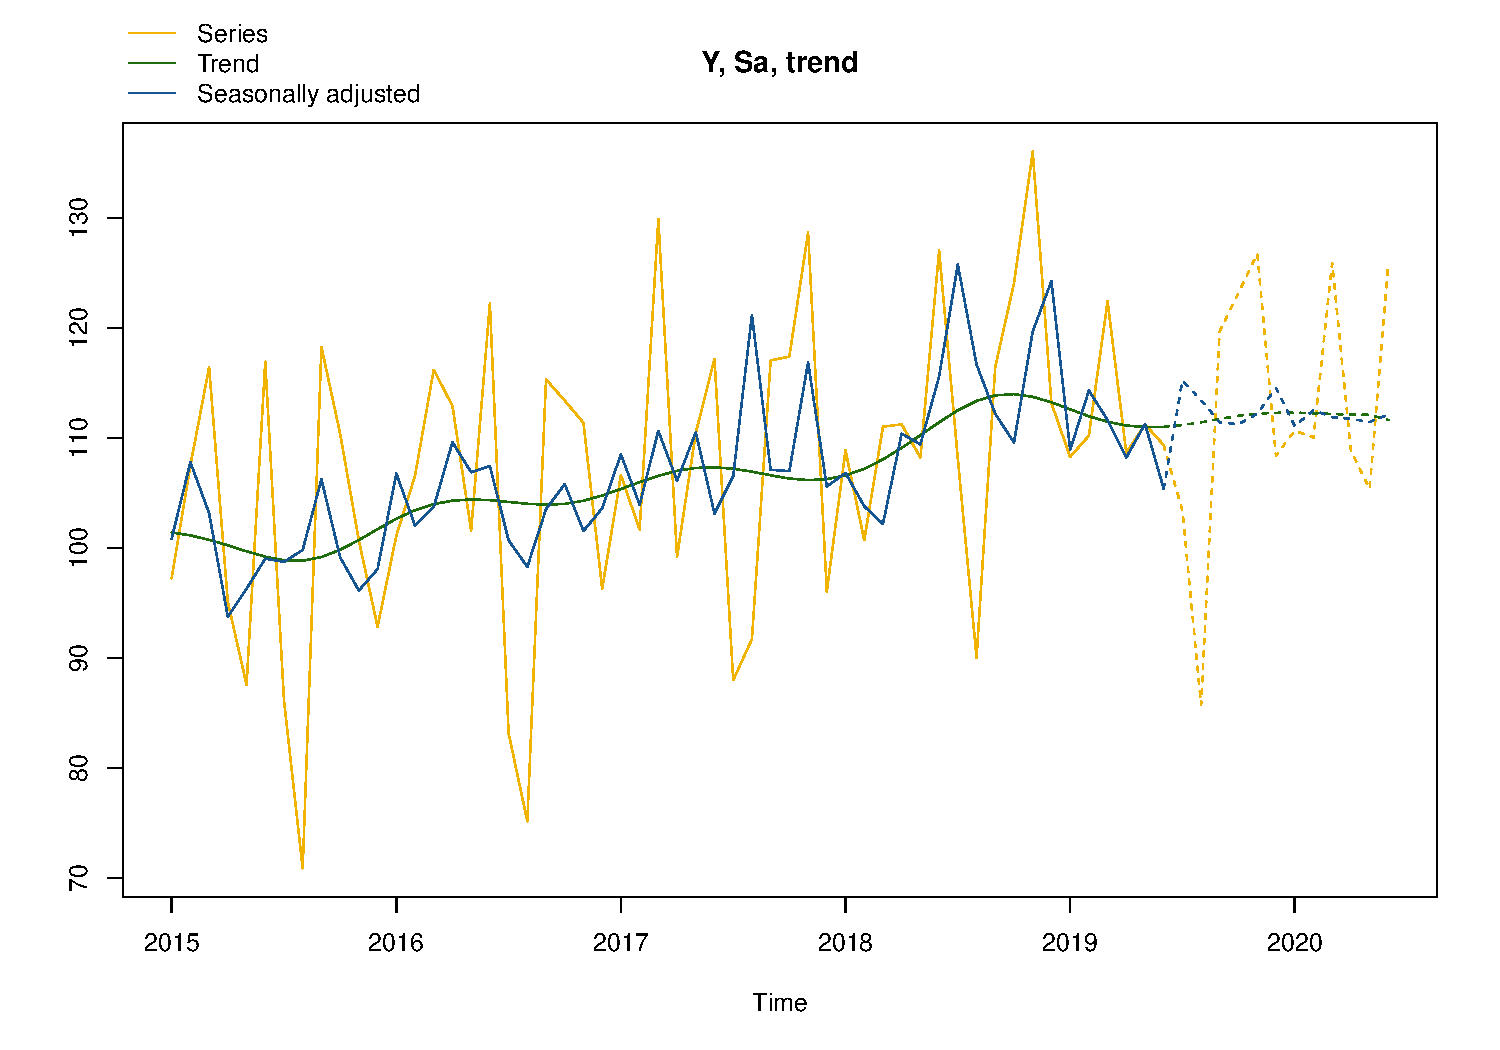
\includegraphics{img/markdown-unnamed-chunk-14-1} \end{center}

\begin{Shaded}
\begin{Highlighting}[]
\FunctionTok{plot}\NormalTok{(sa\_x13\_v2, }\AttributeTok{type=} \StringTok{"cal{-}seas{-}irr"}\NormalTok{,}\AttributeTok{first\_date =} \FunctionTok{c}\NormalTok{(}\DecValTok{2015}\NormalTok{, }\DecValTok{1}\NormalTok{))}
\end{Highlighting}
\end{Shaded}

\begin{center}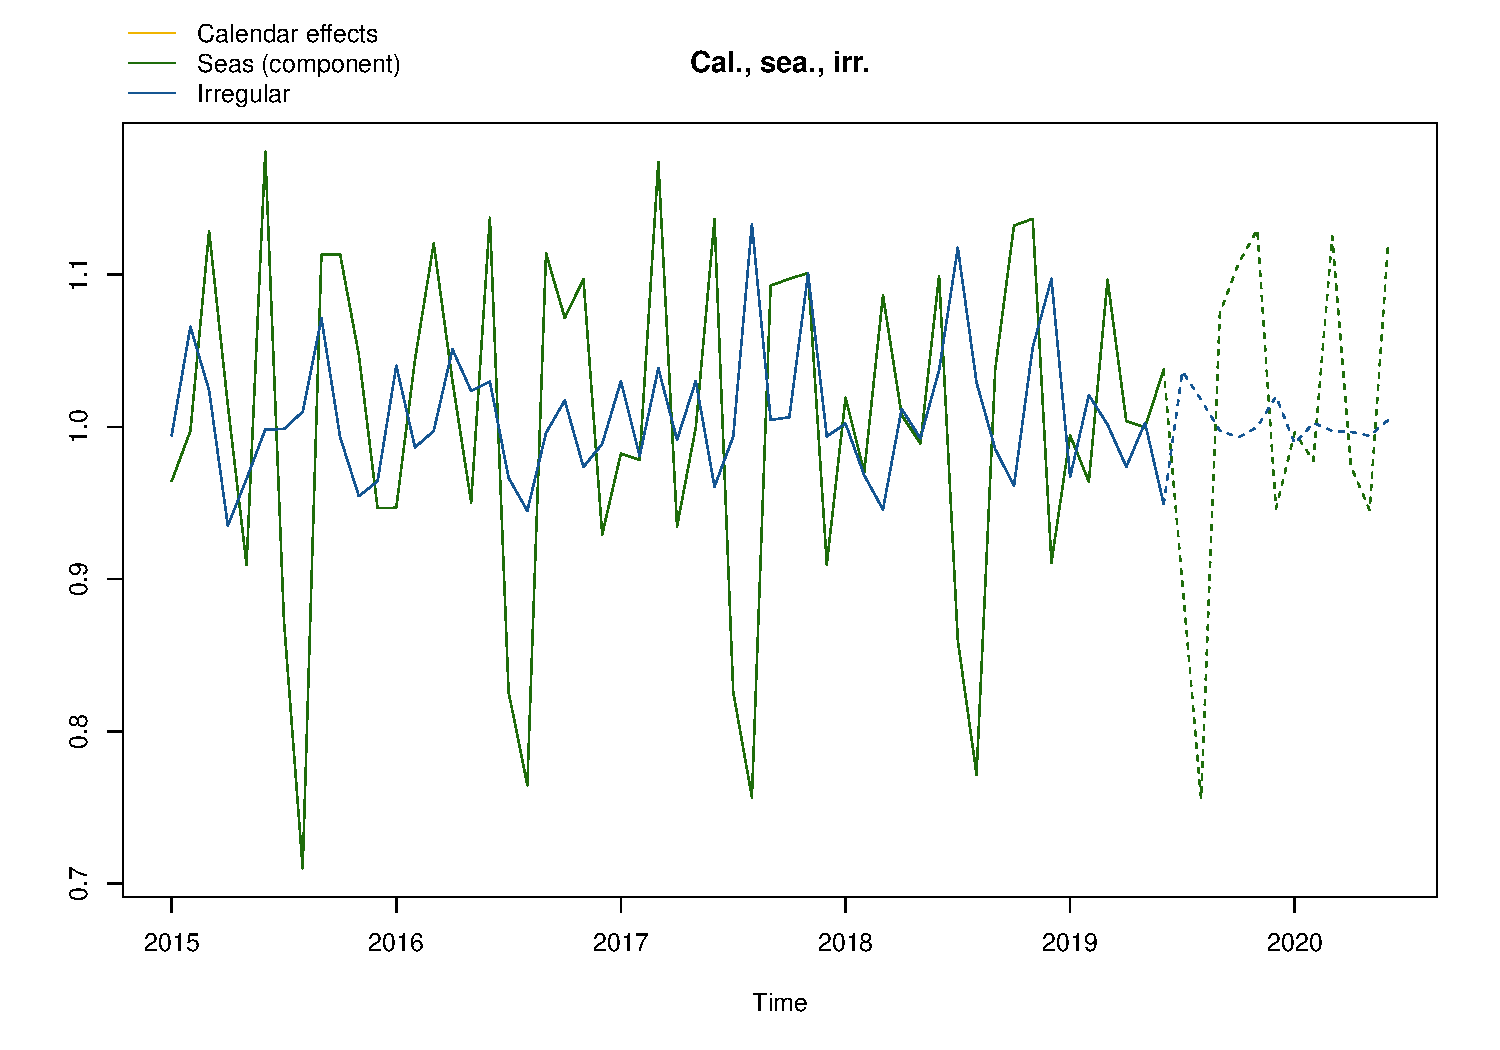
\includegraphics{img/markdown-unnamed-chunk-14-2} \end{center}

\begin{Shaded}
\begin{Highlighting}[]
\CommentTok{\# regarima}
\FunctionTok{layout}\NormalTok{(}\FunctionTok{matrix}\NormalTok{(}\DecValTok{1}\SpecialCharTok{:}\DecValTok{6}\NormalTok{, }\DecValTok{3}\NormalTok{, }\DecValTok{2}\NormalTok{));}\FunctionTok{plot}\NormalTok{(sa\_x13\_v2}\SpecialCharTok{$}\NormalTok{regarima,}\AttributeTok{ask =} \ConstantTok{FALSE}\NormalTok{)}
\end{Highlighting}
\end{Shaded}

\begin{center}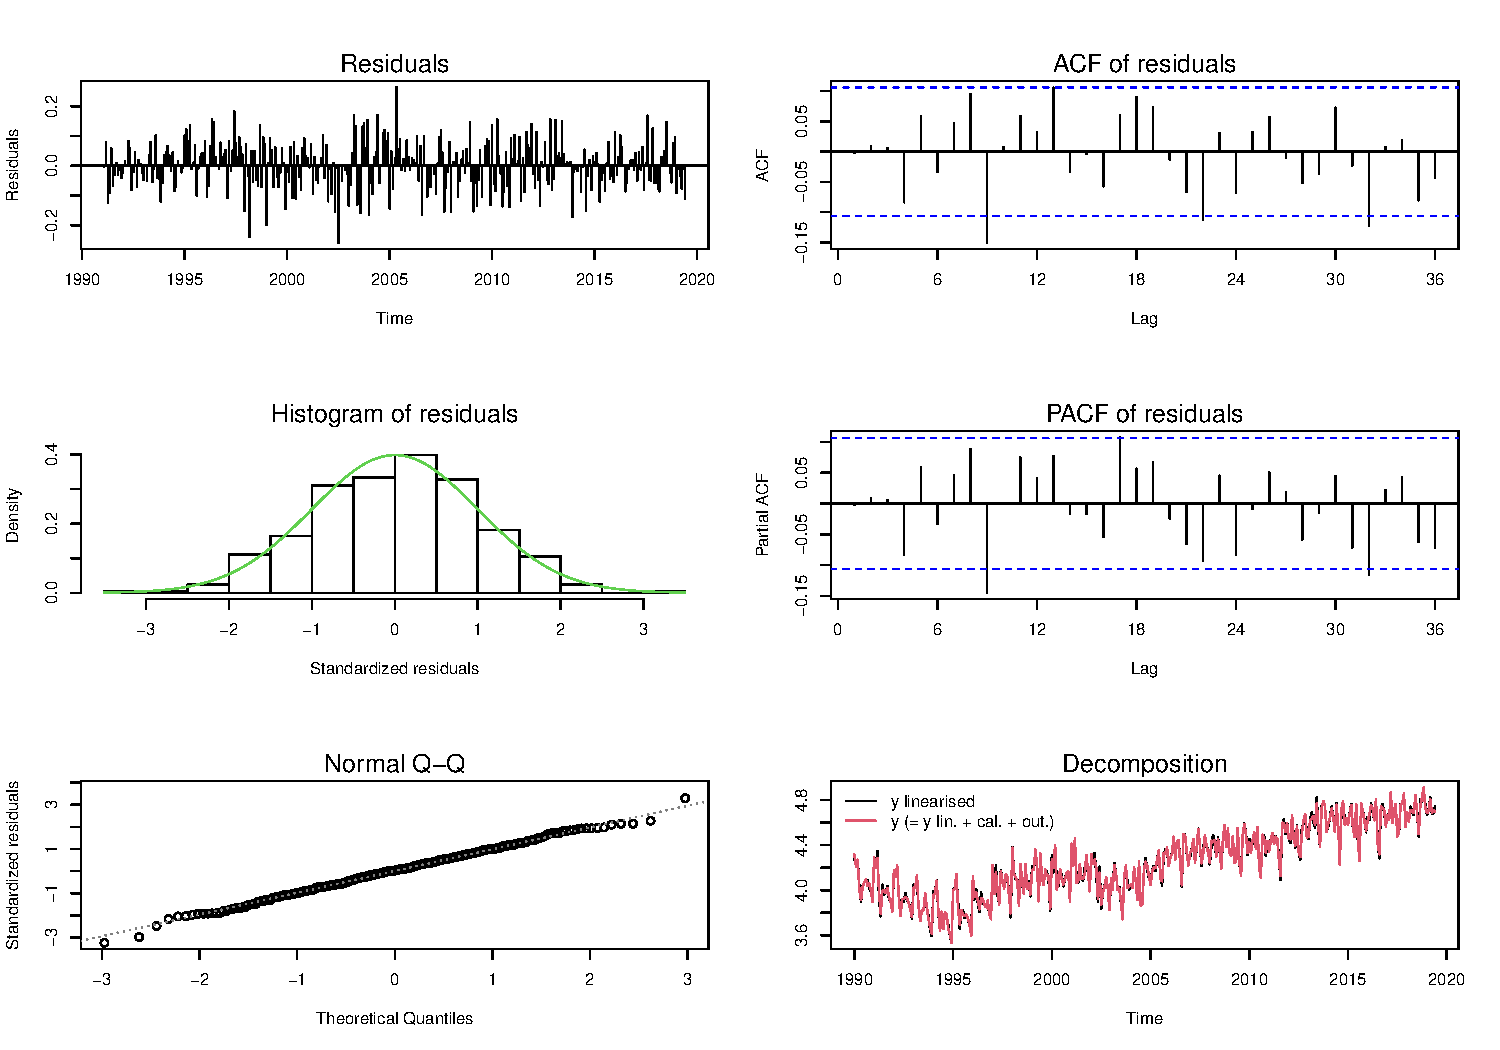
\includegraphics{img/markdown-unnamed-chunk-14-3} \end{center}

\begin{Shaded}
\begin{Highlighting}[]
\CommentTok{\# Plotting SI ratios  }
\FunctionTok{plot}\NormalTok{(sa\_x13\_v2}\SpecialCharTok{$}\NormalTok{decomposition, }\AttributeTok{first\_date =} \FunctionTok{c}\NormalTok{(}\DecValTok{2015}\NormalTok{,}\DecValTok{1}\NormalTok{))}
\end{Highlighting}
\end{Shaded}

\begin{center}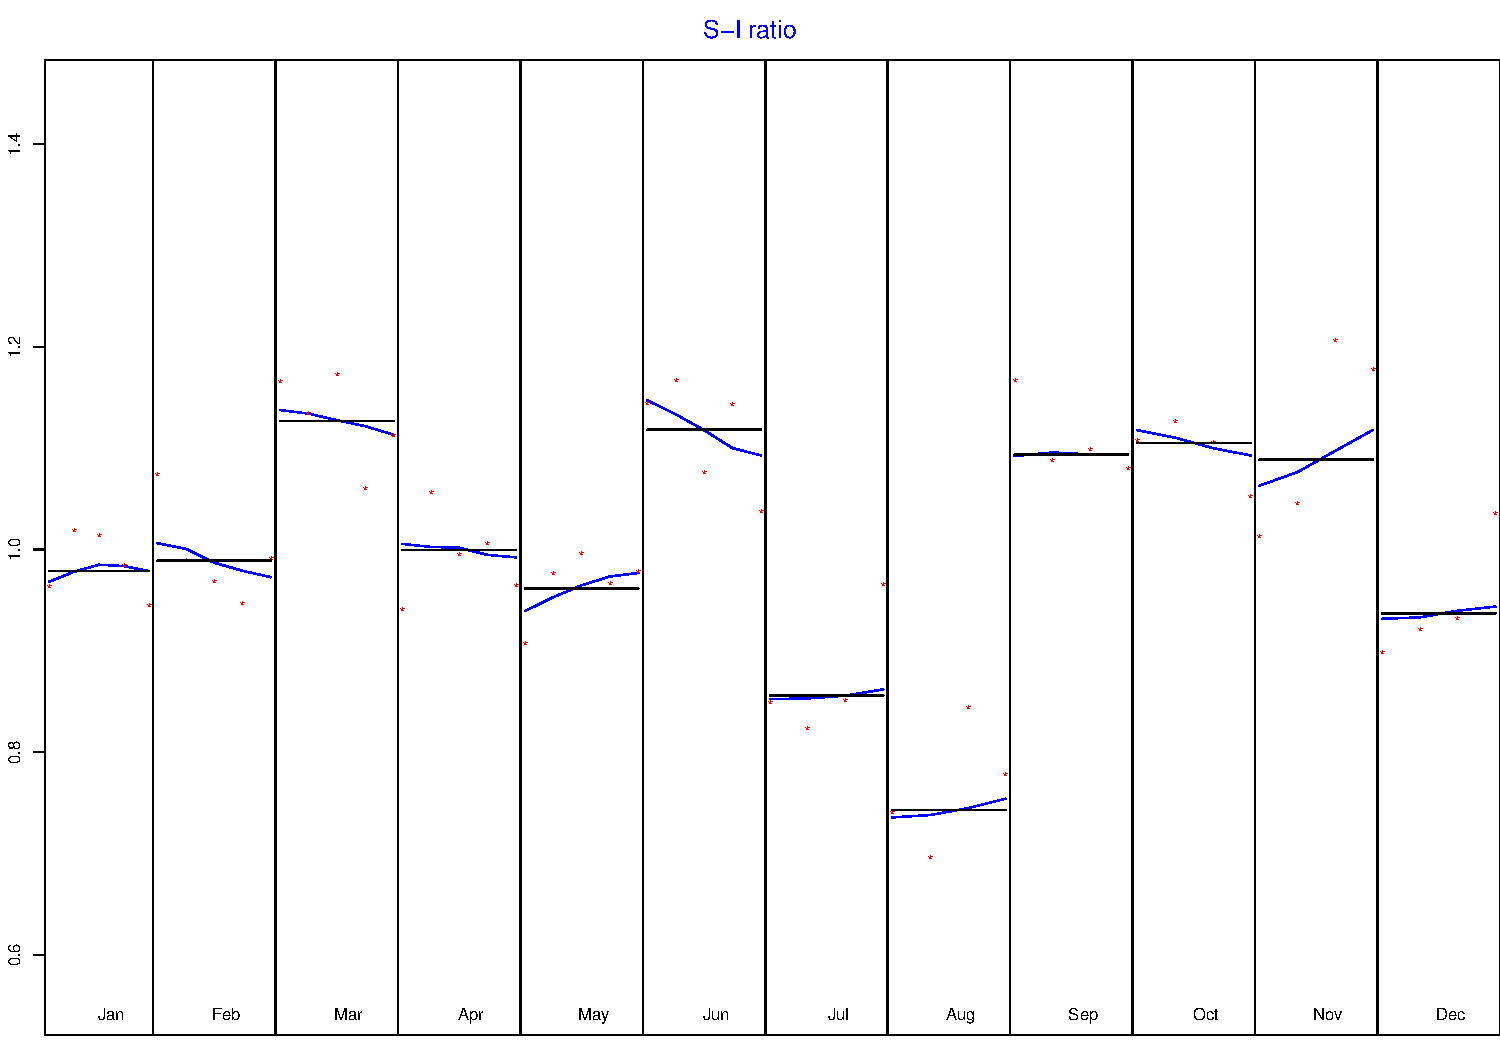
\includegraphics{img/markdown-unnamed-chunk-14-4} \end{center}
\end{frame}

\begin{frame}[fragile]{Plots and data visualisation (2/2)}
\protect\hypertarget{plots-and-data-visualisation-22}{}
In version 3 - final + NEW ``autoplot'' layout - regarima not available
(yet ?) - SI ratios + NEW ggplot layout

\begin{Shaded}
\begin{Highlighting}[]
\CommentTok{\# version 3}
\CommentTok{\# remotes::install\_github("AQLT/ggdemetra3",INSTALL\_opts = "{-}{-}no{-}multiarch")}
\CommentTok{\# library(ggdemetra3)}
\NormalTok{ggdemetra3}\SpecialCharTok{::}\FunctionTok{siratioplot}\NormalTok{(sa\_x13\_v3)}
\end{Highlighting}
\end{Shaded}

\begin{center}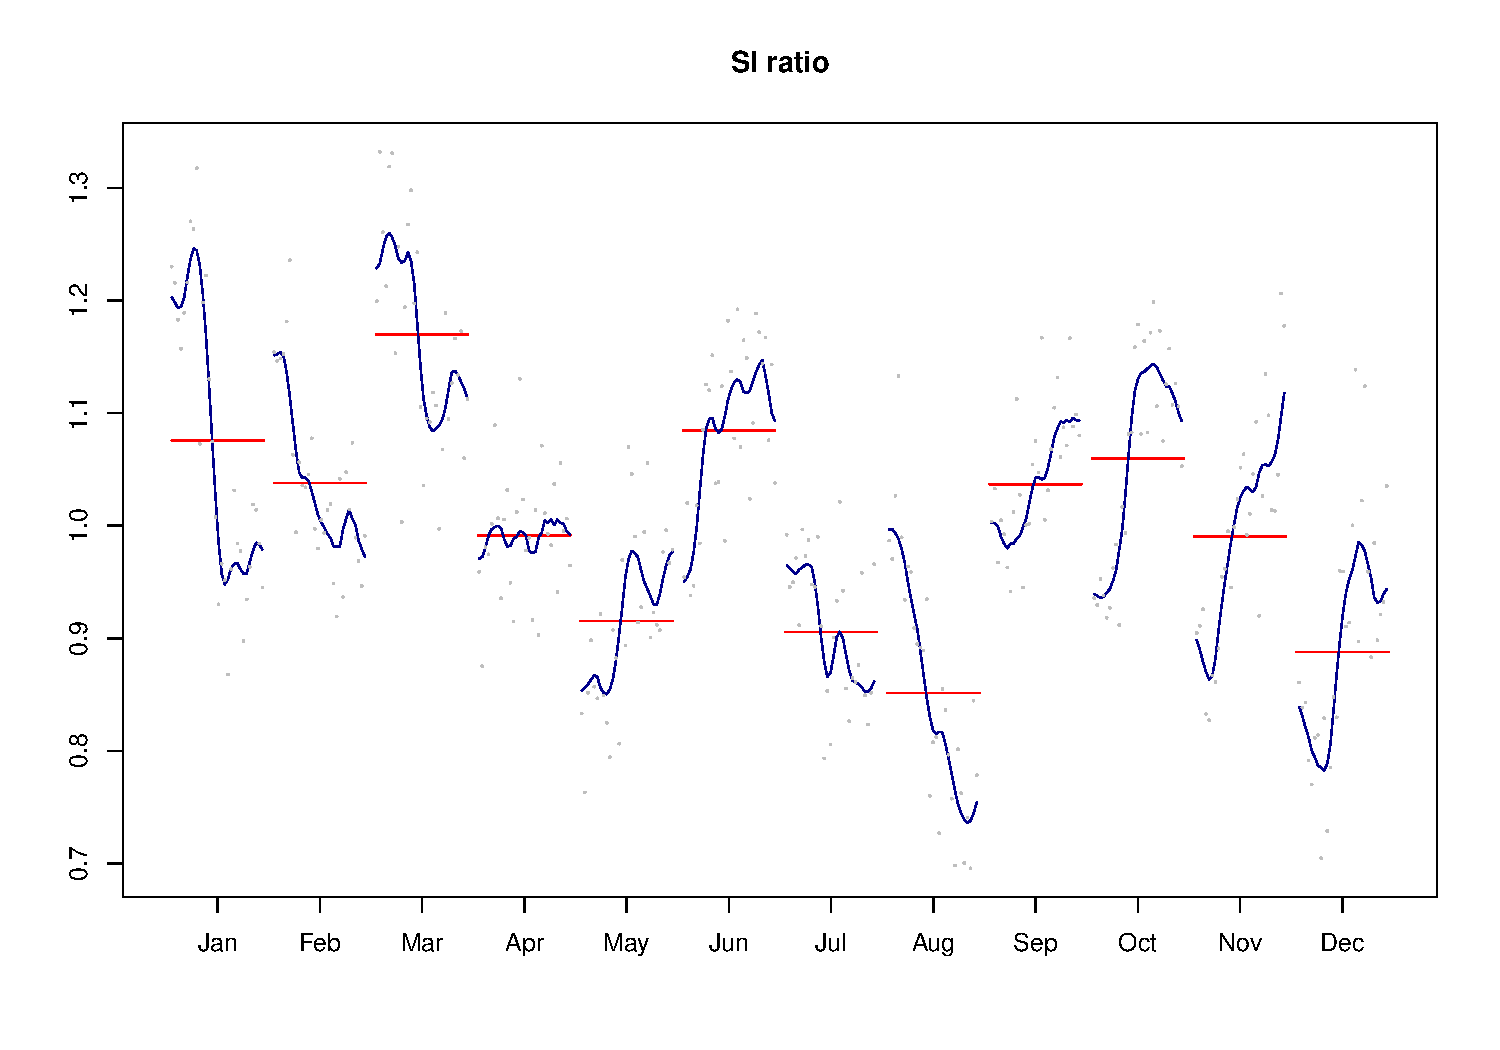
\includegraphics{img/markdown-unnamed-chunk-15-1} \end{center}

\begin{Shaded}
\begin{Highlighting}[]
\NormalTok{ggdemetra3}\SpecialCharTok{::}\FunctionTok{ggsiratioplot}\NormalTok{(sa\_x13\_v3)}
\end{Highlighting}
\end{Shaded}

\begin{center}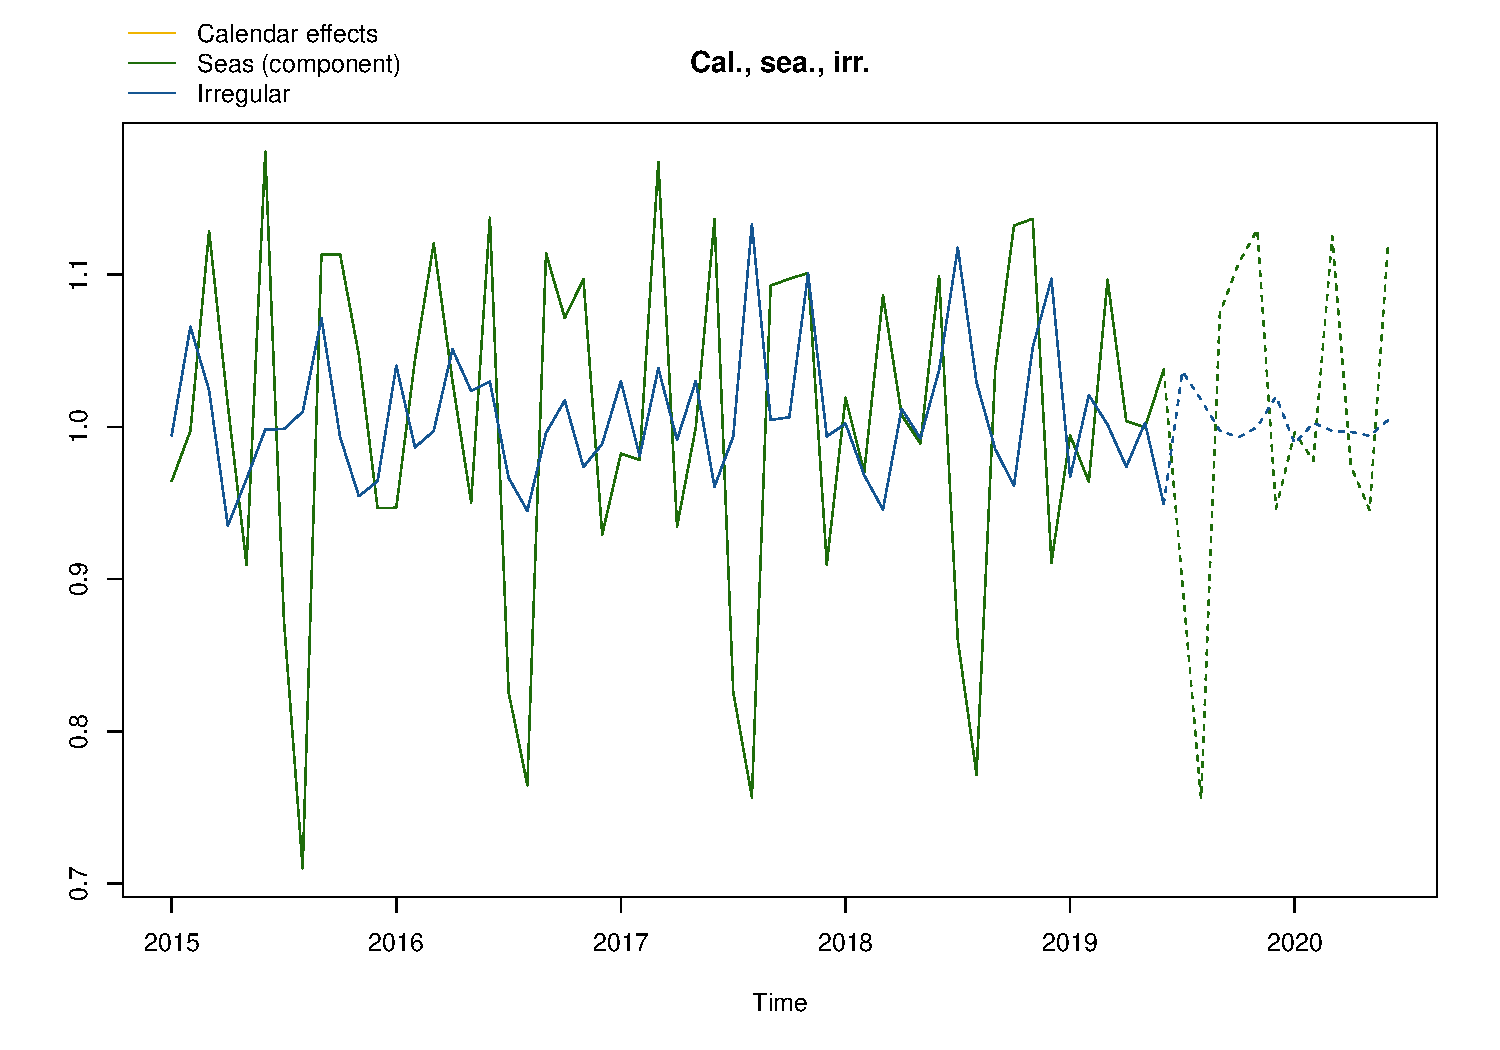
\includegraphics{img/markdown-unnamed-chunk-15-2} \end{center}

\begin{Shaded}
\begin{Highlighting}[]
\NormalTok{ggplot2}\SpecialCharTok{::}\FunctionTok{autoplot}\NormalTok{(sa\_x13\_v3)}
\end{Highlighting}
\end{Shaded}

\begin{center}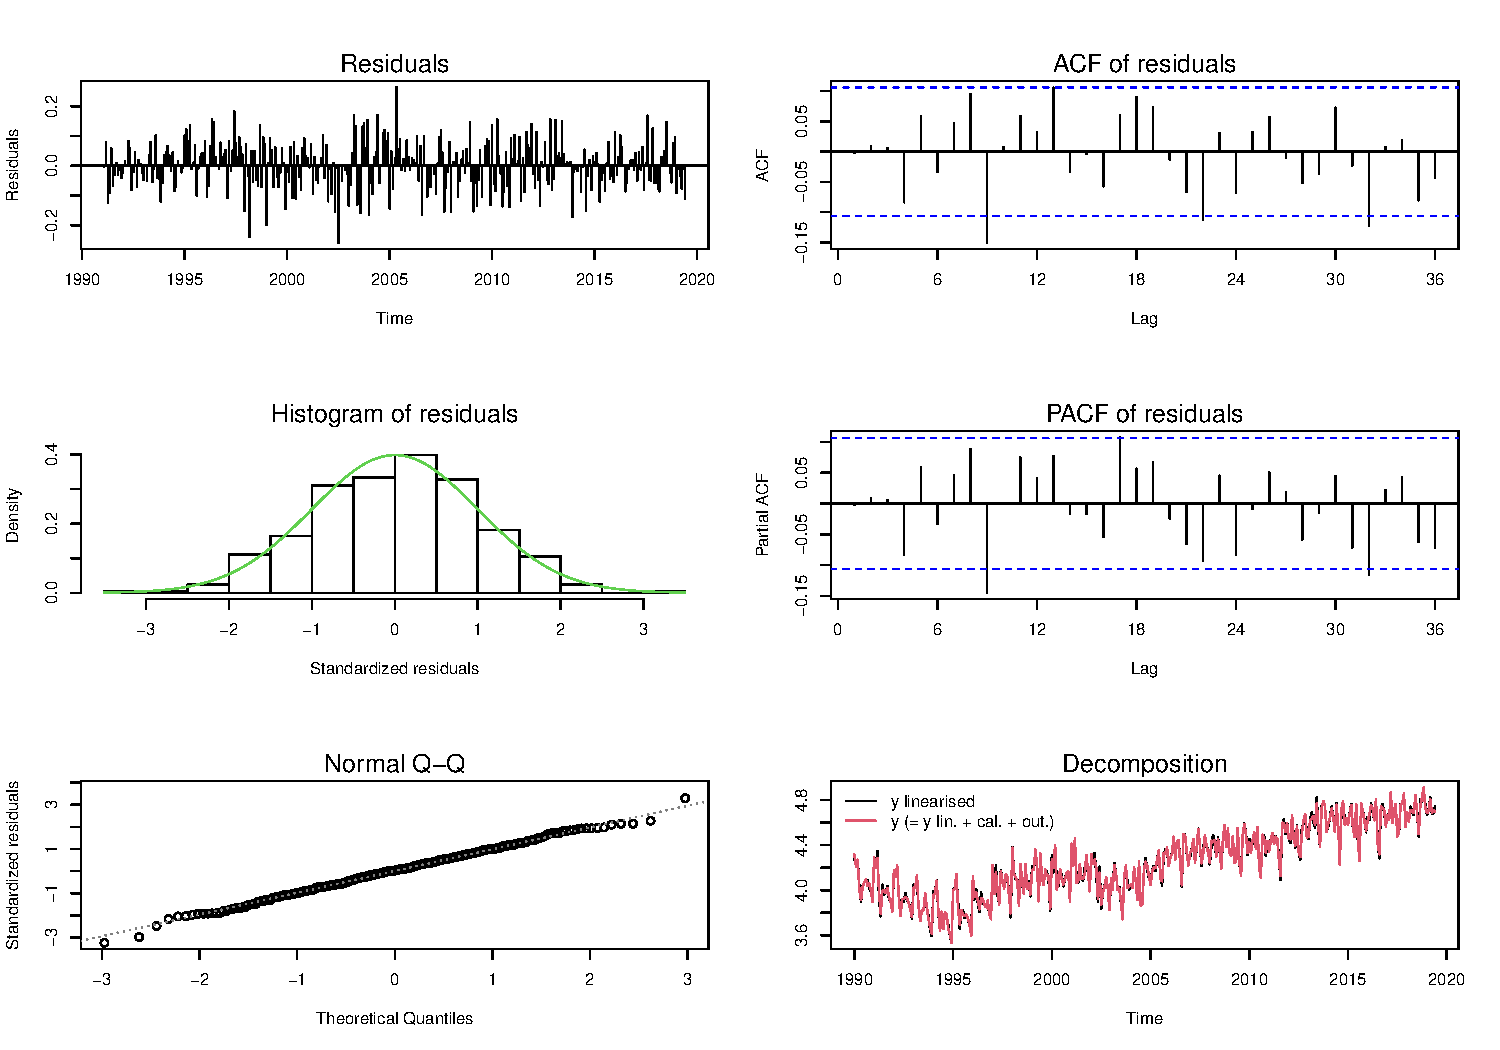
\includegraphics{img/markdown-unnamed-chunk-15-3} \end{center}
\end{frame}

\hypertarget{customizing-specifications}{%
\subsection{Customizing
specifications}\label{customizing-specifications}}

\begin{frame}{Customizing specifications: general steps}
\protect\hypertarget{customizing-specifications-general-steps}{}
To customize a specification you must - start with a valid
specification, usually one of the defaut specs (equivalent to cloning a
spec in GUI) - create a new spec - apply the new spec to a series

Some differences between v2 and v3
\end{frame}

\begin{frame}[fragile]{Customizing specifications: in version 2}
\protect\hypertarget{customizing-specifications-in-version-2}{}
Direct parameter modification as arguments of the spec function

\begin{Shaded}
\begin{Highlighting}[]
\CommentTok{\# version 2}
\CommentTok{\# changing estimation span, imposing additive model and adding user defined ouliers }
\CommentTok{\# first create a new spec modifying the previous one }
\NormalTok{spec\_1}\OtherTok{\textless{}{-}} \FunctionTok{x13\_spec}\NormalTok{(sa\_x13\_v2)}
\NormalTok{spec\_2}\OtherTok{\textless{}{-}} \FunctionTok{x13\_spec}\NormalTok{(spec\_1, }\AttributeTok{estimate.from =} \StringTok{"2004{-}01{-}01"}\NormalTok{,}
                  \AttributeTok{usrdef.outliersEnabled =} \ConstantTok{TRUE}\NormalTok{,}
                             \AttributeTok{usrdef.outliersType =} \FunctionTok{c}\NormalTok{(}\StringTok{"LS"}\NormalTok{, }\StringTok{"AO"}\NormalTok{),}
                             \AttributeTok{usrdef.outliersDate =} \FunctionTok{c}\NormalTok{(}\StringTok{"2008{-}10{-}01"}\NormalTok{, }\StringTok{"2018{-}01{-}01"}\NormalTok{),}
                             \AttributeTok{transform.function =} \StringTok{"None"}\NormalTok{) }\CommentTok{\# additive model}
\CommentTok{\# here the reg{-}arima model will be estimated from  "2004{-}01{-}01" }
\CommentTok{\# the decomposition will be run on the whole span }

\CommentTok{\# new sa processing}
\NormalTok{sa\_x13\_v2\_2}\OtherTok{\textless{}{-}}\NormalTok{RJDemetra}\SpecialCharTok{::}\FunctionTok{x13}\NormalTok{(serie\_brute,spec\_2)}
\NormalTok{sa\_x13\_v2\_2}\SpecialCharTok{$}\NormalTok{final}\SpecialCharTok{$}\NormalTok{series}
\end{Highlighting}
\end{Shaded}
\end{frame}

\begin{frame}[fragile]{Customizing specifications: in version 3}
\protect\hypertarget{customizing-specifications-in-version-3}{}
Use direct and specific \texttt{set\_} functions - for the preprocessing
step (functions defined in \texttt{rjd3modelling}):

\texttt{set\_arima()}, \texttt{set\_automodel()}, \texttt{set\_basic()},
\texttt{set\_easter()}, \texttt{set\_estimate()},
\texttt{set\_outlier()}, \texttt{set\_tradingdays()},
\texttt{set\_transform()}, \texttt{add\_outlier()} and
\texttt{remove\_outlier()}, \texttt{add\_ramp()} and
\texttt{remove\_ramp()}, \texttt{add\_usrdefvar()}

\begin{itemize}
\item
  for the decomposition step in X13 (function defined in
  \texttt{rjd3x13}): \texttt{set\_x11()}
\item
  for the decomposition step in Tramo-Seats (function defined in
  \texttt{rjd3tramoseats}): \texttt{set\_seats()}
\item
  for the benchmarking step (function defined in
  \texttt{rjd3modelling}): \texttt{set\_benchmarking()}
\end{itemize}

New v3 feature, same options available as in GUI.
\end{frame}

\begin{frame}[fragile]{Customizing specifications in version 3: example}
\protect\hypertarget{customizing-specifications-in-version-3-example}{}
\begin{Shaded}
\begin{Highlighting}[]
\DocumentationTok{\#\#\#\#\#\#\#\#\# spec custo in v3}
\CommentTok{\# start with default spec }
\NormalTok{spec\_1 }\OtherTok{=} \FunctionTok{spec\_x13\_default}\NormalTok{(}\StringTok{"RSA3"}\NormalTok{)}
\CommentTok{\# or start with existing spec (no extraction function needed)}
\NormalTok{spec\_1}\OtherTok{\textless{}{-}}\NormalTok{sa\_x13\_v3\_UD}\SpecialCharTok{$}\NormalTok{estimation\_spec}

\CommentTok{\# set a new spec}
\DocumentationTok{\#\# add outliers }
\NormalTok{spec\_2 }\OtherTok{=}\NormalTok{ rjd3modelling}\SpecialCharTok{::}\FunctionTok{add\_outlier}\NormalTok{(spec\_1,}
                  \AttributeTok{type =} \FunctionTok{c}\NormalTok{(}\StringTok{"AO"}\NormalTok{), }\FunctionTok{c}\NormalTok{(}\StringTok{"2015{-}01{-}01"}\NormalTok{, }\StringTok{"2010{-}01{-}01"}\NormalTok{))}
\DocumentationTok{\#\# set trading days}
\NormalTok{spec\_2}\OtherTok{\textless{}{-}}\NormalTok{rjd3modelling}\SpecialCharTok{::}\FunctionTok{set\_tradingdays}\NormalTok{(spec\_2,}
    \AttributeTok{option =} \StringTok{"workingdays"}\NormalTok{ )}
\CommentTok{\# set x11 options }
\NormalTok{spec\_2}\OtherTok{\textless{}{-}}\FunctionTok{set\_x11}\NormalTok{(spec\_2,}\AttributeTok{henderson.filter =} \DecValTok{13}\NormalTok{)}
\CommentTok{\# apply with \textasciigrave{}fast.x13\textasciigrave{} (results only)}
\FunctionTok{fast.x13}\NormalTok{(y,spec\_2)}
\end{Highlighting}
\end{Shaded}
\end{frame}

\begin{frame}{Adding user-defined regressors}
\protect\hypertarget{adding-user-defined-regressors}{}
In version 2: regressors added directly to the specification

In version 3: new notion of ``context'' an additionnal concept designed
to - -
\end{frame}

\begin{frame}[fragile]{Adding user-defined regressors in v2}
\protect\hypertarget{adding-user-defined-regressors-in-v2}{}
\begin{Shaded}
\begin{Highlighting}[]
\CommentTok{\# defining user defined trading days }
\NormalTok{spec\_4 }\OtherTok{\textless{}{-}} \FunctionTok{x13\_spec}\NormalTok{(spec\_1,}
\AttributeTok{tradingdays.option =} \StringTok{"UserDefined"}\NormalTok{,}
\AttributeTok{tradingdays.test =}\StringTok{"None"}\NormalTok{,}
\AttributeTok{usrdef.varEnabled =} \ConstantTok{TRUE}\NormalTok{,}
\CommentTok{\# the user defined variable will be assigned to the calendar component}
\AttributeTok{usrdef.varType=}\StringTok{"Calendar"}\NormalTok{,}
\AttributeTok{usrdef.var=}\NormalTok{td\_regs ) }\CommentTok{\# regressors have to be a single or multiple TS }
\CommentTok{\# new sa processing}
\NormalTok{sa\_x13\_v2\_4}\OtherTok{\textless{}{-}}\FunctionTok{x13}\NormalTok{(serie\_brute,spec\_4)}
\CommentTok{\# user defined intervention variable  }
\NormalTok{spec\_5 }\OtherTok{\textless{}{-}} \FunctionTok{x13\_spec}\NormalTok{(spec\_1,}
                   \AttributeTok{usrdef.varEnabled =} \ConstantTok{TRUE}\NormalTok{,}
                   \CommentTok{\# the user defined variable will be assigned to the trend component}
                   \AttributeTok{usrdef.varType=}\StringTok{"Trend"}\NormalTok{,}
                   \AttributeTok{usrdef.var=}\NormalTok{x ) }\CommentTok{\# x has to to be a single or multiple TS }
\CommentTok{\# new sa processing}
\NormalTok{sa\_x13\_v2\_5}\OtherTok{\textless{}{-}}\FunctionTok{x13}\NormalTok{(serie\_brute,spec\_5)}
\end{Highlighting}
\end{Shaded}
\end{frame}

\begin{frame}[fragile]{Adding user-defined regressors in version 3}
\protect\hypertarget{adding-user-defined-regressors-in-version-3}{}
\begin{Shaded}
\begin{Highlighting}[]
\CommentTok{\# defining user defined trading days }
\NormalTok{td\_reg1}\OtherTok{\textless{}{-}}\NormalTok{ rjd3modelling}\SpecialCharTok{::}\FunctionTok{td}\NormalTok{(}\DecValTok{12}\NormalTok{, }\AttributeTok{start=}\FunctionTok{start}\NormalTok{(y\_raw),}\AttributeTok{length =} \FunctionTok{length}\NormalTok{(y\_raw),}\AttributeTok{groups =} \FunctionTok{c}\NormalTok{(}\DecValTok{1}\NormalTok{,}\DecValTok{1}\NormalTok{,}\DecValTok{1}\NormalTok{,}\DecValTok{1}\NormalTok{,}\DecValTok{1}\NormalTok{,}\DecValTok{0}\NormalTok{,}\DecValTok{0}\NormalTok{))}

\NormalTok{context}\OtherTok{\textless{}{-}}\NormalTok{rjd3modelling}\SpecialCharTok{::}\FunctionTok{modelling\_context}\NormalTok{(}\AttributeTok{variables=}\FunctionTok{list}\NormalTok{(}\AttributeTok{a=}\NormalTok{xvar))}

\NormalTok{spec }\OtherTok{\textless{}{-}}\NormalTok{ rjd3x13}\SpecialCharTok{::}\FunctionTok{spec\_regarima\_default}\NormalTok{(}\AttributeTok{name =} \StringTok{"rg3"}\NormalTok{) }\SpecialCharTok{|\textgreater{}}
\NormalTok{  rjd3modelling}\SpecialCharTok{::}\FunctionTok{add\_usrdefvar}\NormalTok{(}\AttributeTok{id =} \StringTok{"r.a"}\NormalTok{)}

\NormalTok{reg\_a\_estimation}\OtherTok{\textless{}{-}}\NormalTok{rjd3x13}\SpecialCharTok{::}\FunctionTok{regarima}\NormalTok{(}\FunctionTok{window}\NormalTok{(ts, }\AttributeTok{start=}\DecValTok{1985}\NormalTok{, }\AttributeTok{end=}\DecValTok{2013}\NormalTok{),sp,}\AttributeTok{context =}\NormalTok{ context)}

\CommentTok{\# if user\_def variable to tren d? how to chose component ?}
\CommentTok{\# regressors have to be added one by one }
\end{Highlighting}
\end{Shaded}
\end{frame}

\hypertarget{refreshing-data}{%
\subsection{Refreshing data}\label{refreshing-data}}

\begin{frame}[fragile]{Estimation\_spec vs result\_spec (1/2)}
\protect\hypertarget{estimation_spec-vs-result_spec-12}{}
Possibility of refreshing data is new feature of version 3.

In the ``sa\_model'' object generated by the estimation process:

\begin{itemize}
\item
  new handling of spec (no extraction needed as separated)
\item
  notion of

  \begin{itemize}
  \tightlist
  \item
    estimation spec (domain spec): set of customizable constraints
  \end{itemize}
\end{itemize}

\footnotesize

\begin{Shaded}
\begin{Highlighting}[]
\NormalTok{sa\_x13\_v3}\SpecialCharTok{$}\NormalTok{estimation\_spec}\SpecialCharTok{$}\NormalTok{regarima}\SpecialCharTok{$}\NormalTok{arima}
\end{Highlighting}
\end{Shaded}

\begin{verbatim}
- result spec (or point spec)
\end{verbatim}

\footnotesize

\begin{Shaded}
\begin{Highlighting}[]
\NormalTok{sa\_x13\_v3}\SpecialCharTok{$}\NormalTok{result\_spec}\SpecialCharTok{$}\NormalTok{regarima}\SpecialCharTok{$}\NormalTok{arima}
\end{Highlighting}
\end{Shaded}
\end{frame}

\begin{frame}{Estimation\_spec vs result\_spec}
\protect\hypertarget{estimation_spec-vs-result_spec}{}
\begin{itemize}
\tightlist
\item
  in v2 could only retrieve a (point) result\_spec (extracted with
  x13\_spec)
\item
  in v3 your are able to restimate the result spec inside the domain
  (estimation spec) freeing constriants on some parameters : just like
  in GUI
\end{itemize}
\end{frame}

\begin{frame}[fragile]{Steps for refreshing data}
\protect\hypertarget{steps-for-refreshing-data}{}
\begin{Shaded}
\begin{Highlighting}[]
\NormalTok{current\_result\_spec}\OtherTok{\textless{}{-}}\NormalTok{sa\_x13\_v3}\SpecialCharTok{$}\NormalTok{result\_spec}
\NormalTok{current\_domain\_spec}\OtherTok{\textless{}{-}}\NormalTok{sa\_x13\_v3}\SpecialCharTok{$}\NormalTok{estimation\_spec}

\CommentTok{\# generate NEW spec for refresh }
\NormalTok{refreshed\_spec}\OtherTok{\textless{}{-}}\FunctionTok{x13.refresh}\NormalTok{(current\_spec, }\CommentTok{\# point spec to be refreshed}
\NormalTok{            current\_domain\_spec, }\CommentTok{\#domain spec (set of constraints)}
            \AttributeTok{policy =} \StringTok{"Outliers"}\NormalTok{,}
            \AttributeTok{period =} \DecValTok{12}\NormalTok{, }\CommentTok{\# monthly series}
            \AttributeTok{start =} \StringTok{"2017{-}01{-}01"}\NormalTok{,}
            \AttributeTok{end =} \ConstantTok{NULL}\NormalTok{)}

\CommentTok{\# apply the new spec on new data : y\_new= y\_raw + 3 months}
\NormalTok{sa\_x13\_v3\_refresh}\OtherTok{\textless{}{-}}\FunctionTok{x13}\NormalTok{(y\_new,refreshed\_spec)}
\CommentTok{\# what will be the domain spec here ?}
\CommentTok{\# domain spec = point spec ?}
\end{Highlighting}
\end{Shaded}

\begin{itemize}
\tightlist
\item
  Outliers identiication : more flaxible the last ouliers or all
  outleirs in v2, here the span can be customized (Warning: x13.refresh
  hasn't been thouroughly tested yet)
\end{itemize}
\end{frame}

\begin{frame}{Refresh Policies}
\protect\hypertarget{refresh-policies}{}
\begin{itemize}
\tightlist
\item
  ``FreeParameters'',
\item
  ``Complete'':
\item
  ``Outliers\_StochasticComponent'',
\item
  ``Outliers'',
\item
  ``FixedParameters'',
\item
  ``FixedAutoRegressiveParameters'',
\item
  ``Fixed'',
\end{itemize}
\end{frame}

\begin{frame}{User-defined parameters: summary}
\protect\hypertarget{user-defined-parameters-summary}{}
\begin{itemize}
\tightlist
\item
  what's new ?
\item
  whats's missing ?
\end{itemize}
\end{frame}

\hypertarget{sa-of-high-frequency-data}{%
\section{SA of High-Frequency data}\label{sa-of-high-frequency-data}}

\begin{frame}{SA of High-Frequency data (1/2)}
\protect\hypertarget{sa-of-high-frequency-data-12}{}
Specificity: high-frequency data can display multiple and non integer
periodicities:

For example a daily serie might display 3 periodicities: - weekly
(\(p=7\)): Mondays are alike and different from Sundays (DOW) -
intra-monthly (\(p=30.44\)): the last days of each month are different
from the first ones (DOM) - yearly (\(p=365.25\)): from on year to
another the 15th of June are alike, summer days are alike (DOY)

Two classes of solutions: - round periodicities (might involve imputing
data) (extended STL,..) - use approximations for fractional backshift
powers (extended X13-Arima and Tramo-Seats)
\end{frame}

\begin{frame}{SA of High-Frequency data (2/2)}
\protect\hypertarget{sa-of-high-frequency-data-22}{}
Specific tools: rjd3highfreq and rjd3stl (version 3) (version 2 :
rjdhighfreq)

Different data format: numeric vectors (and NOT TS objects)

\begin{itemize}
\item
  linerarization with fractionnal airline model (correction for calendar
  effects and outlier detection)
\item
  iterative decomposition (extrended X-11 and Seats) starting with the
  highest frequency
\end{itemize}

See presentation about \{rjd3highfreq\} (Webinar GitHub Repo)
\end{frame}

\begin{frame}[fragile]{Linearization: code template}
\protect\hypertarget{linearization-code-template}{}
\footnotesize

\begin{Shaded}
\begin{Highlighting}[]
\NormalTok{rjd3highfreq}\SpecialCharTok{::}\NormalTok{fractionalAirlineEstimation}
\NormalTok{                        (df\_daily}\SpecialCharTok{$}\NormalTok{log\_births, }\CommentTok{\# here series in log}
                \AttributeTok{x =}\NormalTok{ q, }\CommentTok{\# q= calendar}
                \AttributeTok{periods =} \DecValTok{7}\NormalTok{, }\CommentTok{\# approx  c(7,365.25)}
                \AttributeTok{ndiff =} \DecValTok{2}\NormalTok{, }\AttributeTok{ar =} \ConstantTok{FALSE}\NormalTok{, }\AttributeTok{mean =} \ConstantTok{FALSE}\NormalTok{,}
                \AttributeTok{outliers =} \FunctionTok{c}\NormalTok{(}\StringTok{"ao"}\NormalTok{,}\StringTok{"wo"}\NormalTok{), }
                \CommentTok{\# WO compensation, LS not relevant here }
                \AttributeTok{criticalValue =} \DecValTok{0}\NormalTok{, }\CommentTok{\# computed in the algorithm}
                \AttributeTok{precision =} \FloatTok{1e{-}9}\NormalTok{, }\AttributeTok{approximateHessian =} \ConstantTok{TRUE}\NormalTok{)}
                    
\CommentTok{\# calendar regressors can be defined with the \{rjd3modelling\} package }
\end{Highlighting}
\end{Shaded}

See \{rjd3highfreq\} help pages
\end{frame}

\begin{frame}[fragile]{Decomposition with extended X-11: code template}
\protect\hypertarget{decomposition-with-extended-x-11-code-template}{}
\footnotesize

\begin{Shaded}
\begin{Highlighting}[]
\CommentTok{\#step 1: p=7}
\NormalTok{x11.dow}\OtherTok{\textless{}{-}}\NormalTok{rjd3highfreq}\SpecialCharTok{::}\FunctionTok{x11}\NormalTok{(}\FunctionTok{exp}\NormalTok{(pre.mult}\SpecialCharTok{$}\NormalTok{model}\SpecialCharTok{$}\NormalTok{linearized),}
        \AttributeTok{period =} \DecValTok{7}\NormalTok{,                 }\CommentTok{\# DOW pattern}
        \AttributeTok{mul =} \ConstantTok{TRUE}\NormalTok{,                              }
        \AttributeTok{trend.horizon =} \DecValTok{9}\NormalTok{,  }\CommentTok{\# 1/2 Filter length : not too long vs p}
        \AttributeTok{trend.degree =} \DecValTok{3}\NormalTok{,                         }\CommentTok{\# Polynomial degree}
        \AttributeTok{trend.kernel =} \StringTok{"Henderson"}\NormalTok{,               }\CommentTok{\# Kernel function}
        \AttributeTok{trend.asymmetric =} \StringTok{"CutAndNormalize"}\NormalTok{,     }\CommentTok{\# Truncation method}
        \AttributeTok{seas.s0 =} \StringTok{"S3X9"}\NormalTok{, }\AttributeTok{seas.s1 =} \StringTok{"S3X9"}\NormalTok{,       }\CommentTok{\# Seasonal filters}
        \AttributeTok{extreme.lsig =} \FloatTok{1.5}\NormalTok{, }\AttributeTok{extreme.usig =} \FloatTok{2.5}\NormalTok{)   }\CommentTok{\# Sigma{-}limits}
\CommentTok{\#step 2: p=365.25}
\NormalTok{x11.doy}\OtherTok{\textless{}{-}}\NormalTok{ rjd3highfreq}\SpecialCharTok{::}\FunctionTok{x11}\NormalTok{(x11.dow}\SpecialCharTok{$}\NormalTok{decomposition}\SpecialCharTok{$}\NormalTok{sa,  }\CommentTok{\# previous sa}
                    \AttributeTok{period =} \FloatTok{365.2425}\NormalTok{,         }\CommentTok{\# DOY pattern}
                    \AttributeTok{mul =} \ConstantTok{TRUE}\NormalTok{) }\CommentTok{\#other parameters skipped here}
\end{Highlighting}
\end{Shaded}

See \{rjd3highfreq\} help pages for more details
\end{frame}

\begin{frame}[fragile]{Decomposition with extended Seats: code template}
\protect\hypertarget{decomposition-with-extended-seats-code-template}{}
\footnotesize

\begin{Shaded}
\begin{Highlighting}[]
\CommentTok{\#step 1: p=7}
\CommentTok{\#step 2: p=365.25}
\NormalTok{amb.doy }\OtherTok{\textless{}{-}}\NormalTok{ rjd3highfreq}\SpecialCharTok{::}\FunctionTok{fractionalAirlineDecomposition}\NormalTok{(}
\NormalTok{  amb.dow}\SpecialCharTok{$}\NormalTok{decomposition}\SpecialCharTok{$}\NormalTok{sa,  }\CommentTok{\# DOW{-}adjusted linearised data}
  \AttributeTok{period =} \FloatTok{365.2425}\NormalTok{,         }\CommentTok{\# DOY pattern}
  \AttributeTok{sn =} \ConstantTok{FALSE}\NormalTok{,                }\CommentTok{\# Signal (SA){-}noise decomposition }
  \AttributeTok{stde =} \ConstantTok{FALSE}\NormalTok{,              }\CommentTok{\# Compute standard deviations}
  \AttributeTok{nbcasts =} \DecValTok{0}\NormalTok{, }\AttributeTok{nfcasts =} \DecValTok{0}\NormalTok{)  }\CommentTok{\# Numbers of back{-} and forecasts}
\end{Highlighting}
\end{Shaded}

See \{rjd3highfreq\} help pages for more details
\end{frame}

\hypertarget{generating-user-defined-auxilary-variables}{%
\section{Generating User-defined auxilary
variables}\label{generating-user-defined-auxilary-variables}}

\hypertarget{calendars}{%
\subsection{calendars}\label{calendars}}

\begin{frame}{calendars}
\protect\hypertarget{calendars-1}{}
New features of version 3:

\begin{itemize}
\item
  generating calendars in R (see GUI function in v2)
\item
  generating calendars regressors

  \begin{itemize}
  \tightlist
  \item
    raw number of days or contrasts
  \item
    long term mean correction or not
  \item
    user-defined groups of days
  \item
    user-defined contrast days (associated with holidays)
  \end{itemize}
\end{itemize}

can be done with \{rjd3modelling\} package
\end{frame}

\begin{frame}[fragile]{Creation of a specific calendar}
\protect\hypertarget{creation-of-a-specific-calendar}{}
\footnotesize

\begin{Shaded}
\begin{Highlighting}[]
\FunctionTok{library}\NormalTok{(rjd3modelling)}
\NormalTok{fr\_cal }\OtherTok{\textless{}{-}} \FunctionTok{calendar.new}\NormalTok{()}
\FunctionTok{calendar.holiday}\NormalTok{(fr\_cal, }\StringTok{"NEWYEAR"}\NormalTok{)}
\FunctionTok{calendar.holiday}\NormalTok{(fr\_cal, }\StringTok{"EASTERMONDAY"}\NormalTok{)}
\FunctionTok{calendar.holiday}\NormalTok{(fr\_cal, }\StringTok{"MAYDAY"}\NormalTok{)}
\FunctionTok{calendar.fixedday}\NormalTok{(fr\_cal, }\AttributeTok{month =} \DecValTok{5}\NormalTok{, }\AttributeTok{day =} \DecValTok{8}\NormalTok{,}
                  \AttributeTok{start =} \StringTok{"1953{-}03{-}20"}\NormalTok{)}
\CommentTok{\# calendar.holiday(fr\_cal, "WHITMONDAY") \# Equivalent to:}
\FunctionTok{calendar.easter}\NormalTok{(fr\_cal, }\AttributeTok{offset =} \DecValTok{61}\NormalTok{)}

\FunctionTok{calendar.fixedday}\NormalTok{(fr\_cal, }\AttributeTok{month =} \DecValTok{7}\NormalTok{, }\AttributeTok{day =} \DecValTok{14}\NormalTok{)}
\CommentTok{\# calendar.holiday(fr\_cal, "ASSUMPTION")}
\FunctionTok{calendar.easter}\NormalTok{(fr\_cal, }\AttributeTok{offset =} \DecValTok{61}\NormalTok{)}
\FunctionTok{calendar.holiday}\NormalTok{(fr\_cal, }\StringTok{"ALLSAINTSDAY"}\NormalTok{)}
\FunctionTok{calendar.holiday}\NormalTok{(fr\_cal, }\StringTok{"ARMISTICE"}\NormalTok{)}
\FunctionTok{calendar.holiday}\NormalTok{(fr\_cal, }\StringTok{"CHRISTMAS"}\NormalTok{)}
\end{Highlighting}
\end{Shaded}
\end{frame}

\begin{frame}[fragile,allowframebreaks]{Creation of a associated
regressors}
\protect\hypertarget{creation-of-a-associated-regressors}{}
Use \texttt{holidays()} to get the days of the holidays and
\texttt{htd()} to get the trading days regressors

\footnotesize

\begin{Shaded}
\begin{Highlighting}[]
\FunctionTok{holidays}\NormalTok{(fr\_cal, }\StringTok{"2020{-}12{-}24"}\NormalTok{, }\DecValTok{10}\NormalTok{,}\AttributeTok{single =}\NormalTok{ T)}
\end{Highlighting}
\end{Shaded}

\begin{verbatim}
##            [,1]
## 2020-12-24    0
## 2020-12-25    1
## 2020-12-26    0
## 2020-12-27    0
## 2020-12-28    0
## 2020-12-29    0
## 2020-12-30    0
## 2020-12-31    0
## 2021-01-01    1
## 2021-01-02    0
\end{verbatim}

\begin{Shaded}
\begin{Highlighting}[]
\NormalTok{s }\OtherTok{=} \FunctionTok{ts}\NormalTok{(}\DecValTok{0}\NormalTok{, }\AttributeTok{start =} \DecValTok{2020}\NormalTok{, }\AttributeTok{end =} \FunctionTok{c}\NormalTok{(}\DecValTok{2020}\NormalTok{, }\DecValTok{11}\NormalTok{), }\AttributeTok{frequency =} \DecValTok{12}\NormalTok{)}
\CommentTok{\# Trading{-}days regressors (each day has a different effect, sunday as contrasts)}
\NormalTok{td\_reg }\OtherTok{\textless{}{-}} \FunctionTok{htd}\NormalTok{(fr\_cal, }\AttributeTok{s =}\NormalTok{ s, }\AttributeTok{groups =} \FunctionTok{c}\NormalTok{(}\DecValTok{1}\NormalTok{, }\DecValTok{2}\NormalTok{, }\DecValTok{3}\NormalTok{, }\DecValTok{4}\NormalTok{, }\DecValTok{5}\NormalTok{, }\DecValTok{6}\NormalTok{, }\DecValTok{0}\NormalTok{))}
\CommentTok{\# Working{-}days regressors (Monday = ... = Friday; Saturday = Sunday = contrasts)}
\NormalTok{wd\_reg }\OtherTok{\textless{}{-}} \FunctionTok{htd}\NormalTok{(fr\_cal, }\AttributeTok{s =}\NormalTok{ s, }\AttributeTok{groups =} \FunctionTok{c}\NormalTok{(}\DecValTok{1}\NormalTok{, }\DecValTok{1}\NormalTok{, }\DecValTok{1}\NormalTok{, }\DecValTok{1}\NormalTok{, }\DecValTok{1}\NormalTok{, }\DecValTok{0}\NormalTok{, }\DecValTok{0}\NormalTok{))}
\CommentTok{\# Monday = ... = Friday; Saturday; Sunday = contrasts}
\NormalTok{wd\_reg }\OtherTok{\textless{}{-}} \FunctionTok{htd}\NormalTok{(fr\_cal, }\AttributeTok{s =}\NormalTok{ s, }\AttributeTok{groups =} \FunctionTok{c}\NormalTok{(}\DecValTok{1}\NormalTok{, }\DecValTok{1}\NormalTok{, }\DecValTok{1}\NormalTok{, }\DecValTok{1}\NormalTok{, }\DecValTok{1}\NormalTok{, }\DecValTok{2}\NormalTok{, }\DecValTok{0}\NormalTok{))}
\NormalTok{wd\_reg}
\end{Highlighting}
\end{Shaded}

\begin{verbatim}
##             group-1    group-2
## Jan 2020  2.0000000  0.0000000
## Feb 2020  0.0000000  1.0000000
## Mar 2020 -1.7809251 -0.7968209
## Apr 2020  0.7809251 -0.2031791
## May 2020 -3.1554920  0.4740847
## Jun 2020  5.1554920  0.5259153
## Jul 2020  2.0000000  0.0000000
## Aug 2020 -4.0000000  0.0000000
## Sep 2020  2.0000000  0.0000000
## Oct 2020  2.0000000  1.0000000
## Nov 2020  0.0000000  0.0000000
\end{verbatim}

\begin{Shaded}
\begin{Highlighting}[]
\CommentTok{\# Monday = ... = Wednesday; Thursday; Friday = contrasts}
\NormalTok{wd\_reg2}\OtherTok{\textless{}{-}} \FunctionTok{htd}\NormalTok{(fr\_cal, }\AttributeTok{s =}\NormalTok{ s, }\AttributeTok{groups =} \FunctionTok{c}\NormalTok{(}\DecValTok{1}\NormalTok{, }\DecValTok{1}\NormalTok{, }\DecValTok{1}\NormalTok{, }\DecValTok{2}\NormalTok{, }\DecValTok{0}\NormalTok{, }\DecValTok{1}\NormalTok{, }\DecValTok{1}\NormalTok{))}
\NormalTok{wd\_reg2}
\end{Highlighting}
\end{Shaded}

\begin{verbatim}
##            group-1    group-2
## Jan 2020 -5.000000  0.0000000
## Feb 2020  1.000000  0.0000000
## Mar 2020  3.000000  0.0000000
## Apr 2020  1.000000  1.0000000
## May 2020  4.155492  0.5259153
## Jun 2020 -1.155492 -0.5259153
## Jul 2020 -5.000000  0.0000000
## Aug 2020  3.000000  0.0000000
## Sep 2020  2.000000  0.0000000
## Oct 2020 -4.000000  0.0000000
## Nov 2020  0.000000  0.0000000
\end{verbatim}
\end{frame}

\hypertarget{outliers-and-intervention-variables}{%
\subsection{Outliers and intervention
variables}\label{outliers-and-intervention-variables}}

\begin{frame}{Outliers and intervention variables}
\protect\hypertarget{outliers-and-intervention-variables-1}{}
New feature of version 3 allows to create:

\begin{itemize}
\tightlist
\item
  outliers regressors (AO, LS, TC, SO, Ramp (quadratic to be added)
\item
  trigonometric variables
\end{itemize}
\end{frame}

\begin{frame}[fragile,allowframebreaks]{Example of outliers}
\protect\hypertarget{example-of-outliers}{}
\footnotesize

\begin{Shaded}
\begin{Highlighting}[]
\NormalTok{s }\OtherTok{=} \FunctionTok{ts}\NormalTok{(}\DecValTok{0}\NormalTok{, }\AttributeTok{start =} \DecValTok{2000}\NormalTok{, }\AttributeTok{end =} \DecValTok{2005}\NormalTok{, }\AttributeTok{frequency =} \DecValTok{12}\NormalTok{)}
\NormalTok{ao }\OtherTok{=} \FunctionTok{ao.variable}\NormalTok{(}\AttributeTok{s =}\NormalTok{ s, }\AttributeTok{date =} \StringTok{"2001{-}03{-}01"}\NormalTok{)}
\NormalTok{ls }\OtherTok{=} \FunctionTok{ls.variable}\NormalTok{(}\AttributeTok{s =}\NormalTok{ s, }\AttributeTok{date =} \StringTok{"2001{-}01{-}01"}\NormalTok{)}
\NormalTok{tc }\OtherTok{=} \FunctionTok{tc.variable}\NormalTok{(}\AttributeTok{s =}\NormalTok{ s, }\AttributeTok{date =} \StringTok{"2001{-}01{-}01"}\NormalTok{, }\AttributeTok{rate =} \FloatTok{0.7}\NormalTok{)}
\NormalTok{so }\OtherTok{=} \FunctionTok{so.variable}\NormalTok{(}\AttributeTok{s =}\NormalTok{ s, }\AttributeTok{date =} \StringTok{"2003{-}05{-}01"}\NormalTok{)}
\NormalTok{ramp }\OtherTok{=} \FunctionTok{ramp.variable}\NormalTok{(}\AttributeTok{s =}\NormalTok{ s, }\AttributeTok{range =} \FunctionTok{c}\NormalTok{(}\StringTok{"2001{-}01{-}01"}\NormalTok{,}\StringTok{"2001{-}12{-}01"}\NormalTok{))}
\FunctionTok{plot}\NormalTok{(}\FunctionTok{ts.union}\NormalTok{(ao, ls, tc, so, ramp), }\AttributeTok{plot.type =} \StringTok{"single"}\NormalTok{,}
     \AttributeTok{col =} \FunctionTok{c}\NormalTok{(}\StringTok{"red"}\NormalTok{,}\StringTok{"lightgreen"}\NormalTok{,}\StringTok{"orange"}\NormalTok{,}\StringTok{"blue"}\NormalTok{,}\StringTok{"black"}\NormalTok{))}
\end{Highlighting}
\end{Shaded}

\begin{center}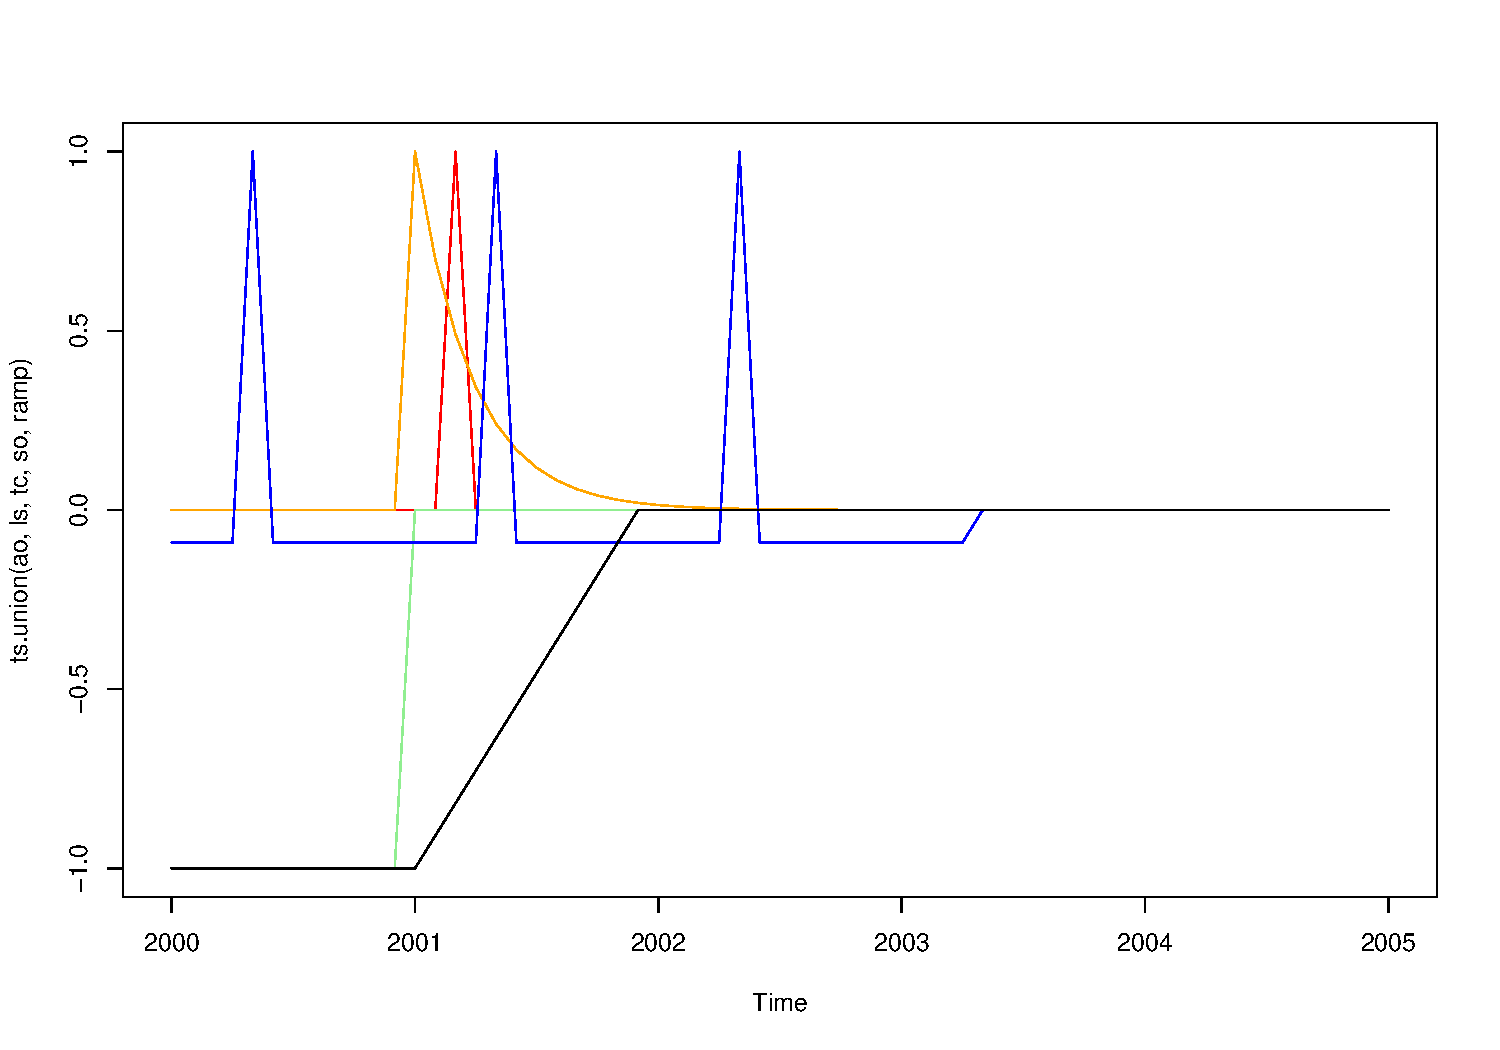
\includegraphics{img/markdown-outplot-1} \end{center}
\end{frame}

\hypertarget{time-series-tools}{%
\section{Time series tools}\label{time-series-tools}}

\begin{frame}[fragile]{Time series tools: NEW features in version 3}
\protect\hypertarget{time-series-tools-new-features-in-version-3}{}
The spirit of version 3 is to offer more tools from JDemetra+ libraries
such as:

\begin{itemize}
\item
  tests (seasonality, normality, randomness, residual td effects)
  (rjd3tookit, rjd3modelling; rjd3sa)
\item
  autocorrelation functions (irjd3toolkit), incl partial and inverse
\item
  arima model estimation and decomposition (rjd3modelling)
\item
  aggregation to higher frequency (\texttt{rjd3toolkit::aggregate()})
\end{itemize}

More flexibilty for the user as they can be applied any time not just as
part of an SA porcessing.

Some of might also be available in other R packages. Arima model
estimation is notoriously faster than other R functions.
\end{frame}

\begin{frame}[fragile]{Testing for seasonality}
\protect\hypertarget{testing-for-seasonality}{}
In rjd3sa:

\begin{itemize}
\item
  Canova-Hansen (\texttt{seasonality.canovahansen()})
\item
  X-12 combined test (\texttt{seasonality.combined()})
\item
  F-test on seasonal dummies (\texttt{seasonality.f()})
\item
  Friedman Seasonality Test (\texttt{seasonality.friedman()})
\item
  Kruskall-Wallis Seasonality Test
  (\texttt{seasonality.kruskalwallis()})
\item
  Periodogram Seasonality Test (\texttt{seasonality.periodogram()})
\item
  QS Seasonality Test (\texttt{seasonality.qs()})
\end{itemize}
\end{frame}

\begin{frame}[fragile,allowframebreaks]{Testing for seasonality:
examples}
\protect\hypertarget{testing-for-seasonality-examples}{}
(Always correct the trend and remove the mean before seasonality tests)

\footnotesize

\begin{Shaded}
\begin{Highlighting}[]
\FunctionTok{library}\NormalTok{(rjd3sa)}
\NormalTok{y }\OtherTok{=} \FunctionTok{diff}\NormalTok{(rjd3toolkit}\SpecialCharTok{::}\NormalTok{ABS}\SpecialCharTok{$}\NormalTok{X0.}\DecValTok{2}\NormalTok{.}\DecValTok{09}\NormalTok{.}\FloatTok{10.}\NormalTok{M, }\DecValTok{1}\NormalTok{); y }\OtherTok{=}\NormalTok{ y }\SpecialCharTok{{-}} \FunctionTok{mean}\NormalTok{(y)}
\FunctionTok{seasonality.f}\NormalTok{(y, }\DecValTok{12}\NormalTok{)}
\end{Highlighting}
\end{Shaded}

\begin{verbatim}
## Value:  378.9234 
## P-Value:  0.0000
\end{verbatim}

\begin{Shaded}
\begin{Highlighting}[]
\FunctionTok{seasonality.friedman}\NormalTok{(y, }\DecValTok{12}\NormalTok{)}
\end{Highlighting}
\end{Shaded}

\begin{verbatim}
## Value:  298.2529 
## P-Value:  0.0000
\end{verbatim}

\begin{Shaded}
\begin{Highlighting}[]
\FunctionTok{seasonality.kruskalwallis}\NormalTok{(y, }\DecValTok{12}\NormalTok{)}
\end{Highlighting}
\end{Shaded}

\begin{verbatim}
## Value:  319.9801 
## P-Value:  0.0000
\end{verbatim}

\begin{Shaded}
\begin{Highlighting}[]
\FunctionTok{seasonality.combined}\NormalTok{(y, }\DecValTok{12}\NormalTok{)}
\end{Highlighting}
\end{Shaded}

\begin{verbatim}
## $seasonality
## [1] "PRESENT"
## 
## $kruskalwallis
## $kruskalwallis$value
## [1] 319.9801
## 
## $kruskalwallis$pvalue
## [1] 0
## 
## $kruskalwallis$description
## [1] "Chi2 with 11.0 degrees of freedom "
## 
## 
## $stable
## $stable$SSM
## [1] 69596527
## 
## $stable$dfM
## [1] 11
## 
## $stable$SSR
## [1] 6721009
## 
## $stable$dfR
## [1] 412
## 
## $stable$test
## Value:  387.8445 
## P-Value:  0.0000 
## 
## 
## $evolutive
## $evolutive$SSM
## [1] 2145849
## 
## $evolutive$dfM
## [1] 34
## 
## $evolutive$SSR
## [1] 3800578
## 
## $evolutive$dfR
## [1] 374
## 
## $evolutive$test
## Value:  6.210723 
## P-Value:  0.0000
\end{verbatim}
\end{frame}

\begin{frame}[fragile]{Arima estimation}
\protect\hypertarget{arima-estimation}{}
\begin{Shaded}
\begin{Highlighting}[]
\CommentTok{\# JD+}
\FunctionTok{print}\NormalTok{(}\FunctionTok{system.time}\NormalTok{(}\ControlFlowTok{for}\NormalTok{ (i }\ControlFlowTok{in} \DecValTok{1}\SpecialCharTok{:}\DecValTok{1000}\NormalTok{) \{  j}\OtherTok{\textless{}{-}}\NormalTok{rjd3modelling}\SpecialCharTok{::}\FunctionTok{sarima.estimate}\NormalTok{(}\FunctionTok{log}\NormalTok{(rjd3toolkit}\SpecialCharTok{::}\NormalTok{ABS}\SpecialCharTok{$}\NormalTok{X0.}\DecValTok{2}\NormalTok{.}\DecValTok{09}\NormalTok{.}\FloatTok{10.}\NormalTok{M), }\AttributeTok{order=}\FunctionTok{c}\NormalTok{(}\DecValTok{2}\NormalTok{,}\DecValTok{1}\NormalTok{,}\DecValTok{1}\NormalTok{), }\AttributeTok{seasonal =} \FunctionTok{list}\NormalTok{(}\AttributeTok{order=}\FunctionTok{c}\NormalTok{(}\DecValTok{0}\NormalTok{,}\DecValTok{1}\NormalTok{,}\DecValTok{1}\NormalTok{), }\AttributeTok{period=}\DecValTok{12}\NormalTok{))\}))}

\CommentTok{\#utilisateur     système      écoulé }
\CommentTok{\#      4.98        0.37        4.63 }

\CommentTok{\#R{-}native}
\FunctionTok{print}\NormalTok{(}\FunctionTok{system.time}\NormalTok{(}\ControlFlowTok{for}\NormalTok{ (i }\ControlFlowTok{in} \DecValTok{1}\SpecialCharTok{:}\DecValTok{1000}\NormalTok{) \{  r}\OtherTok{\textless{}{-}}\FunctionTok{arima}\NormalTok{(}\FunctionTok{log}\NormalTok{(rjd3toolkit}\SpecialCharTok{::}\NormalTok{ABS}\SpecialCharTok{$}\NormalTok{X0.}\DecValTok{2}\NormalTok{.}\DecValTok{09}\NormalTok{.}\FloatTok{10.}\NormalTok{M), }\AttributeTok{order=}\FunctionTok{c}\NormalTok{(}\DecValTok{2}\NormalTok{,}\DecValTok{1}\NormalTok{,}\DecValTok{1}\NormalTok{), }\AttributeTok{seasonal =} \FunctionTok{list}\NormalTok{(}\AttributeTok{order=}\FunctionTok{c}\NormalTok{(}\DecValTok{0}\NormalTok{,}\DecValTok{1}\NormalTok{,}\DecValTok{1}\NormalTok{), }\AttributeTok{period=}\DecValTok{12}\NormalTok{))\}))}
\FunctionTok{print}\NormalTok{(j}\SpecialCharTok{$}\NormalTok{likelihood )}
\FunctionTok{print}\NormalTok{(r)}

\CommentTok{\# utilisateur     système      écoulé }
\CommentTok{\#     158.74        0.23      160.49 }
\end{Highlighting}
\end{Shaded}
\end{frame}

\hypertarget{conclusion}{%
\section{Conclusion}\label{conclusion}}

\begin{frame}{Conclusion on SA in R}
\protect\hypertarget{conclusion-on-sa-in-r}{}
What has v3 brought to the table ?
\end{frame}

\end{document}
